% Adding a coloured vertical edge to the pages in the chapter
\ClearShipoutPicture
\AddToShipoutPicture{%
  \AtPageLowerLeft{%
    \checkoddpage
    \ifoddpage
      \begin{tikzpicture}[remember picture,overlay] % Odd page → right edge
        \draw[line width=80pt, colour_chapter5] 
             (\paperwidth,0) -- (\paperwidth,\paperheight);
      \end{tikzpicture}%
    \else
      \begin{tikzpicture}[remember picture,overlay] % Even page → left edge
        \draw[line width=80pt, colour_chapter5] 
             (0,0) -- (0,\paperheight);
      \end{tikzpicture}%
    \fi
  }%
}

%%%%%%%%%%%%%%%%%%%%%%%%%%%%%%%%%%%%%%%%%%%%%%%%%%%%%%%%%%%
\chapter{Flash-flood-focused verification of rainfall-based 
predictions of areas at risk of flash floods}
\label{flash_flood_focused_verification_rainfall_based_ff}
\graphicspath{{chapter_05/figures}{chapter_05/tables}}
%%%%%%%%%%%%%%%%%%%%%%%%%%%%%%%%%%%%%%%%%%%%%%%%%%%%%%%%%%%

\underline{\textbf{Authors' contribution for this chapter:}} Fatima M. Pillosu designed the study, with advice from Hannah Cloke and Christel Prudhomme, obtained the datasets, carried out the analysis, and led the writing of the manuscript. All authors assisted with writing the manuscript. Overall, 90\% of the writing was undertaken by Fatima M. Pillosu.

\vspace{\baselineskip}

\section*{PREFACE}
\addcontentsline{toc}{section}{PREFACE}

The first main analysis chapter (Chapter \ref{flash_flood_focused_verification_rainfall_based_ff}) undertakes the flash-flood-focused evaluation of short- and medium-range post-processed probabilistic point-scale rainfall forecasts. Such forecasts have been shown to predict better than the raw ERA5 flash-flood-triggering localised extreme rainfall events \citep{Pillosu_2025a}. While such an improvement in the prediction of localised extreme rainfall should enable the improved detection of areas at risk of flash floods, a flash-flood-focused assessment is fundamental to determining the extent to which enhanced rainfall prediction accuracy translates into meaningful improvements in flash flood hazard identification. In this chapter, \textcolor{colour_chapter5}{research question 1 (RQ1) "Can post-processed global NWP rainfall forecasts successfully identify areas at risk of flash floods up to medium-range lead times?"} is answered. Moreover, the first research component of this thesis is addressed, i.e. \textcolor{colour_chapter5}{developing a flash-flood-focused verification framework for predictions of areas at risk of flash floods, designed to benchmark the capability of different predictive systems}. Hence, this evaluation establishes a performance benchmark against which more sophisticated modelling approaches - incorporating additional hydrological and topographical parameters - can be measured. Such comparative analysis is essential for determining whether the increased computational demands and data requirements of complex systems yield commensurate improvements in flash flood prediction accuracy, or whether simpler precipitation-based approaches provide sufficient utility for early warning applications.

\clearpage

\section*{ABSTRACT}
\addcontentsline{toc}{section}{ABSTRACT}

\clearpage



%%%%%%%%%%%%%%%%%%%%%%
\section{Introduction}

Flash floods cause significant societal, economic, and environmental impacts \citep{Dordevic_2020}. These events arise through two primary mechanisms. The first involves intense, short-duration rainfall events (typically less than 6 hours) that generate rapid surface runoff and channel response, particularly over steep slopes. The second occurs when sustained moderate-to-extreme rainfall over extended periods (> 6 hours) progressively saturates soils, reducing infiltration rates and promoting surface runoff that inundates low-lying areas \citep{Speight_2021}. Short-duration flash flood events typically result from small-scale convective systems, whilst prolonged events are more frequently associated with large-scale, mesoscale convective systems or hurricanes \citep{Doswell_2001}. The distinction between these mechanisms is essential as they exhibit different temporal scales, spatial patterns, and relationships with antecedent catchment conditions, and predictability limits. This study aims to enhance preparedness and mitigation strategies against this escalating threat, particularly in regions with limited resources and data, by assessing the effectiveness of global rainfall forecasts in identifying areas at risk of flash floods.

\begin{tcolorbox}[
  colframe=colour_chapter5, % Use the custom HEX colour for the vertical line
  colback=white,            % Background colour remains white
  sharp corners,            % Ensures sharp edges
  boxrule=2mm,              % Thickness of the left vertical line
  left=0mm,                 % Space inside the left margin
  right=0mm,                % No space on the right
  toprule=0mm,              % Remove the top border
  bottomrule=0mm,           % Remove the bottom border
  rightrule=2mm            % Remove the right border
]
{\color{colour_chapter5} {\setlength{\parindent}{1.0em} The term \textbf{"identification of areas at risk of flash floods"} refers to the \textit{prediction of polygons - or areas - that might experience flash flooding due to the expected rainfall}.}}
\end{tcolorbox}

Forecast-triggered mitigation strategies, such as early warning systems \citep{CoughlanDePerez_2022, ŠakićTrogrlić_2022} and forecast-based financing protocols \citep{Bischiniotis_2019a, Perez_2016}, have been shown to improve resilience, decrease mortality, and lower recovery costs against riverine floods. Yet, these strategies hinge on accurate, timely predictions. In lower-income countries, accurate forecasts with even longer lead times are required to set cost-effective mitigation strategies \citep{Bazo_2019, Kiptum_2023}. 

Over the years, flash flood forecasting systems have been developed at local/regional \citep{Speight_2018, Corral_2019, Ibarreche_2020, RamosFilho_2021, Shuvo_2021}, national \citep{Javelle_2016, Liu_2018}, and continental scales \citep{Gourley_2017, Raynaud_2015}, with varying degrees of model complexity and forecast accuracy. These systems share a reliance on high-density rainfall and discharge observations, and km-scale rainfall forecasts \citep{Braud_2014}. This approach has prevented the development of a flash flood forecasting system that provides medium-range forecasts over a continuous global domain. Radar-derived rainfall predictions remain limited to a few hours ahead \citep{Imhoff_2022}, and kilometre-scale forecasts show substantial skill reduction beyond two days \citep{Barrett_2019}. Moreover, the uneven spatial distribution of these data sources restricts flash flood prediction to a collection of separate regional and national systems, including WMO's "Flash Flood Guidance System with Global Coverage" \citep{Georgakakos_2022}. Consequently, many areas of the world remain without access to flash flood guidance, highlighting the need for alternative approaches to address the challenge of providing medium-range predictions of areas at risk of flash floods over a continuous global domain.

Global NWP models, such as ECMWF’s IFS, are increasingly seen as a viable solution to this challenge. These models provide daily global rainfall predictions up to medium-range leads but have historically struggled to accurately predict extreme localised rainfall events due to their coarse resolution and parametrisation schemes \citep{Emerton_2016, Wen_2021}. Owing to recent improvements in global NWP forecast accuracy \citep{Haiden_2023, Lavers_2021}, the interest in using them to provide flash flood guidance in data-scarce regions and extend predictions’ lead times has recently increased \citep{Bucherie_2022b}. Additionally, the development of state-of-the-art post-processing techniques can enhance the quality of raw forecasts and make them more suitable for flash flood prediction \citep{Vannitsem_2021}. For example, the ecPoint statistical post-processing technique transforms global grid-based forecasts into probabilistic point-scale predictions, improving the reliability and discrimination ability of rainfall forecasts up to day 10, especially for extremes \citep{Hewson_2021}.

Since a significant gap remains in leveraging global rainfall NWP forecasts for flash flood forecasting, this study aims to bridge this gap by evaluating the performance of ERA5-ecPoint rainfall forecasts in identifying areas at risk of flash floods. The CONUS, with its extensive collection of flash flood impact reports within NOAA's Storm Event Database and its varying climate, serves as an ideal test bed for this research. The research question posed in this study is \textit{can post-processed global NWP rainfall forecasts successfully identify areas at risk of flash floods up to medium-range lead times?} The innovation proposed by this research is twofold. It first proposes a flash-flood-focused verification framework for predictions of areas at risk of flash floods, in recognition of the non-linear relationship between flash floods and triggering rainfall events. Hence, this framework can be used as a common framework to benchmark the general capabilities of different systems to predict areas at risk of flash floods. This research also provides a performance benchmark against which more sophisticated modelling approaches - incorporating additional hydrological and topographical parameters - can be measured. Such comparative analysis is essential for determining whether the increased computational demands and data requirements of complex systems yield commensurate improvements in flash flood prediction accuracy, or whether simpler precipitation-based approaches provide sufficient utility for early warning applications.

% TO BE INCORPORATED IN THE INTRODUCTION: The application of the flash-flood-focused verification framework to the identification of areas at risk of flash floods involving solely rainfall predictions is done in the recognition that a robust understanding of rainfall forecast performance in identifying areas at risk of flash floods is essential to benchmark the performance of more advanced prediction methods, e.g. data-driven approaches involving more parameters.

This chapter is organised as follows. Sections \ref{flash_flood_focused_verification_rainfall_based_ff_DATA} and \ref{flash_flood_focused_verification_rainfall_based_ff_METHODS} describe the data and methods used to develop the flash-flood-focused verification framework. Section \ref{flash_flood_focused_verification_rainfall_based_ff_RESULTS} presents the results of the objective verification analysis, while section \ref{flash_flood_focused_verification_rainfall_based_ff_CASE_STUDY} presents results from a case-study-based subjective verification analysis. Section \ref{flash_flood_focused_verification_rainfall_based_ff_DISCUSSIONS} discusses the verification results, while section \ref{flash_flood_focused_verification_rainfall_based_ff_CONCLUSIONS} draws concluding remarks for the study.


%%%%%%%%%%%%%%
\section{Data}
\label{flash_flood_focused_verification_rainfall_based_ff_DATA}


\subsection{Study domain}

This research establishes the CONUS as the primary study domain (see Figure \ref{fig:conus_domain}). The CONUS domain presents diverse hydro-meteorological conditions, encompassing varied topographical features ranging from coastal plains to mountainous terrain, and climatic regimes spanning Mediterranean, continental, subtropical, and desert classifications. This diversity encompasses a broad spectrum of flash-flood-generating mechanisms, ranging from intense convective precipitation to rain-on-snow events, thereby enhancing the potential for future transferability to global applications.

\begin{figure}[htbp]
\centering
\includegraphics[scale=0.65]{conus_domain_orography.png}
\caption{\textbf{CONUS domain.} The figure shows the orography at 1 km resolution (in shades of green and brown) and the location of the 25 most populated cities (black dots) over the CONUS.}
\label{fig:conus_domain}
\end{figure}

\subsection{Observations: NOAA's Storm Event Database}

The selection of the CONUS as the primary domain also lies on the high quality and comprehensiveness of NOAA's Storm Event Database. This database systematically records flash flood occurrences with high spatial and temporal resolution, including crucial metadata regarding impact severity, affected areas, and casualty information. The database's consistent reporting protocols and rigorous quality control procedures mitigate the observational uncertainty that typically plagues flash flood research \citep{Panwar_2020}.

The Storm Event Database serves as the US's official repository of severe weather records, including flash floods. Flash flood records began in 1996, with significant improvements in geographical precision implemented in 2007, when reporting transitioned from county-level to polygon-based representation, later extended to reports from 2001\footnote{\url{https://inside.nssl.noaa.gov/flash/database/}}.

The database covers the entire United States and territories with a spatial bounding box from 172.0°W to 65.0°E longitude and 18.0°N to 72.0°N latitude\footnote{\url{https://www.ncei.noaa.gov/access/metadata/landing-page/bin/iso?id=gov.noaa.ncdc:C00510}}. Data collection involves a network of 123 Natioanl Weather Service Forecast Offices gathering information from emergency management officials, law enforcement, trained SKYWARN spotters, damage surveys, media reports, and public observations\footnote{\url{https://www.ncdc.noaa.gov/stormevents/faq.jsp}}.

The Storm Event provides extensive metadata for flash flood events. Among all the available keys, we considered in this study only the keys described in Table 3. Although professional meteorologists and hydrologists collect flash flood reports to include in the Severe Storm Database, any human augmented reporting system is subject to variations in population density, diurnal cycles of human activity, and more mundane transcription or memory errors that affect the timing and location of reports \citep{Barthold_2015}. Evidence of these issues has been found in assessments of FFG skill \citep{Clark_2014}, and it has been found that the distribution of SED's flash flood reports is affected by the distribution of human population \cite{Marjerison_2016}. 

\begin{figure}[htbp]
\centering
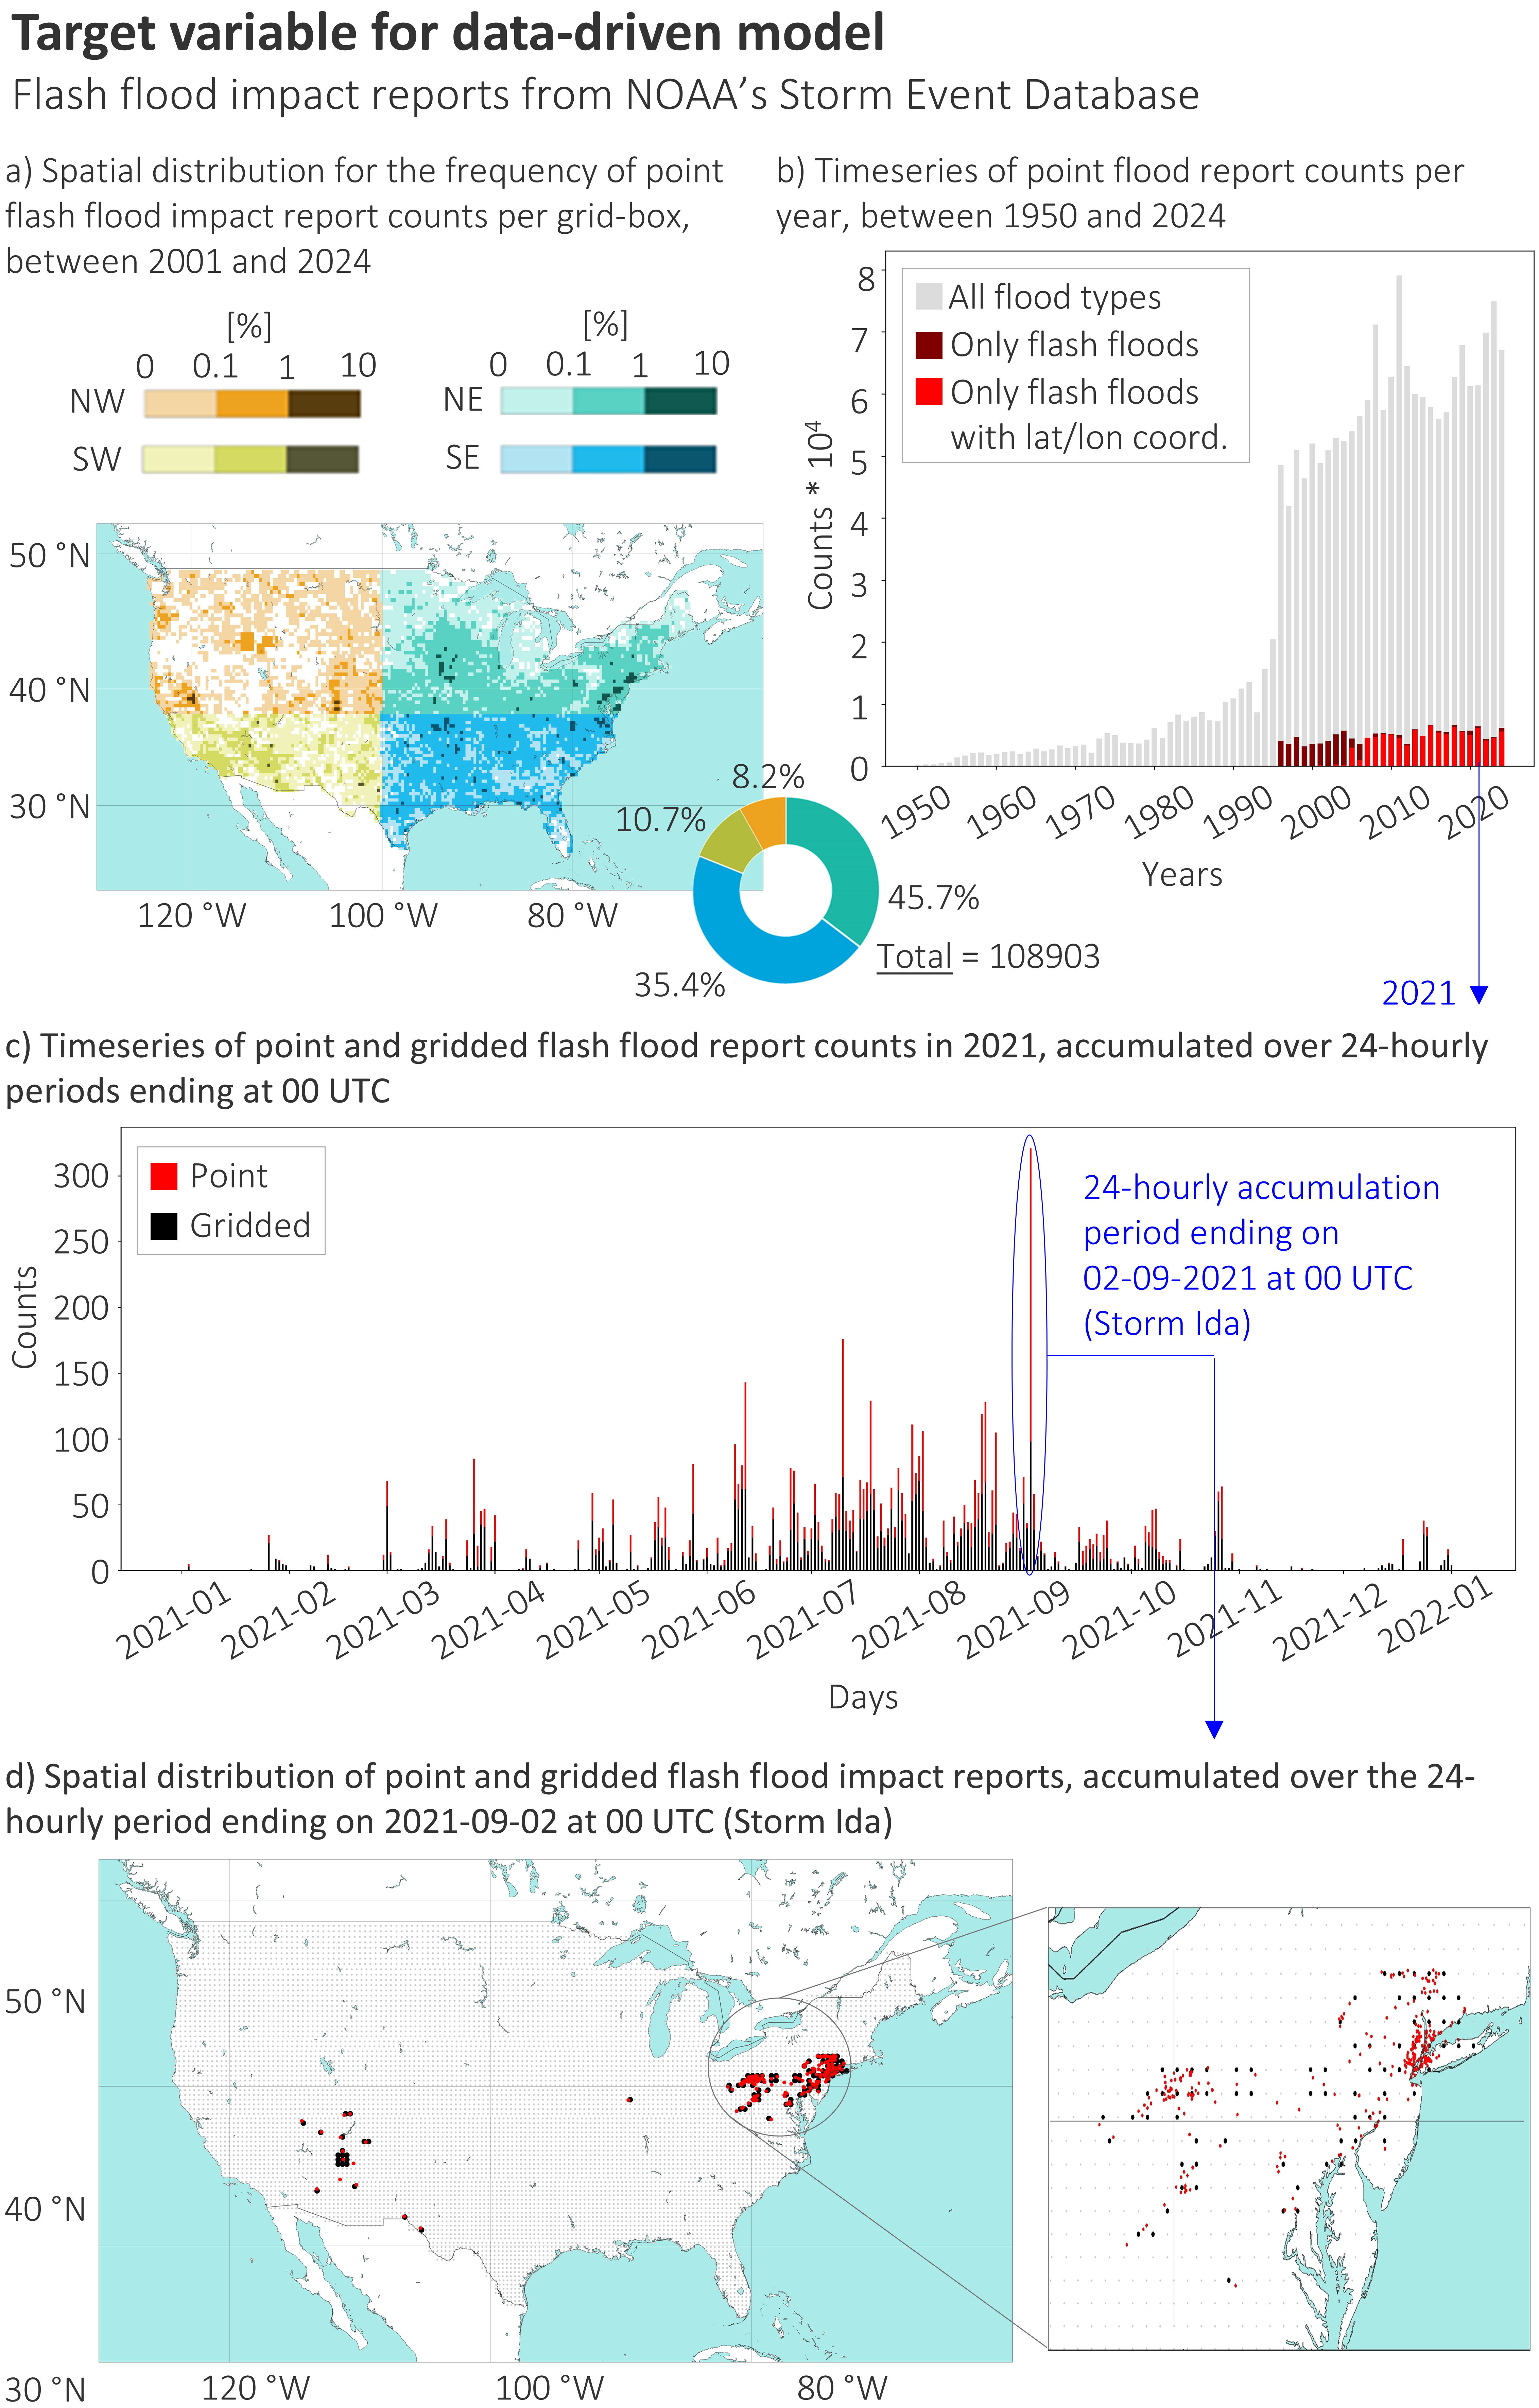
\includegraphics[scale = 0.85]{sed_ff_reports.png}
\caption{\textbf{Flash flood reports from NOAA's Storm Event Database.} Panel (a) displays the timeseries of flood reports from 1950 to 2024, distinguishing between all flood types (grey bars), only flash floods (dark red bars), and only flash flood reports with latitude/longitude coordinates (bright red bars) for the period 2001-2024. Panel (b) presents the spatial distribution of point flash flood report frequency per grid box for the period 2001-2024, shown as percentages (\%) across four geographical quadrants (North-West (NW, in shades of orange), South-West (SW, in shades of yellow), North-East (NE, in shades of green), South-East (SE, in shades of blue)) of the CONUS. The pie chart indicates the relative proportion of reports by region, with a total of 108,903 flash flood events reported in the considered period. Panel (c) illustrates the daily distribution of flash flood reports throughout 2021, showing both point reports (red bars) and gridded reports (black bars) accumulated over 24-hour periods ending at 00 UTC. The highlighted date with the blue circle (2nd September 2021) corresponds to the flash flood reports recorded during Storm Ida. Panel (d) maps the spatial distribution of flash flood reports, accumulated over the 24-hourly period ending at 00 UTC on 2 September 2021, displaying point reports with red dots and gridded reports with black dots. The zoomed-in box shows the reports recorded on the NE coast during Storm Ida.}
\label{fig:sed_ff_reports}
\end{figure}

In this study, we are using version 3.1 of the database, and we consider only reports over the CONUS that go from 2001 to 2024. 


\subsection{Rainfall forecasts: ERA5-ecPoint}

\begin{figure}[htbp]
\centering
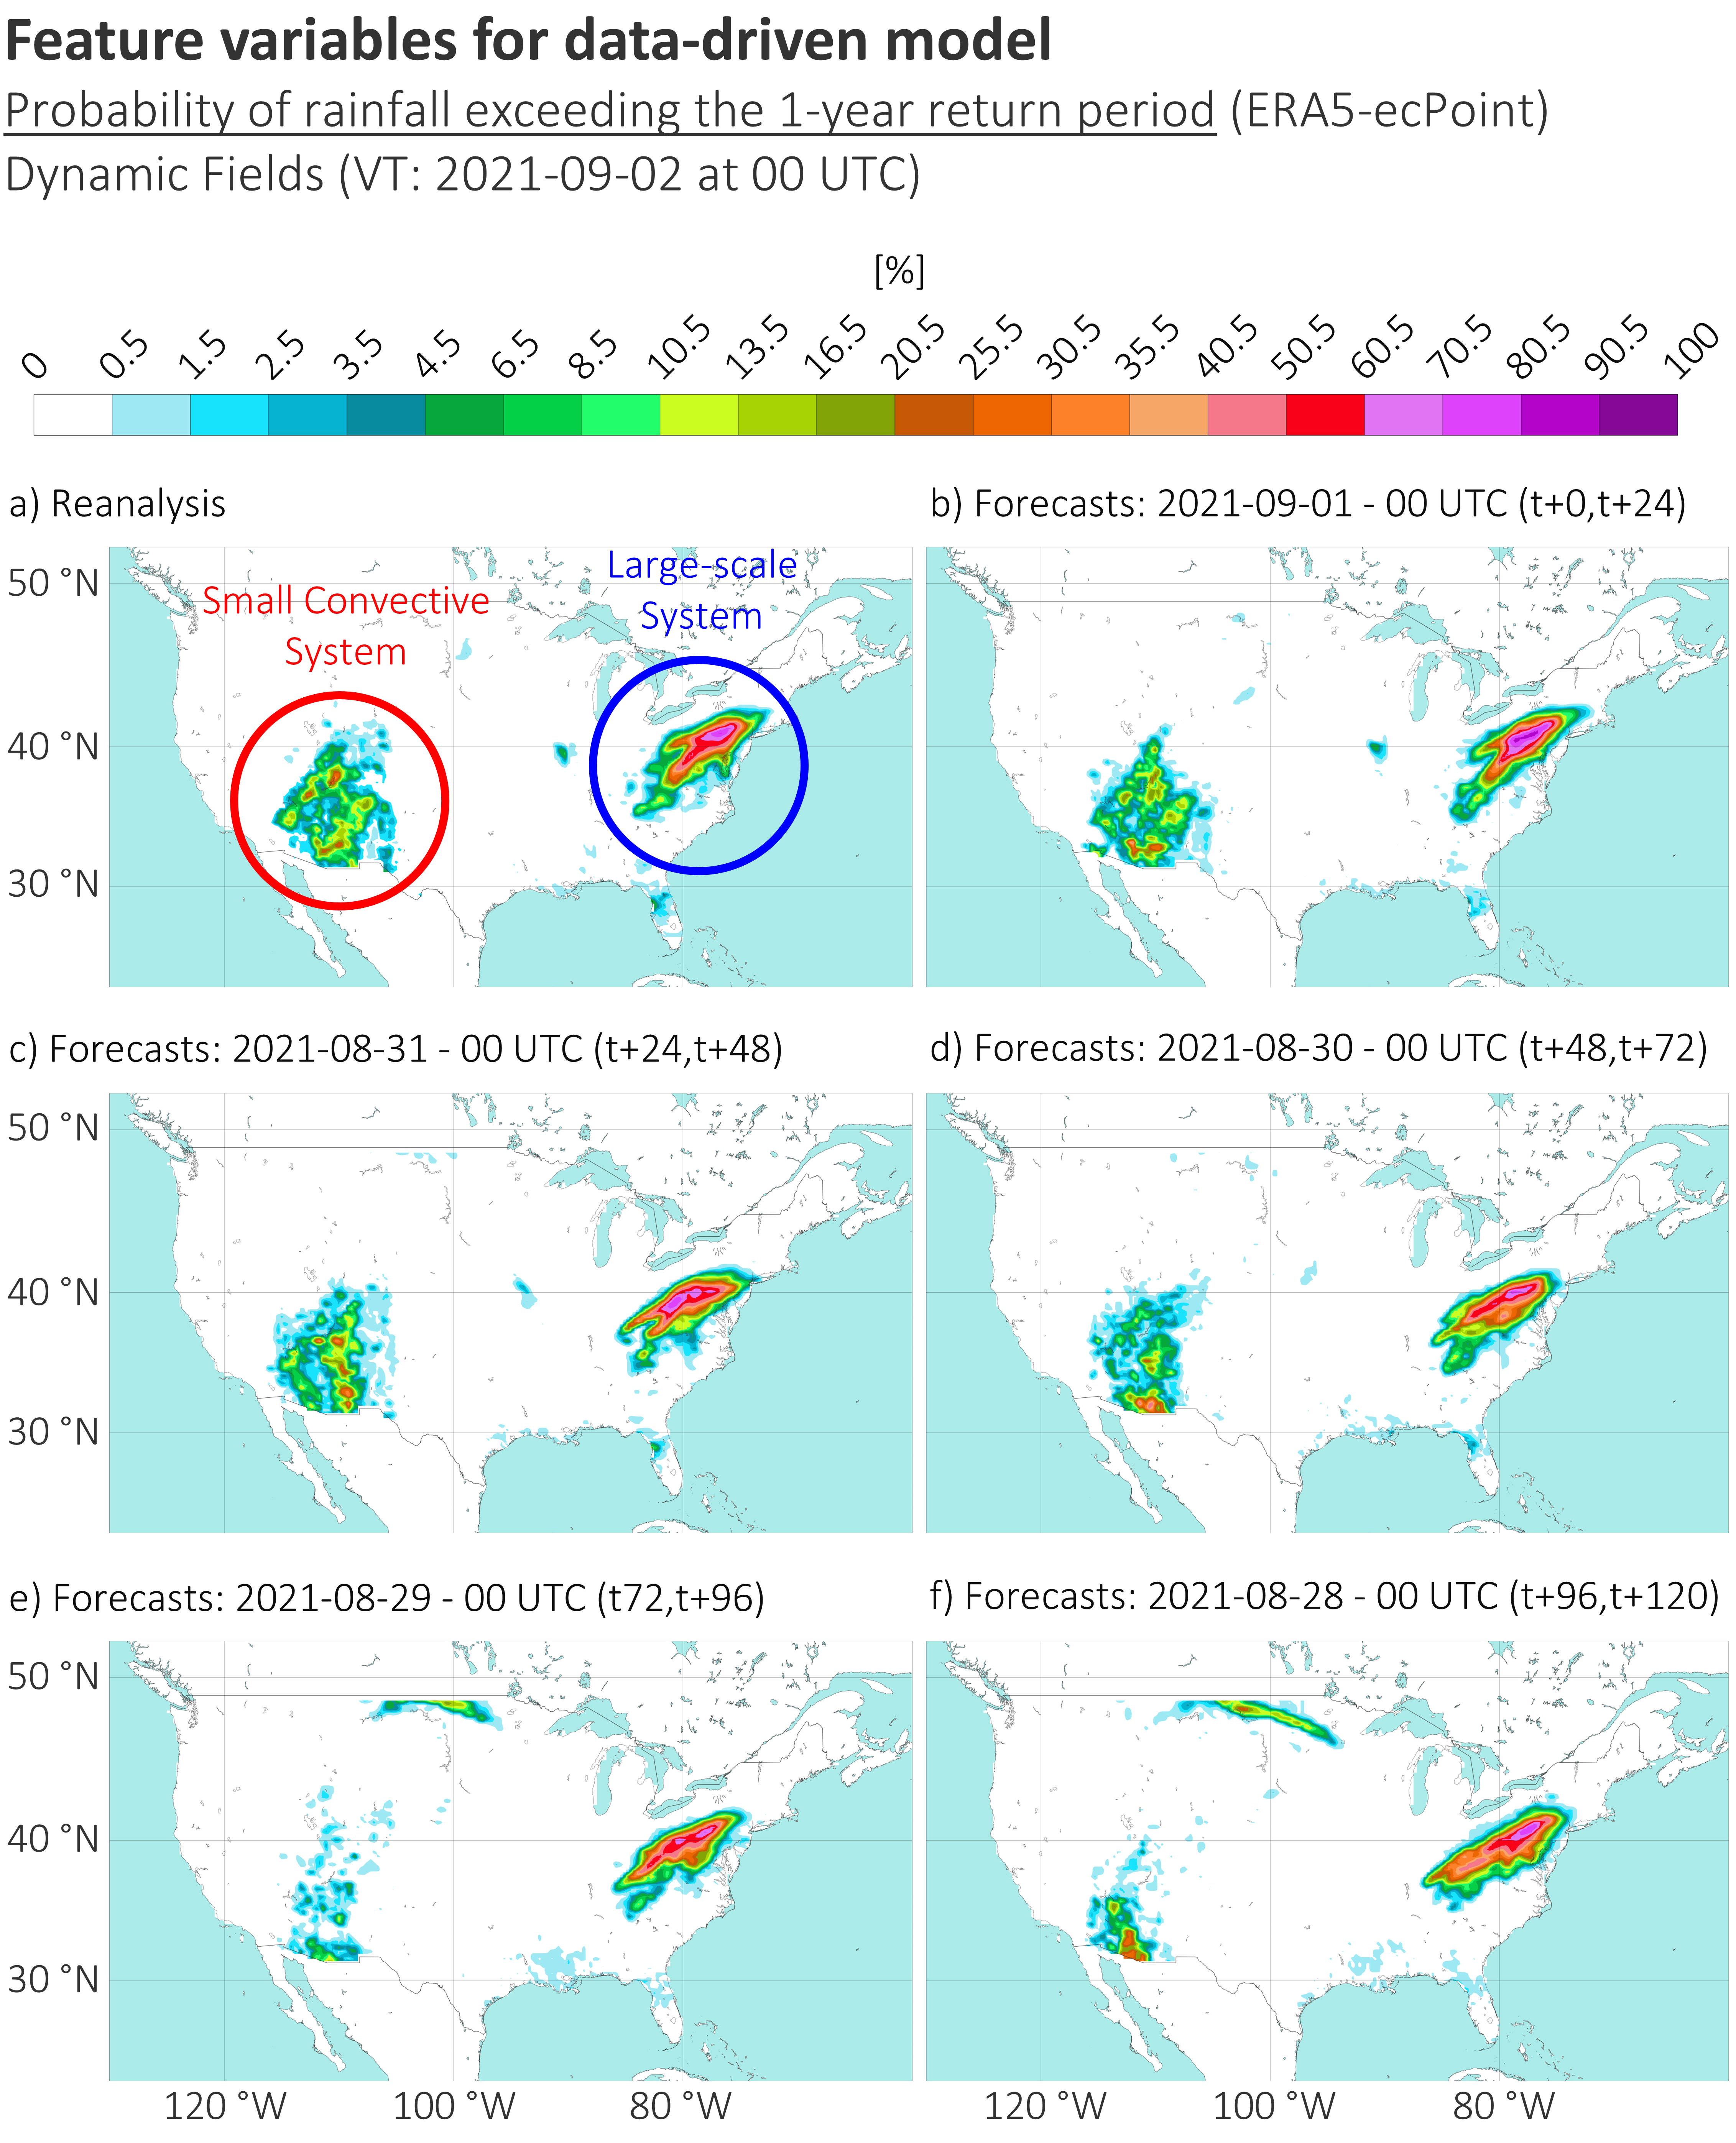
\includegraphics[width=\textwidth]{prob_tp_exceeding_1rp.png}
\caption{\textbf{Probability (\%) of exceeding the 1-year return period in ERA5-ecPoint.} Panel (a) displays probabilities in ERA5-ecPoint reanalysis for the valid time (VT) ending on 2021-09-02 at 00 UTC. Panels (b) to (f) represent the probabilities in ERA5-ecPoint forecasts for the same VT, but for forecasts at day 1 (t+0,t+24), day 2 (t+24,t+48), day 3 (t+48,t+72), day 4 (t+72,t+96), and day 5 (t+96,t+120), respectively.}
\label{fig:prob_tp_exceeding_1rp}
\end{figure}

ecPoint is a decision-tree-based statistical post-processing technique that transforms global grid-based forecasts into probabilistic point-scale forecasts \citep{Hewson_2021}. The post-processing technique aims to provide forecasts that mirror observations from rain gauges by addressing the two main factors affecting the performance of global NWP model outputs against point verification: systematic biases \citep{Lavers_2021} and lack of information on forecast sub-grid variability \citep{Göber_2008}. For each deterministic realisation or raw ensemble member of a probabilistic system, ecPoint generates an ensemble of X (e.g., 100) point-rainfall values based on the error distributions between forecasts and observations that vary according to different weather scenarios at the grid-box level. For example, when the model is on a grid-box, it primarily predicts large-scale rainfall with light winds. The raw model output tends to be representative of point rainfall totals within that grid-box, and ecPoint generates an ensemble with a smaller spread compared to the case of mainly convective rainfall with light winds. In the latter case, many points within the grid-box are expected to show zero rainfall, while large rainfall amounts may be observed at a few data points. The deterministic realisations of ERA5 reanalysis and forecasts were post-processed, creating a distribution of 100 point-rainfall totals, and distilled in 99 percentiles from 1st to 99th. ecPoint reanalysis and forecasts are provided in the same native grid of ERA5 (reduced Gaussian grid N320, \sim31 km), with forecasts up to day 5, and accumulation periods ending at 00 UTC.

\begin{figure}[htbp]
\centering
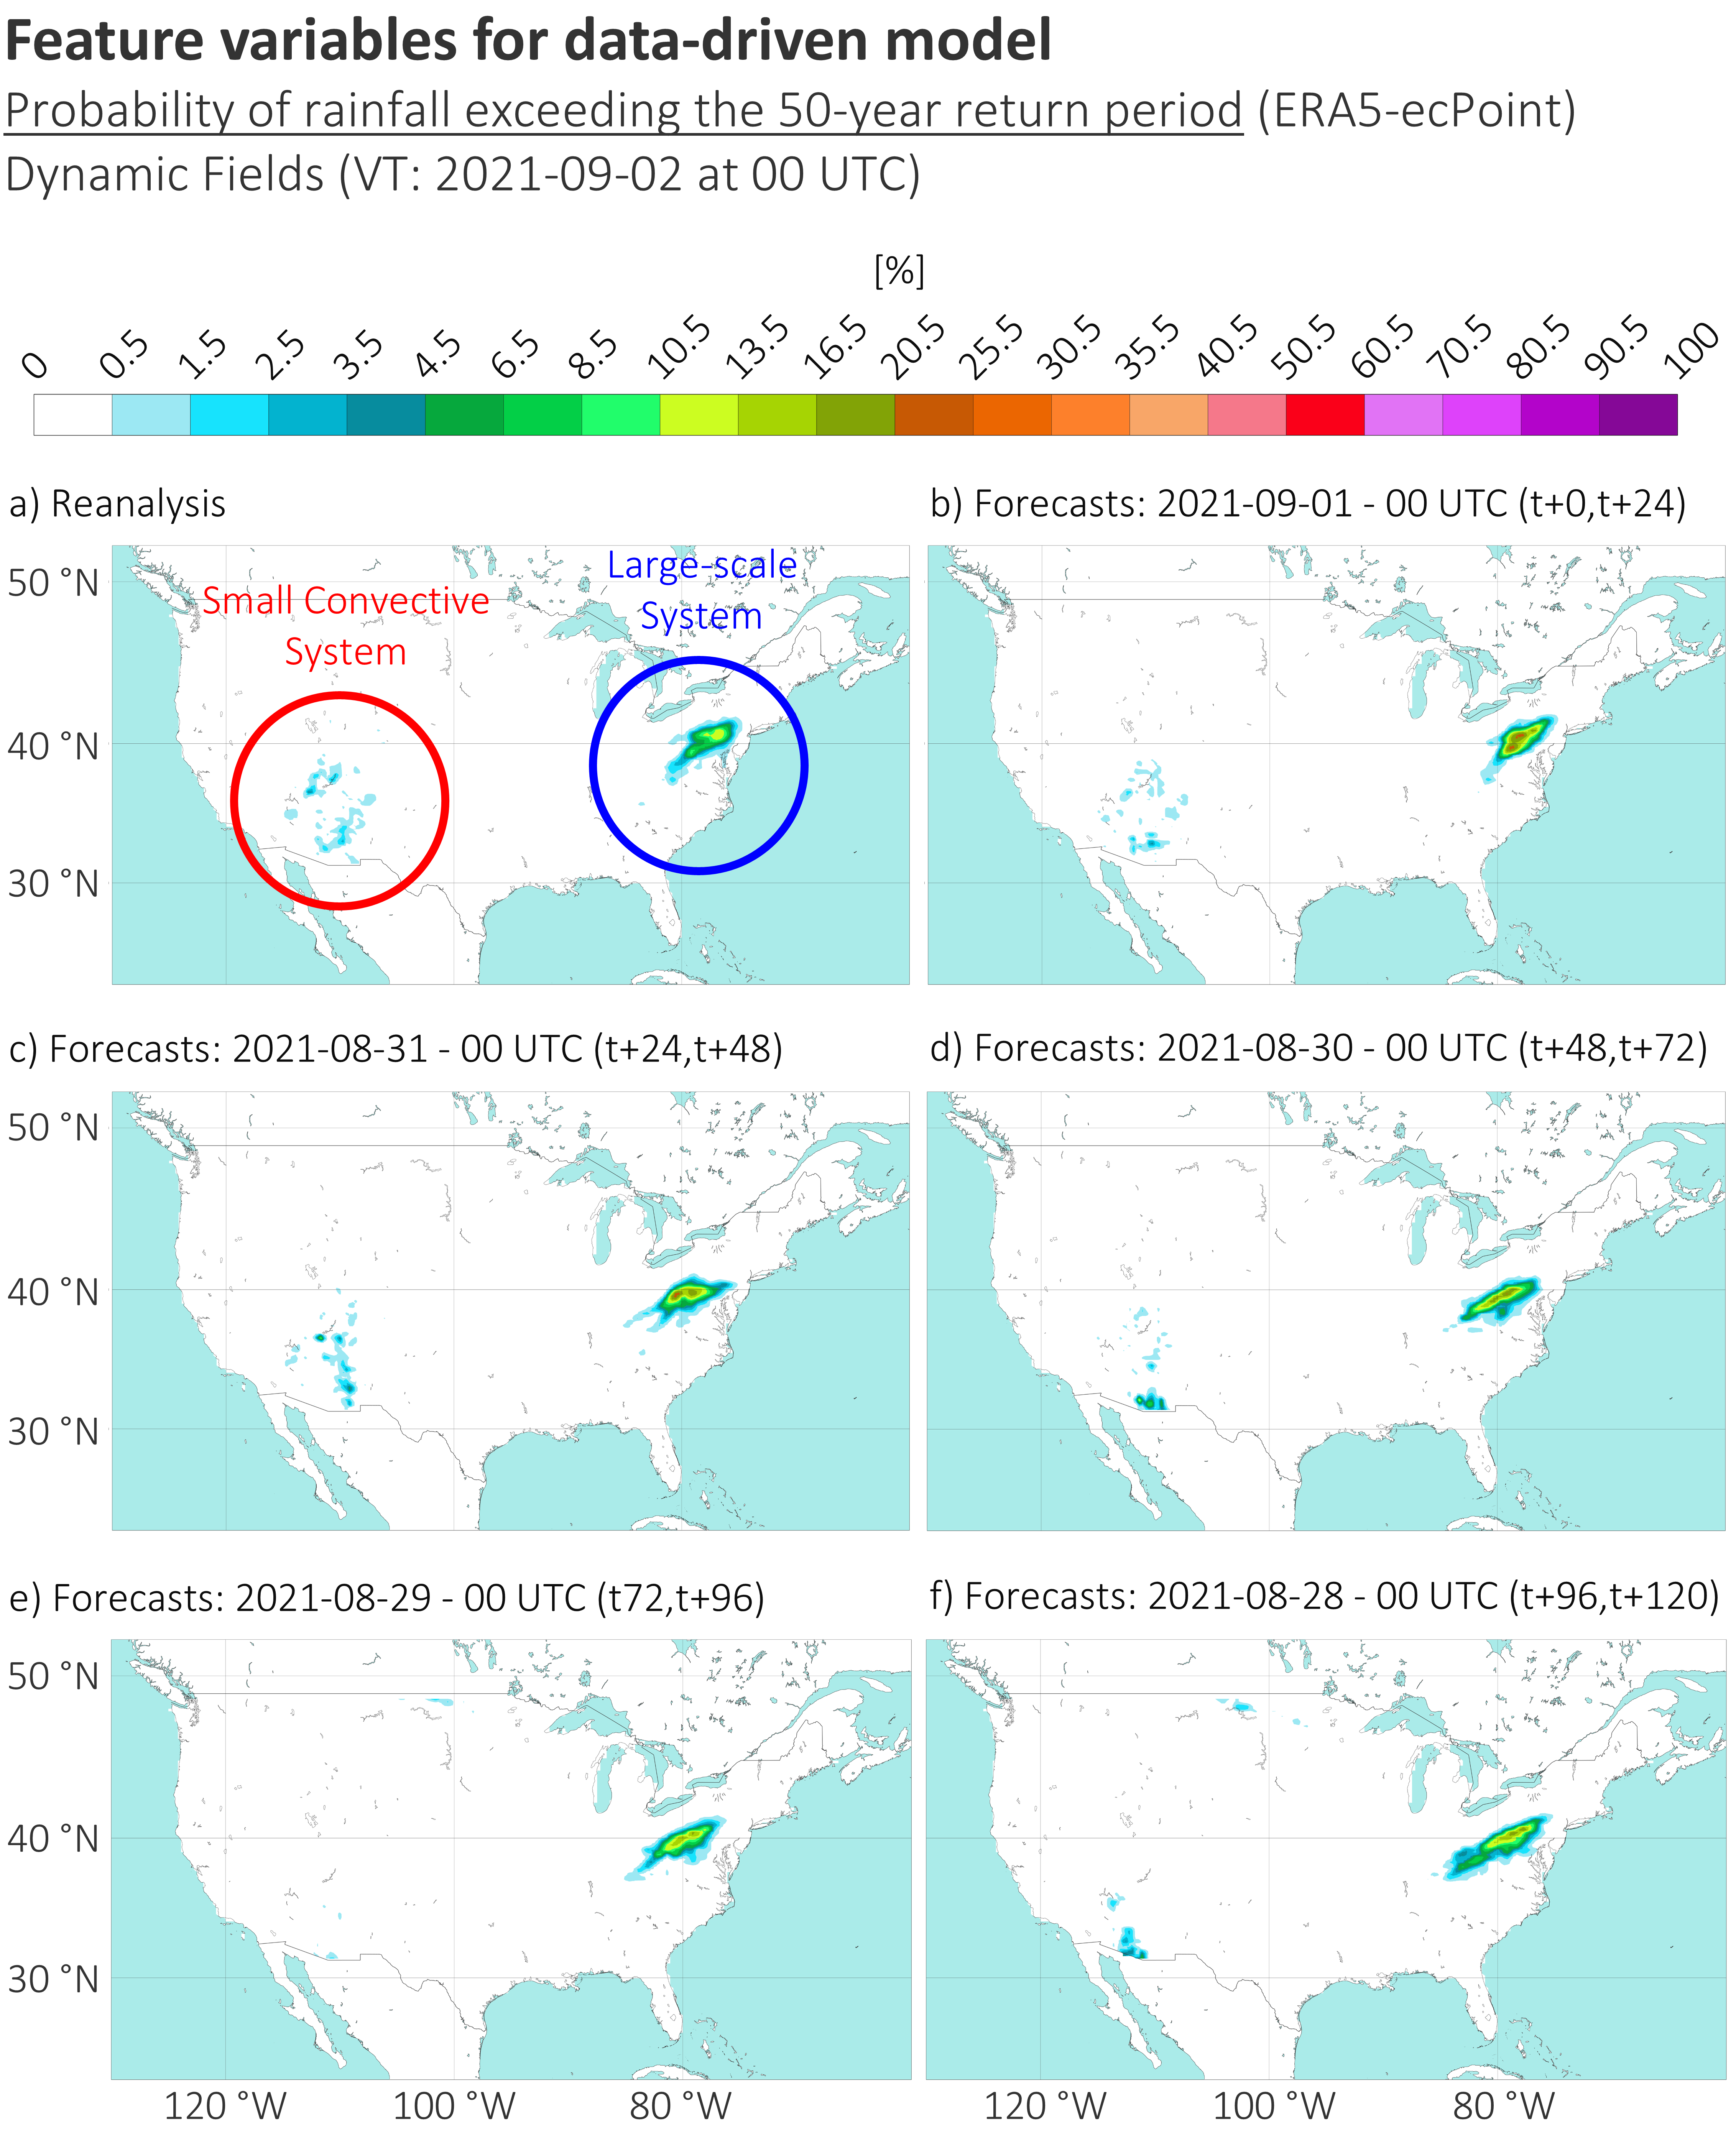
\includegraphics[width=\textwidth]{prob_tp_exceeding_50rp.png}
\caption{\textbf{Probability (\%) of exceeding the 50-year return period in ERA5-ecPoint.} Similar to Figure \ref{fig:prob_tp_exceeding_1rp}, but for probability of exceeding the 50-year return period.}
\label{fig:prob_tp_exceeding_50rp}
\end{figure}

Figure \ref{fig:prob_tp_exceeding_1rp} and \ref{fig:prob_tp_exceeding_50rp} show examples of the probabilities of exceeding the 1-year and 50-year return period in ERA5-ecPoint reanalysis and forecasts. It is worth noting that the ecPoint technique does not increase or decrease the probabilities of exceeding a certain threshold everywhere in the same way. In the example shown, the NE coast of the CONUS was affected by Storm Ida (a large-scale convective system). In this case, the probabilities of exceeding the 1-year and the 50-year return periods are uniformly large over a large area, indicating that this event might be fairly widespread. The signal remains fairly strong (with probabilities > 60\%) up to day 5 forecasts, showing a good predictability for this particular system. Over the SW quadrant of the CONUS, we can notice a large "bubbly" area of fairly large (> 20\%). The "bubbly" shape indicates the likelihood of very localised intense rainfall events from a small-scale convective system. The predictability of the event varies with increasing lead times, with the area being affected by intense rainfall decreasing for longer lead times, as well as the probabilities of experiencing intense rainfall. In this case, predicting the correct areas that may experience intense rainfall is more difficult as the predictions vary significantly over time.


%%%%%%%%%%%%%%%%%
\section{Methods: development of an objective flash-flood-focused verification framework for predictions of areas at risk of flash floods}
\label{flash_flood_focused_verification_rainfall_based_ff_METHODS}

\begin{figure}[htbp]
\centering
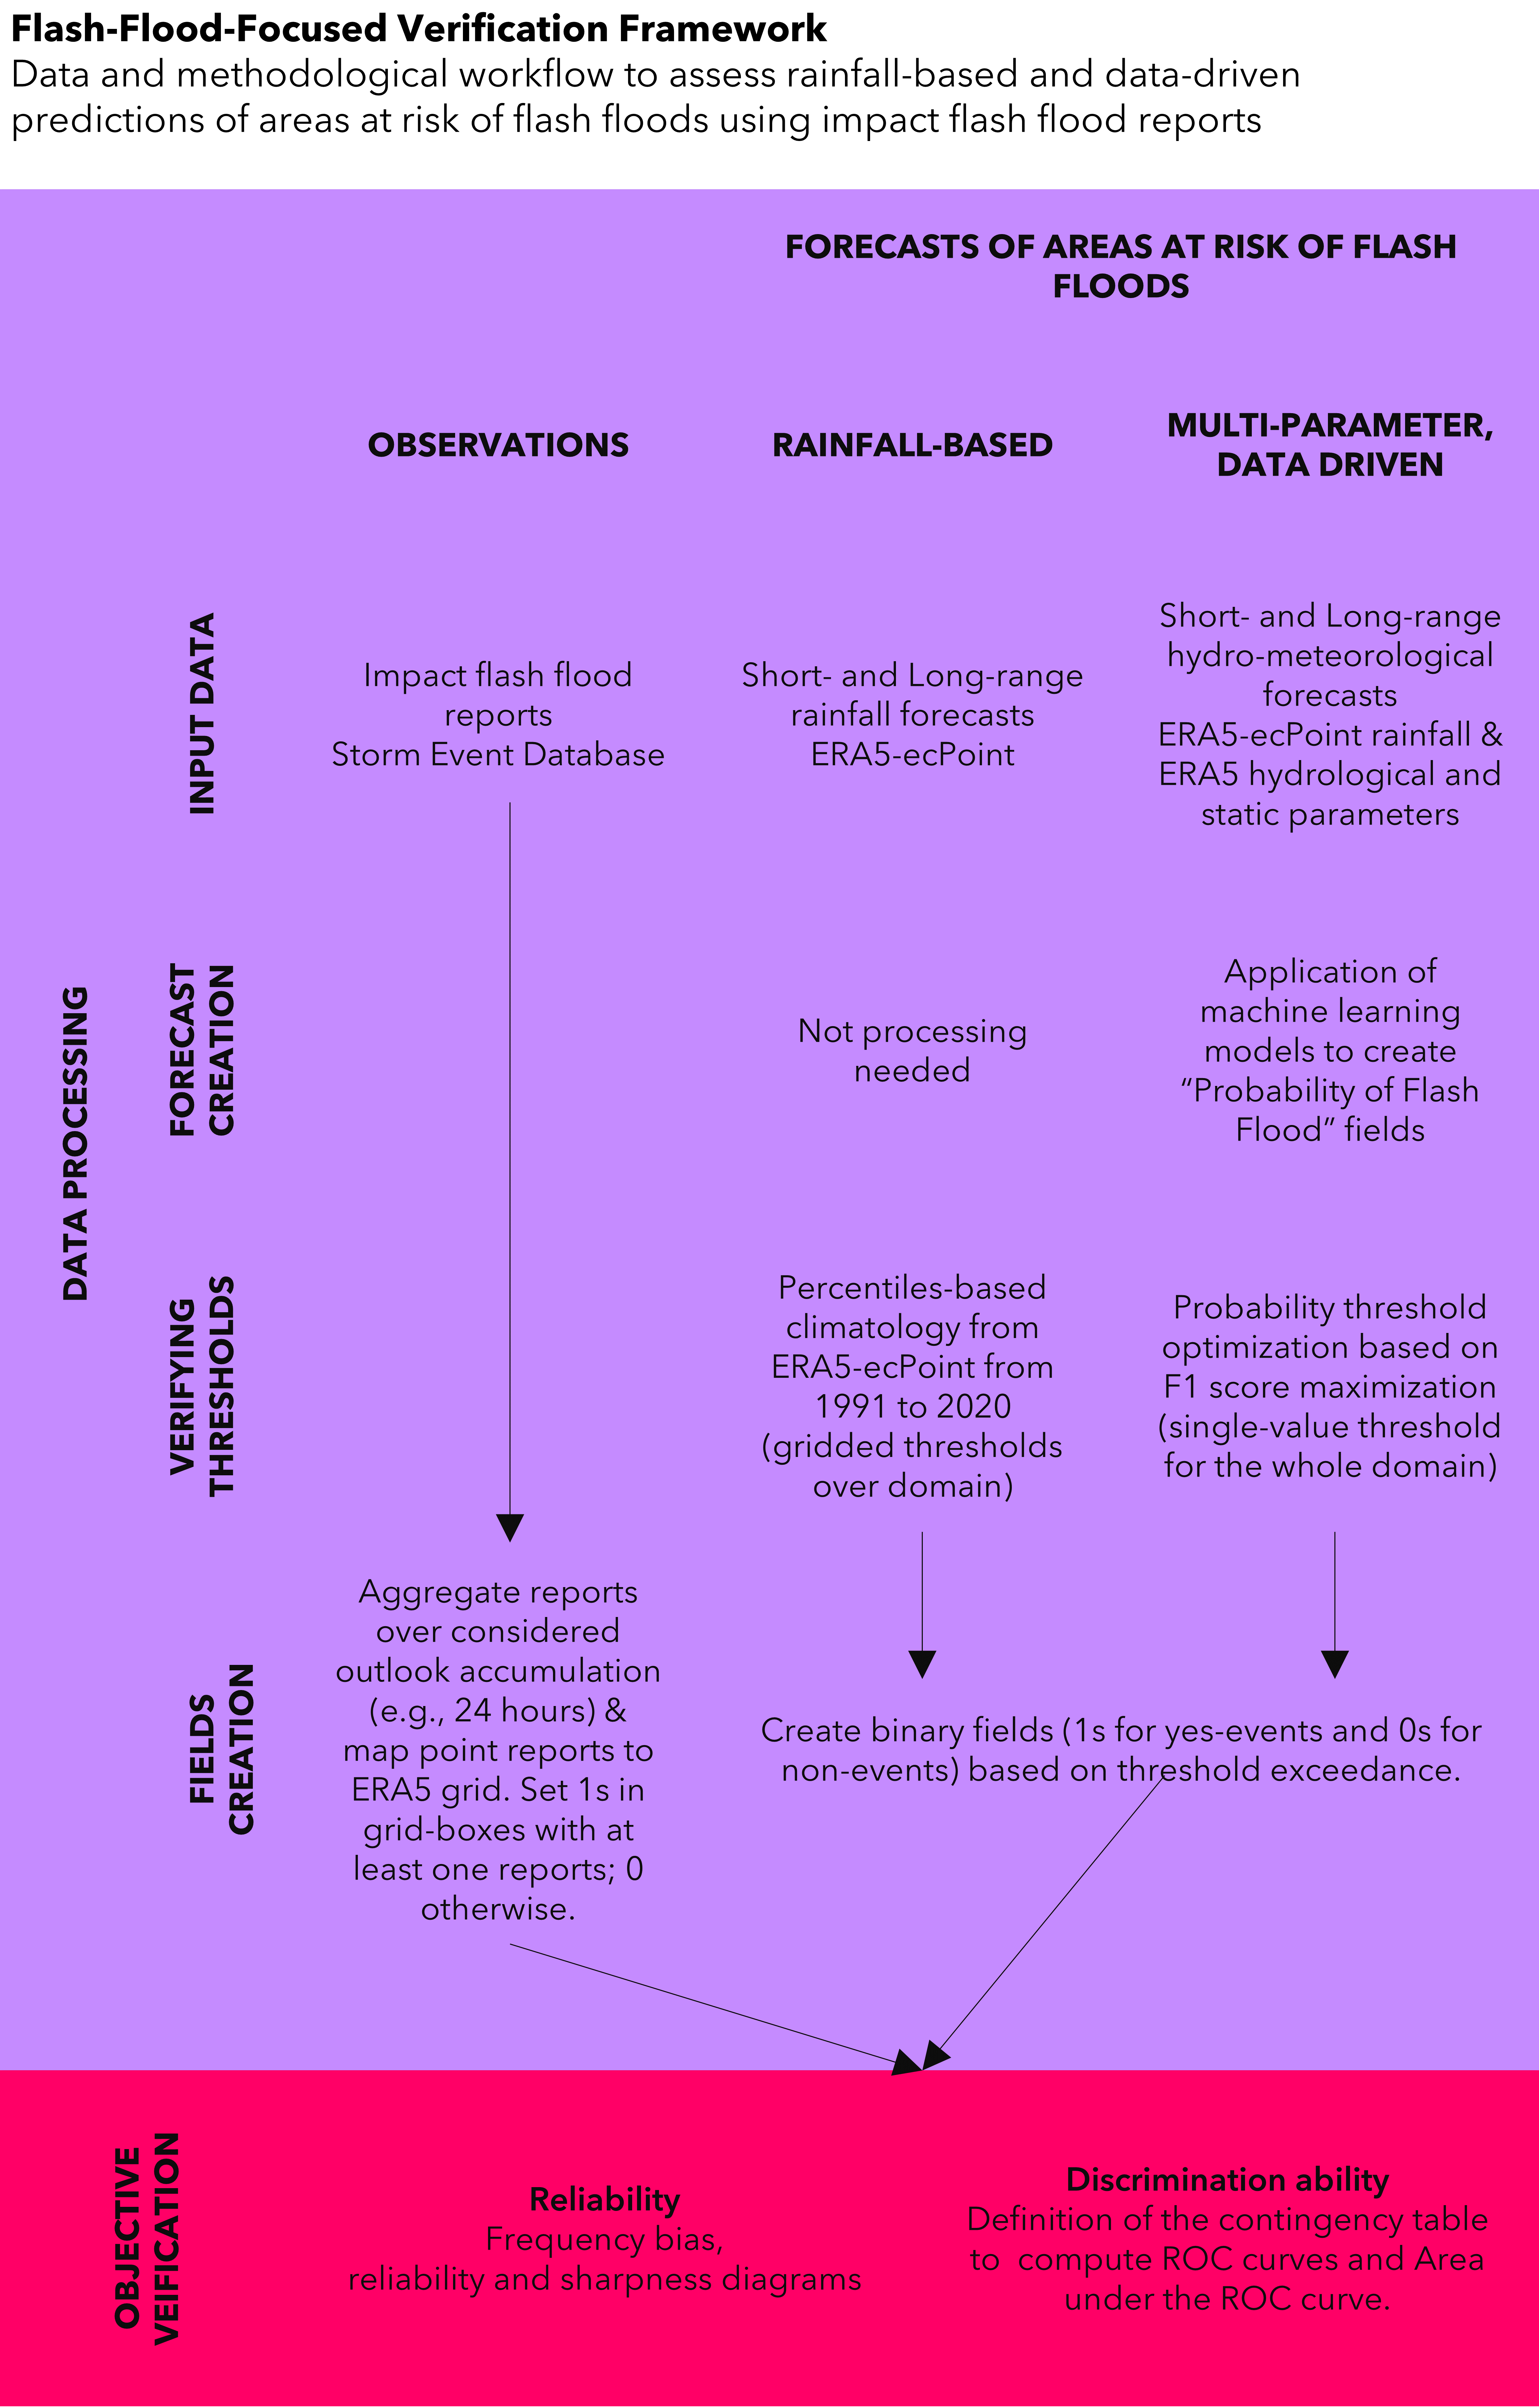
\includegraphics[width=\textwidth]{workflow_verif_framework.png}
\caption{\textbf{Workflow for flash-flood-focused verification framework.}}
\label{fig:sed_reports}
\end{figure}

\subsection{Observational fields}
The objective verification framework proposed in this thesis uses flash flood impact reports as ground truth. As indicated in section \ref{storm_event_database}, this thesis will consider only the Storm Event Database over the CONUS. However, this method can be applied in other geographical regions where regional databases are available, such as over Europe (using the ESWD dataset) or a global domain (considering global datasets such as EM-DAT), while always acknowledging the biases that such impact databases might possess. 

The definition of the observational dataset follows the methodology proposed by \citep{Tsonevsky_2018} for severe weather, and \citep{Pillosu_2024} for flash floods in Ecuador. Each flash flood report was aggregated over the accumulation period for which the flash flood outlooks are provided. This thesis provides predictions of areas at risk of flash floods over 24-hourly accumulation periods starting at 00 UTC. Hence, this step's outcome consists of the list of \textit{point} flash flood reports happening between the 1st of January at 00 UTC and the 2nd of January at 00 UTC, between the 2nd of January at 00 UTC and the 3rd of January at 00 UTC, etc. 

Each point report in a specific accumulation period must then be located on the ERA5 grid-box where the event happened. In the Storm Event Database, the location of each flash flood event is provided by two latitude coordinates ("BEGIN\_LAT" and "END\_LAT") and two longitude coordinates ("BEGIN\_LON" and "END\_LON"). If BEGIN\_LAT = END\_LAT and BEGIN\_LON = END\_LON, the flash flood event is identified by a single point, and only the closest grid-box to that point is assigned the flash flood event using the "nearest grid-box" method. If BEGIN\_LAT \ne END\_LAT and BEGIN\_LON \ne END\_LON, a polygon is provided in all grid-boxes within that polygon get assigned the flash flood event. It is worth noting, that even when a polygon is provided, only one grid-box might contain the flash flood event is the radius of the event was not bigger than the ERA5's grid-boxes resolution, i.e., 31 km. This procedure creates \textit{gridded} fields of flash flood reports, where the values assigned to the grid-boxes indicate the number of flash flood reports occurred within the grid-boxes, e.g. a grid-box with 0 does not contain any flash flood reports for the considered accumulation period, while a grid-box with a value of 5 indicates that there are 5 flash flood reports within that grid-box, for the considered accumulation period.

Because of the large size of the ERA5 grid-boxes (i.e., 31 km) and the large accumulation periods for the flash flood outlooks (i.e. 24 hours), any additional expansion in the area or reporting times of individual reports is probably unnecessary to account for uncertainties in the location and reporting times as done in other studies \citep{Cavaiola_2024}. It is possible to envision remote scenarios in which a report is close enough to the edge of the ERA5 grid-box or the outlook accumulation period that a location or reporting time error in the database could cause the mislocation of such flash flood event, but this scenario has been established to be for ~0.1\% of the total number of the reports considered in this thesis, so no further methodologies will be considered here to account for uncertainties in the location or reporting time in the Storm Event Database. 

Figure \ref{fig:sed_reports} shows an example of the post-processed flash flood reports from the Storm Event Database.

\begin{figure}[htbp]
\centering
\includegraphics[scale=0.65]{sed_reports.png}
\caption{\textbf{Example of post-processed reports from the Storm Event Database.} Panel (a) shows the timeseries of the counts of all flood types recorded in the database from January 1950 to December 2023 (in grey), the counts of all flash floods recorded (in dark red), and the counts of all flash floods records including lat/lon coordinates (in red). Panel (b) shows the timeseries of point (in red) and gridded (in black) flash flood reports in 2021, accumulated over 12-hourly accumulation periods ending at 00 and 12 UTC. Panel (c) shows the spatial distribution of point flash flood reports (in red) during the 12-hourly accumulation period ending on 2021-09-02 at 00 UTC (i.e. for storm Ida). The zoomed in area shows an example of the number of point flash flood reports (in red) assigned to the nearest grid-box. Those grid-boxes containing at least one point flash flood reports is coloured in black. Panel (d) shows the spatial distribution of the observed frequency of flash flood events in each grid-box between 2005 and 2023. A distinction between four main areas is applied: the probabilities in the north-west, north-east, south-east and south-west are indicated, respectively, in orange, turquoise, cyan, and green. The probabilities are discretised in equal to 0\% (in white for all the regions), between 0-0.1\%, 0.1-1\%, and 1-10\% (in different tones of the colour for the corresponding region). Panel’s (d) insert shows a piechart representing the proportion of gridded flash flood reports in each considered region.}
\label{fig:sed_reports}
\end{figure}


\subsection{Forecast fields}

Given a forecast value at a grid-box, a flash flood event is considered as a yes-event if the forecast exceeds a specific event threshold (whose definition is explained in section \ref{verifying_rainfall_threshold}). The forecast fields are then created by assigning the value 1 to all those grid-boxes where the forecasts exceed the considered threshold; otherwise, the value 0 is assigned. 

\subsection{Definition of the verifying thresholds}
\label{verifying_rainfall_threshold}
For the rainfall-based predictions of areas at risk of flash flood, a rainfall-based threshold must be used. For the verification of rainfall-based predictions of areas at risk of flash floods, flash-flood-triggering rainfall totals might be known for the region of interest, so that they can be used as thresholds to define the flash flood events to verify. In this thesis, such rainfall thresholds are not know for the CONUS, and therefore, must be computed from data. If point rainfall observations are available (e.g., rain gauges or radars), one can create the distribution of the observed flash-flood-triggering rainfall totals, and the verifying rainfall thresholds (VRT) values would then correspond to the specific percentiles of the distribution. The higher the percentile, the higher the magnitude of the VRT, and the higher the severity level of flash flood events considered in the objective verification analysis. This approach requires high-density rainfall observations, in both space and time, to capture the localised extreme rainfall totals that trigger flash floods \citep{Haiden_2016, RamosFilho_2021}. In the absence of a suitable observational network, the VRT values can be defined only from gridded rainfall products such as reanalysis e.g., ERA5 \citep{Hersbach_2020}, reforecasts \citep{Hamill_2006b}, or blended rainfall observations provided on a grid such as MSWEP \citep{Beck_2019} or GPCP \citep{Adler_2018}. These datasets, however, tend to underestimate rainfall extremes because of their coarse spatial resolution \citep{Tapiador_2019}. In the absence of more suitable gridded datasets, \citet{Pillosu_2024} proposed a methodology to compute regional point rainfall climatologies using 1 year of short-range (day 1) ecPoint rainfall forecasts. This approach, however, has the disadvantage to use only 1 year of forecasts, which means that the resulting climatologies will inevitably be affected by the climatology of that specific year instead of the general climatology of the region that they are supposed to represent. Moreover, as this climatology requires flash flood observations to be defined, and such observations tend to have an even lower resolution than rainfall forecasts, there is the need to create climatologies for large domains, rather than on a grid-box scale. For example, \citet{Pillosu_2024} created only two verifying rainfall thresholds for Ecuador, one for the coastal and one for the Andean region. While this disaggregation is better than having one single value for an entire country, regional thresholds might not be able to capture flash-flood-triggering rainfall thresholds over different micro-climates. This would not allow an appropriate disaggregation of the performance of the flash flood forecasts in different regions, under different (hydro-meteorological) conditions. Hence, in this thesis, we propose the definition of the rainfall VRTS from a climatology built with ERA5-ecPoint rainfall estimates, as they have been shown to represent point-rainfall climatologies around the world reliably \citep{Pillosu_2025a} and they would allow us to develop a grid-box scale rainfall climatology to be used as thresholds for the rainfall-based predictions of areas at risk of flash floods. Hence, an ERA5-ecPoint rainfall climatology has been computed over the WMO recommended 30-year period 1991-2020 \citep{WMO_2017}. Table \ref{} shows the percentiles and corresponding values as x-year return periods that have been considered as flash-flood-triggering rainfall events during the verification.


\subsection{Objective verification}

The objective verification carried out in this thesis is based of verification scores computed through a probabilistic contingency table. We follow \citet{Pillosu_2024} methodology for the population of the contingency tables. Stationary observations (i.e. provided by instruments installed at a specific location, such as rain gauges, provide timeseries of yes- and non-events recorded at the location where the instrument was installed. THus, all four elements in the contingency table can be quantified. Non-stationary observations record only yes-events at the location where the event occurred. As a result, it is impossible to answer the question "if there are no reports in an area, is it because an event happened but nobody reported it, or because there was no event to report?". Some studies facing the same problem because they use non-stationary observations such as impact reports, verify only yes-events with the caveat that only quadrant I (i.e. hits) and III (i.e. misses) of the contingency table can be populated \citep{Robbins_2018}. Instead, this study followed the method proposed by \citet{Tsonevsky_2018}, which allows to populate all quadrants of the contingency table. This method assumes that a non-reports corresponds to a non-event. 

Hence, the contingency tables are built by examining overlapping grid boxes in correspondent observational and forecast fields. When both grid-boxes are assigned a value of 1 or 0, they count as a hit or a correct negative, respectively. When a grid-box in the observational field is assigned a value of 1, and the corresponding grid-box in the forecast field is assigned a value of 0, it counts as a miss. It counts as a false alarm if the opposite occurs. 


\subsection{Properties of probabilistic forecasts}

Reliability and discrimination ability are desirable properties of ensemble forecasts, and both are defined against a verifying threshold \citep{Jolliffe_2012, Wilks_2020}. Reliability measures whether the chosen verifying threshold is predicted with probabilities that mirror the frequency with which the considered event is observed. Discrimination measures the forecasts' ability to distinguish situations that lead to events exceeding the verifying threshold from those that do not, appraising the existence of a signal in forecasts when an event materialises. In this thesis, we consider two types of scores to analyse reliability and discrimination ability: summary and breakdown scores. Summary scores show the overall reliability and discrimination ability of the forecasts, while the breakdown scores provide detailed insights into how reliability and discrimination ability relate to the full distribution of probabilities. 


\subsubsection{Reliability}

To assess the overall reliability of the forecasts, we will consider the frequency bias (FB) to evaluate the overall reliability of the predictions of areas at risk of flash floods. The frequency bias was determined by dividing the total number of yes-events in the forecasts by the total number of yes-events in the observations. FB values range from 0 to $+\infty$. FB = 1 indicates perfect calibration, while scores greater or smaller than 1 indicate, respectively, over- and under-prediction of the observed yes-events. It is worth noting that FB measure the overall ratio of forecasts events to observed events and is not a measure of forecast sill. As such, it can provide a score of 1 when there are compensating error. Moreover, FB might show large overestimations if the observed event is heavily underreported. This is our case as explained in section \ref{fig:sed_reports}.

To break down the reliability of the forecasts over the full distribution of probabilities, reliability diagrams are used. They plot the relative forecasts probability of an event against its corresponding relative observational frequency, indicating how reliable the forecast probabilities are at different classes. For perfect forecasts, when the forecasts show x\% probability of occurrence, observations should meet the criteria x\% of the time, so that the reliability curve lies on the diagonal. If the reliability diagram is above the diagonal for a specific forecast probability, those forecasts are under-predicting the likelihood of observing a yes-event. If it lies below the diagonal, the is over-prediction. When analysing reliability diagrams, it is also important to know the frequency distribution of forecasts issued with specific probabilities. For example, the small probability thresholds (within the red box in the figure example) are the most important when considering high verifying thresholds because the sample of forecasts exceeding the verifying threshold with high probabilities is rather small. For this reason, reliability diagrams should be accompanied by sharpness diagrams, which plot the absolute frequency of forecasts of different probabilities. 


\subsubsection{Discrimination ability}

\begin{table}[htbp]
\centering
\captionof{table}{\textbf{Example of a 2x2 contingency table}. The table defines the four quadrants constituting a 2x2 contingency table.}
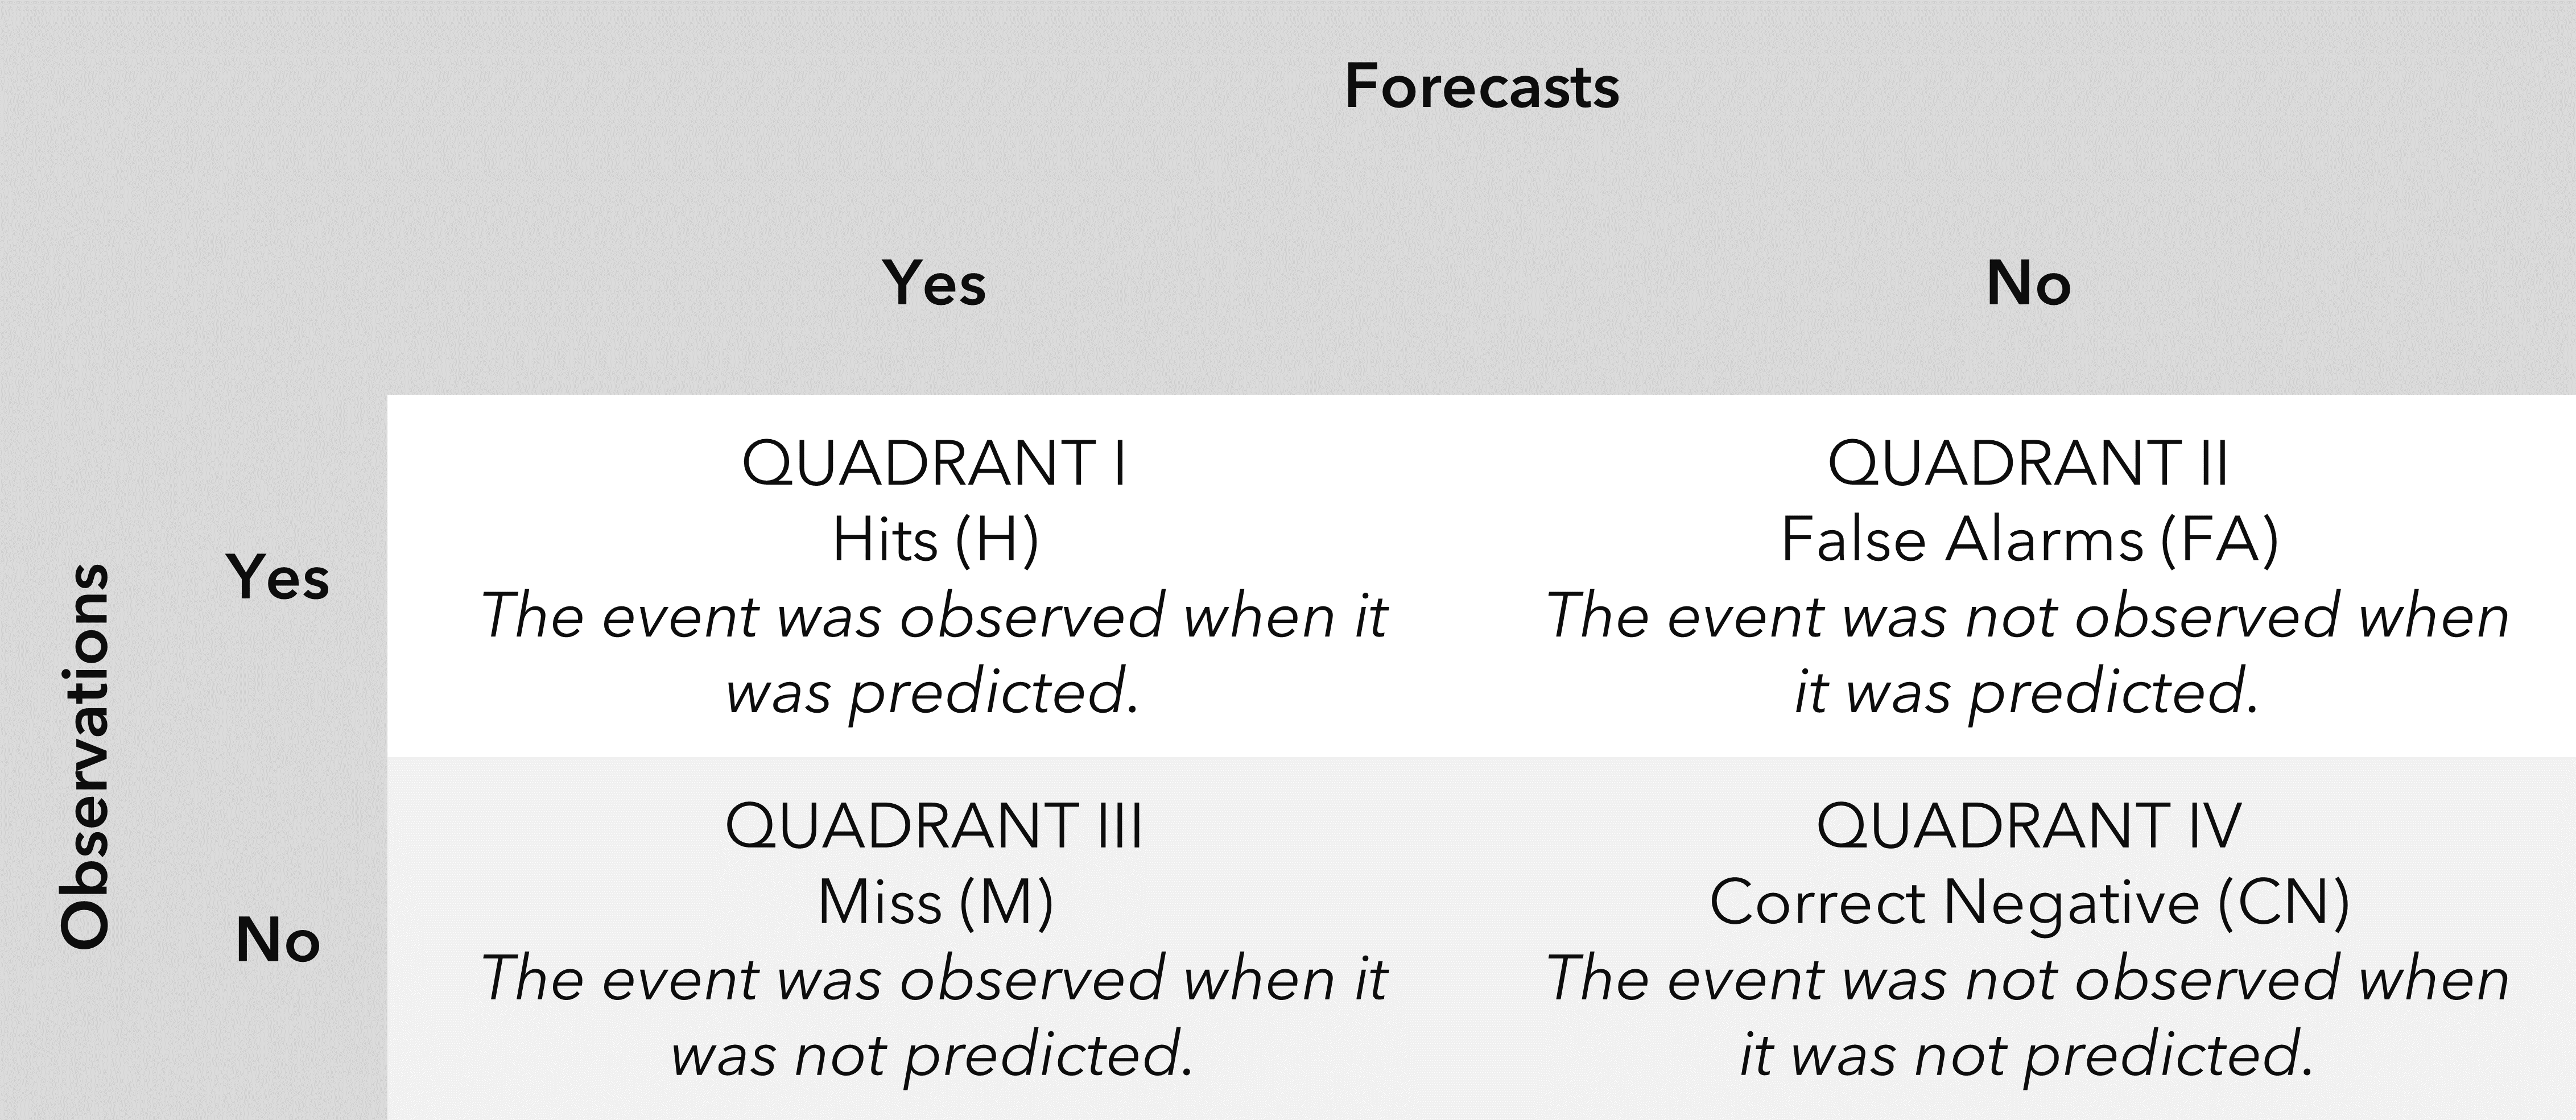
\includegraphics[width=\textwidth]{contingency_table.png}
\label{table:contingency_table}
\end{table}

Relative Operating Characteristic (ROC) curves are built from 2x2 contingency tables (Table \ref{contingency_table}), quantifying hits (H) misses (M), false alarms (FA), and correct negatives (CN). Hit rates (HR) and false alarm rates (FAR) are computed, respectively, from equations \ref{eq:hr} and \ref{eq:far}:

\begin{equation}
\mathrm{HR} = \frac{\mathrm{H}}{\mathrm{H} + \mathrm{M}}\quad[\text{values between }0\text{ and }1]
\label{eq:hr}
\end{equation}

\begin{equation}
\mathrm{FAR} = \frac{\mathrm{FA}}{\mathrm{FA} + \mathrm{CN}}\quad[\text{values between }0\text{ and }1]
\label{eq:far}
\end{equation}

HRs are mapped (Y-axis) against FARs (X-axis) in a unit square. The form of the ROC curve shows how HRs vary with FARs as one systematically lowers the thresholds probability at which it is assumed that an event has technically been forecast to happen (i.e. 100\% of probability the bottom left corner to 0\% probability at the top right corner). The values of the geometrical area under the ROC curve (AROC) provide a summary measure of the discrimination ability across all probability thresholds. The plot of AROC values for different lead times allows us to compare the discrimination ability between the rainfall-based predictions of areas at risk of flash floods, and the multi-parameter-based, data-driven predictions, (both at short- and medium-range lead times). Perfect discrimination is obtained when only HRs grow and FARs remain zero. It is represented by a ROC curve that rises along the Y-axis from the bottom left corner of the unit square to the top-left corner and moves straight to the top-right corner. In this case, the AROC is equal to 1. If HRs and FARs grow at the same rate, the forecasts have no discrimination ability (as a climatological forecast). In this case, the ROC curve lies along the diagonal and AROC equals 0.5. 

\begin{figure}[htbp]
\centering
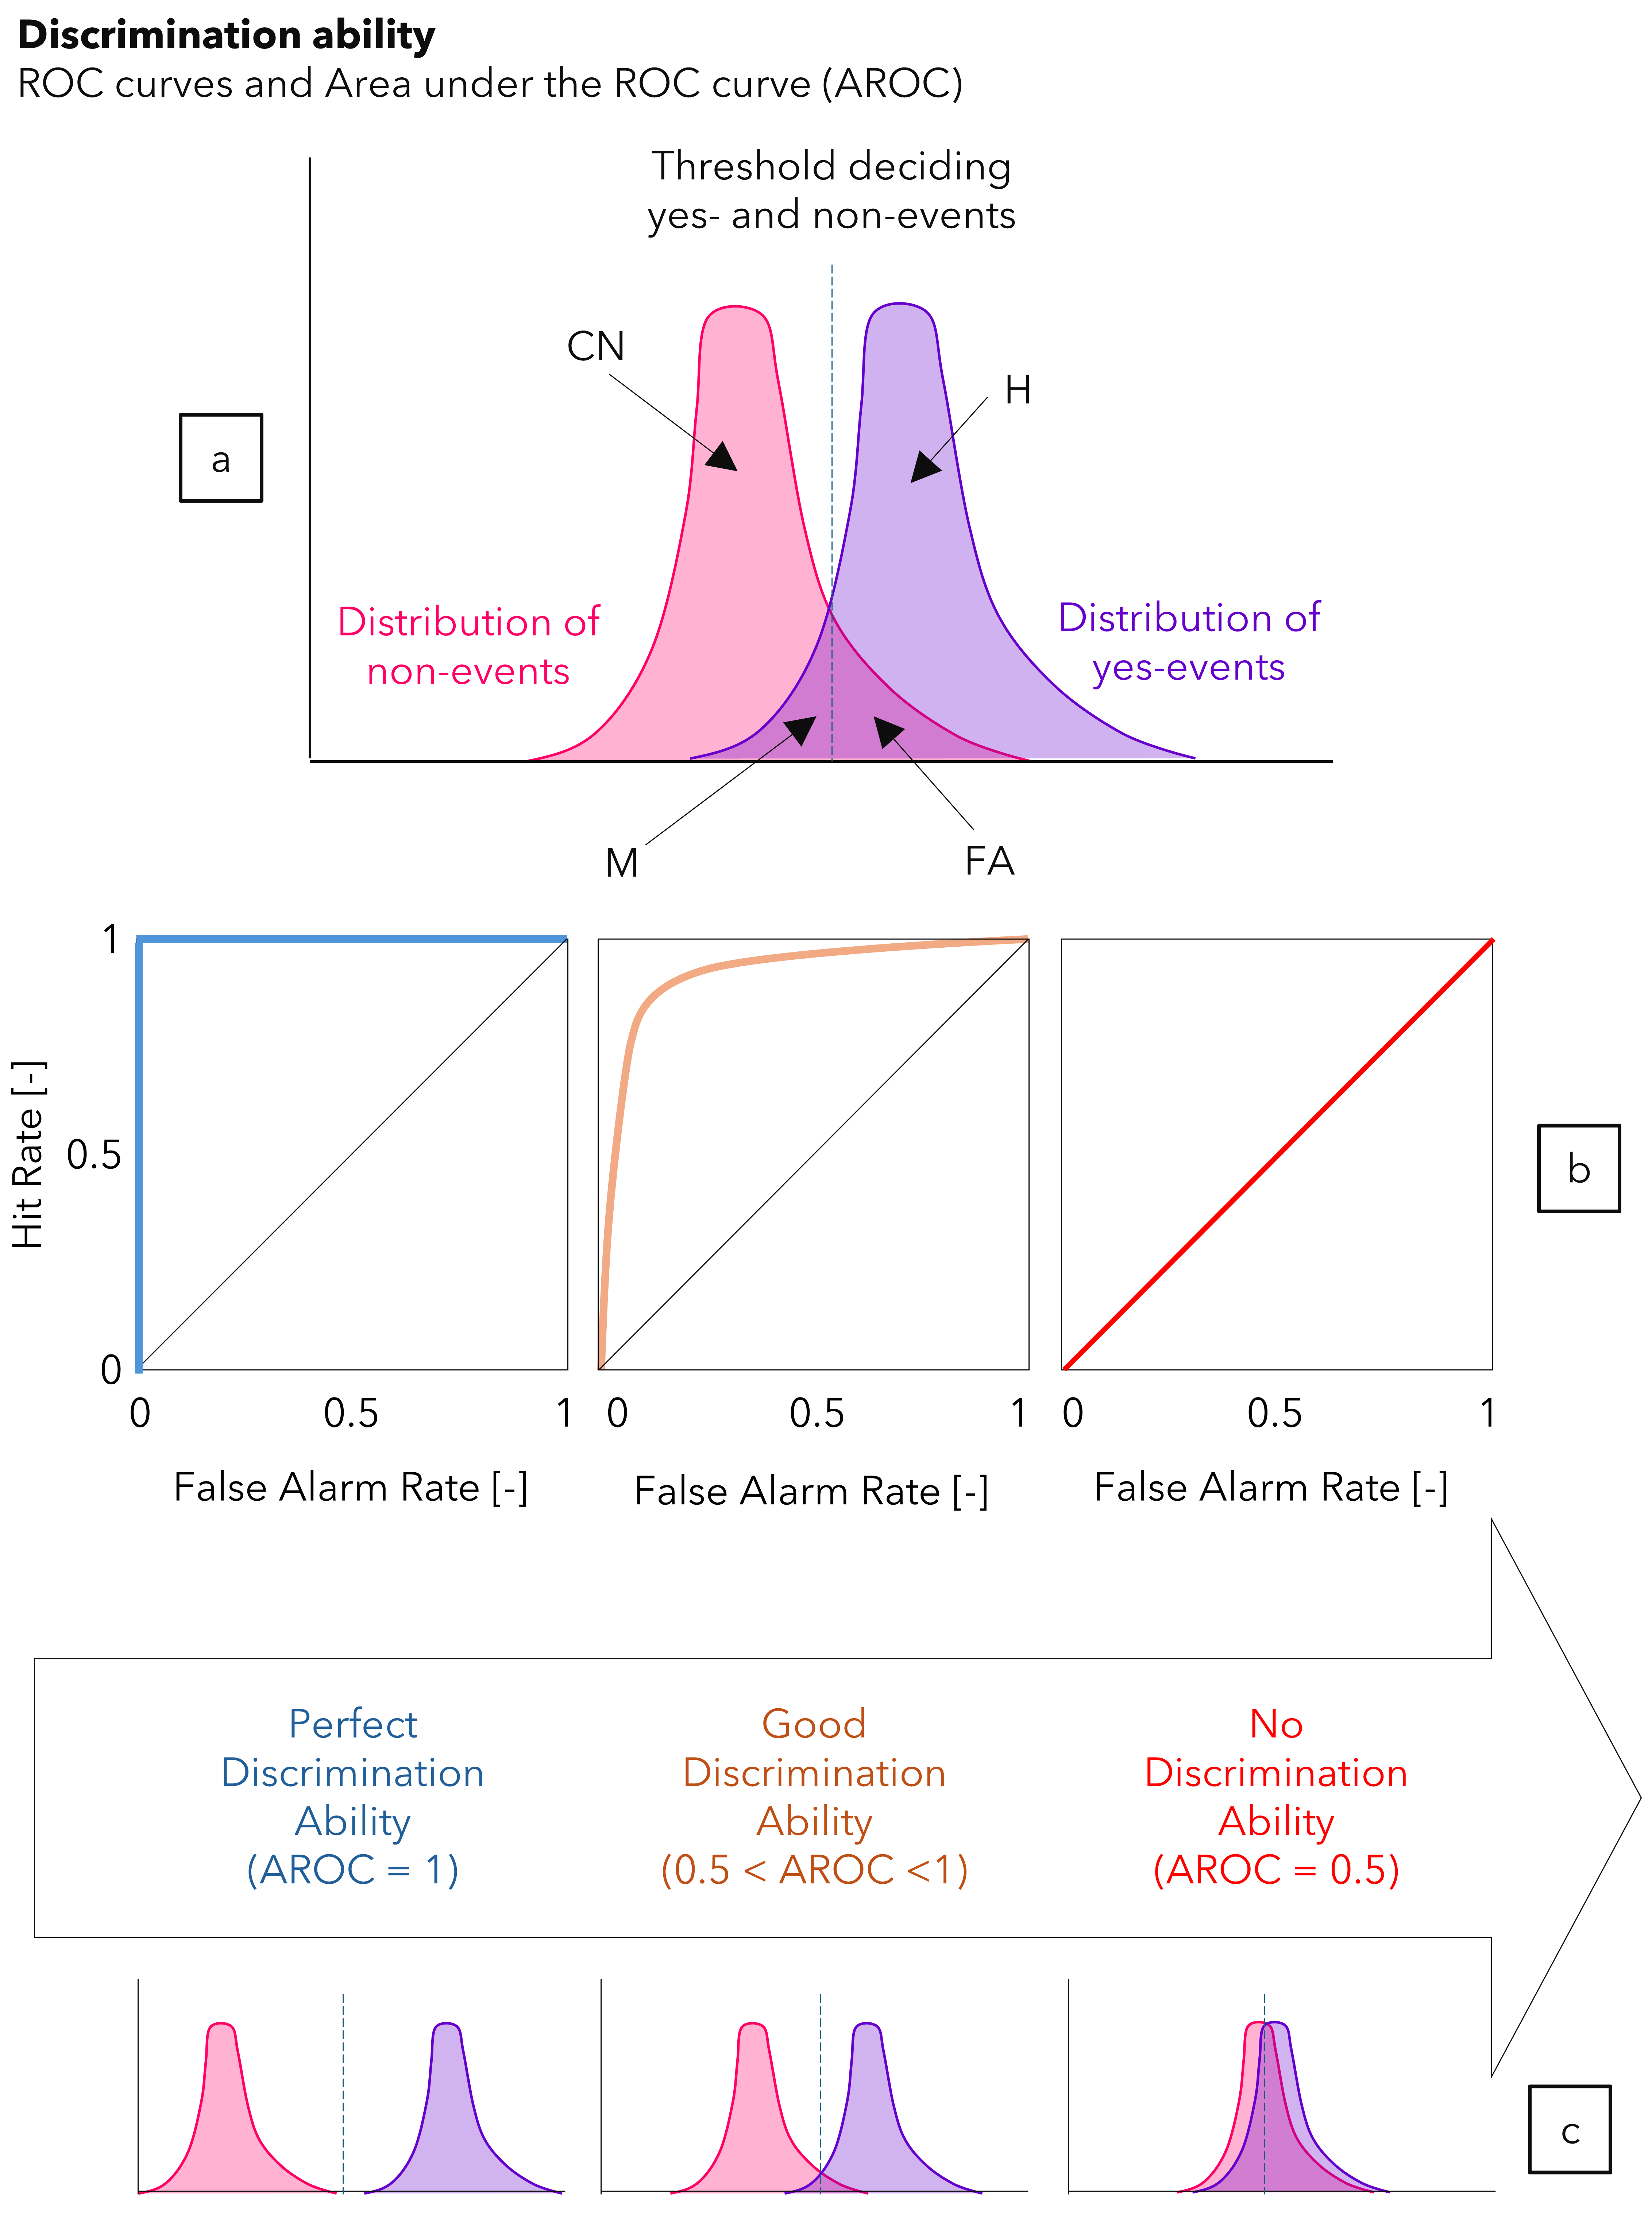
\includegraphics[width=\textwidth]{roc_examples.png}
\caption{\textbf{Discrimination ability of forecasts.} Examples of how ROC curves look like for different degrees of forecast's discrimination ability.}
\label{fig:roc_examples}
\end{figure}

How ROC curves and AROCs are computed can impact the interpretation of forecasts discrimination ability. For rainfall-based predictions, the ROC curves will be built for incremental decision thresholds that are materially assessable from the real ensemble configuration. In this way, we can estimate the "real" forecast discrimination ability \citep{wilks_statistical_2020}. Probability thresholds are determined by considering the full discretisation ability in the ensemble (e.g., 99 members in the case of ERA5-ecPoint). This ensures that the ROC curves are as complete as possible \citep{Bouallegue_2022}. The number of thresholds corresponds, therefore, to the number of members exceeding the verifying rainfall threshold so that for an enmble of size M, maximum discretisation is achieved by M+1 probability thresholds (i.e., 0, 1/M, 2/M, ...., M/M=1). For the data-driven forecasts, where the forecast probability is provided by the model with continuous numbers between 0 and 1, the decision (probability) thresholds are defined by the user. In this thesis, a discretisation of 0.01 (equivalent to 1\%) and 0.001 (equivalent to 0.1\%) will be considered given the low frequency observed of flash flood events in the observational database. The ROC curve is then built by straight segments joining successive points. It is then completed by joining that last meaningful point with a straight line in the top-rigth corner of the unit square. For rare events, the points of a ROC curve cluster in the graph's bottom left corner and completing the ROC with a straight line might give the impression that part of the curve is missing \citep{Casati_2008}. How much the curve appears incomplete depends on the ensemble size and the base rate of the event. The area under the ROC curve (AROC) will be computed using a trapezoidal approximation by adding the areas of single trapeziums formed by the straight lines between consecutive points in the ROC curve \citep{Bouallegue_2022}. 

From what written before, the ROC curves represent the breakdown measure of discrimination ability as it will be possible to examine the values of HRs and FARs at different decision (probability) thresholds. AROC will represent instead the overall measure of discrimination ability.

%%%%%%%%%%%%%%%%%
\section{Results}
\label{flash_flood_focused_verification_rainfall_based_ff_RESULTS}

%%%%%%%%%
\subsection{Assessment of rainfall-based predictions of areas at risk of flash floods}
\label{verif_rainfall_based_fc}

\subsubsection{Overall verification scores: frequency bias and area under the ROC curve}

\begin{figure}[htbp]
\centering
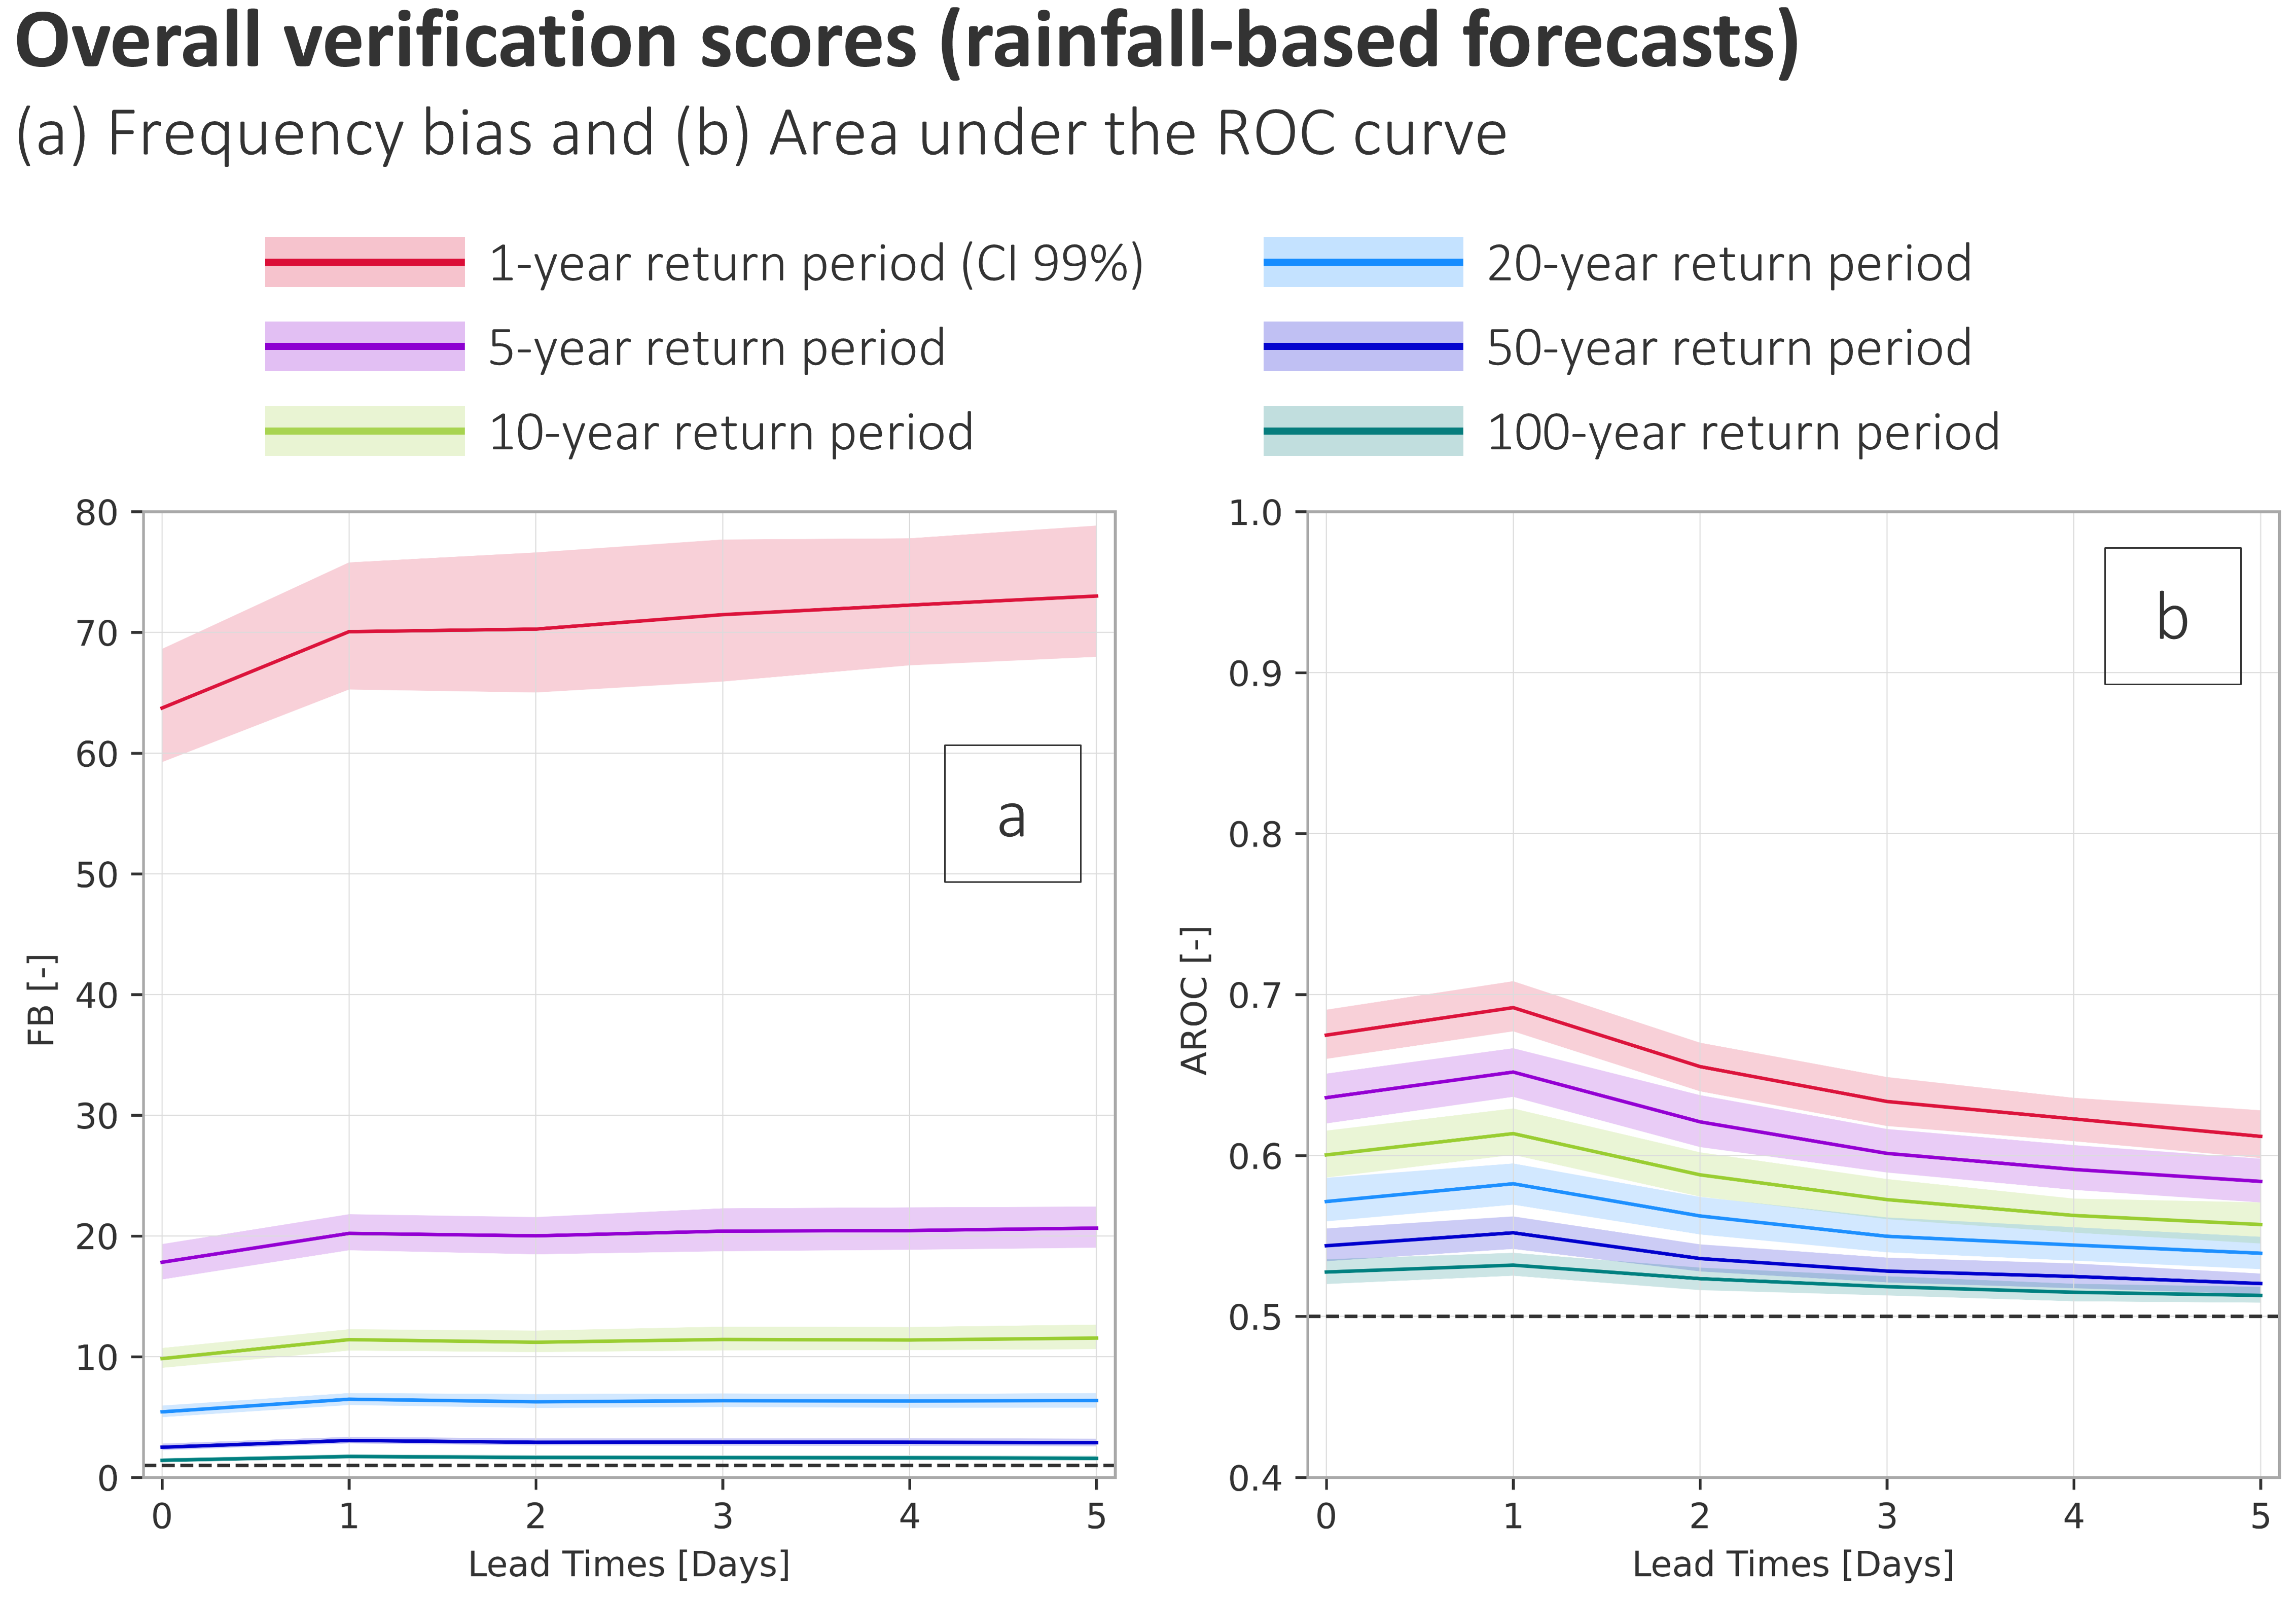
\includegraphics[width=\textwidth]{chapter_05/figures/rainfall_based_ff_verif_overall_scores.png}
\caption{\textbf{Overall verification scores for the rainfall-based forecasts of areas at risk of flash flood.} Panel (a) shows the frequency bias (solid lines) for 1-year (in red), 5-year (in purple), 10-year (in light green), 20-year (in cyan), 50-year (in blue), and 100-year return period (in green). The corresponding shaded areas represent the confidence intervals at 99\% confidence level. The inset box contains a zoomed-in version of the panel to show better the frequency bias values close to 1 (representing perfect bias). Panel (b) shows the area under the ROC curve.}
\label{fig:rainfall_based_ff_verif_overall_scores}
\end{figure}


\subsubsection{Discrimination ability}

All forecasts for rainfall events exceeding the 1-year return period threshold (Figure \ref{fig:rainfall_based_ff_verif_breakdown_scores_roc_1rp}) exhibit a discrimination ability superior to random chance, as the curves are above the diagonal reference line. A systematic degradation in discrimination ability is observed with increasing lead time, with the Area Under the ROC Curve (AROC) values ranging from 0.675 for the short-range forecasts (Figure \ref{fig:rainfall_based_ff_verif_breakdown_scores_roc_1rp}a) to 0.612 (\sim9\% reduction) for t+120 (day 5, Figure \ref{fig:rainfall_based_ff_verif_breakdown_scores_roc_1rp}f). Despite such a reduction, the forecasts show a good discrimination ability throughout the forecast horizon. Day 1 forecasts (t+24) show a higher discrimination ability than the short-range forecasts, and only from day 2 forecasts (t+48), the discrimination ability of the long-range forecasts goes below that of the reanalysis. The relatively narrow confidence intervals (at 99\% confidence level) suggest that the differences in skill between forecast configurations are statistically meaningful at the considered confidence level.

\begin{figure}[htbp]
\centering
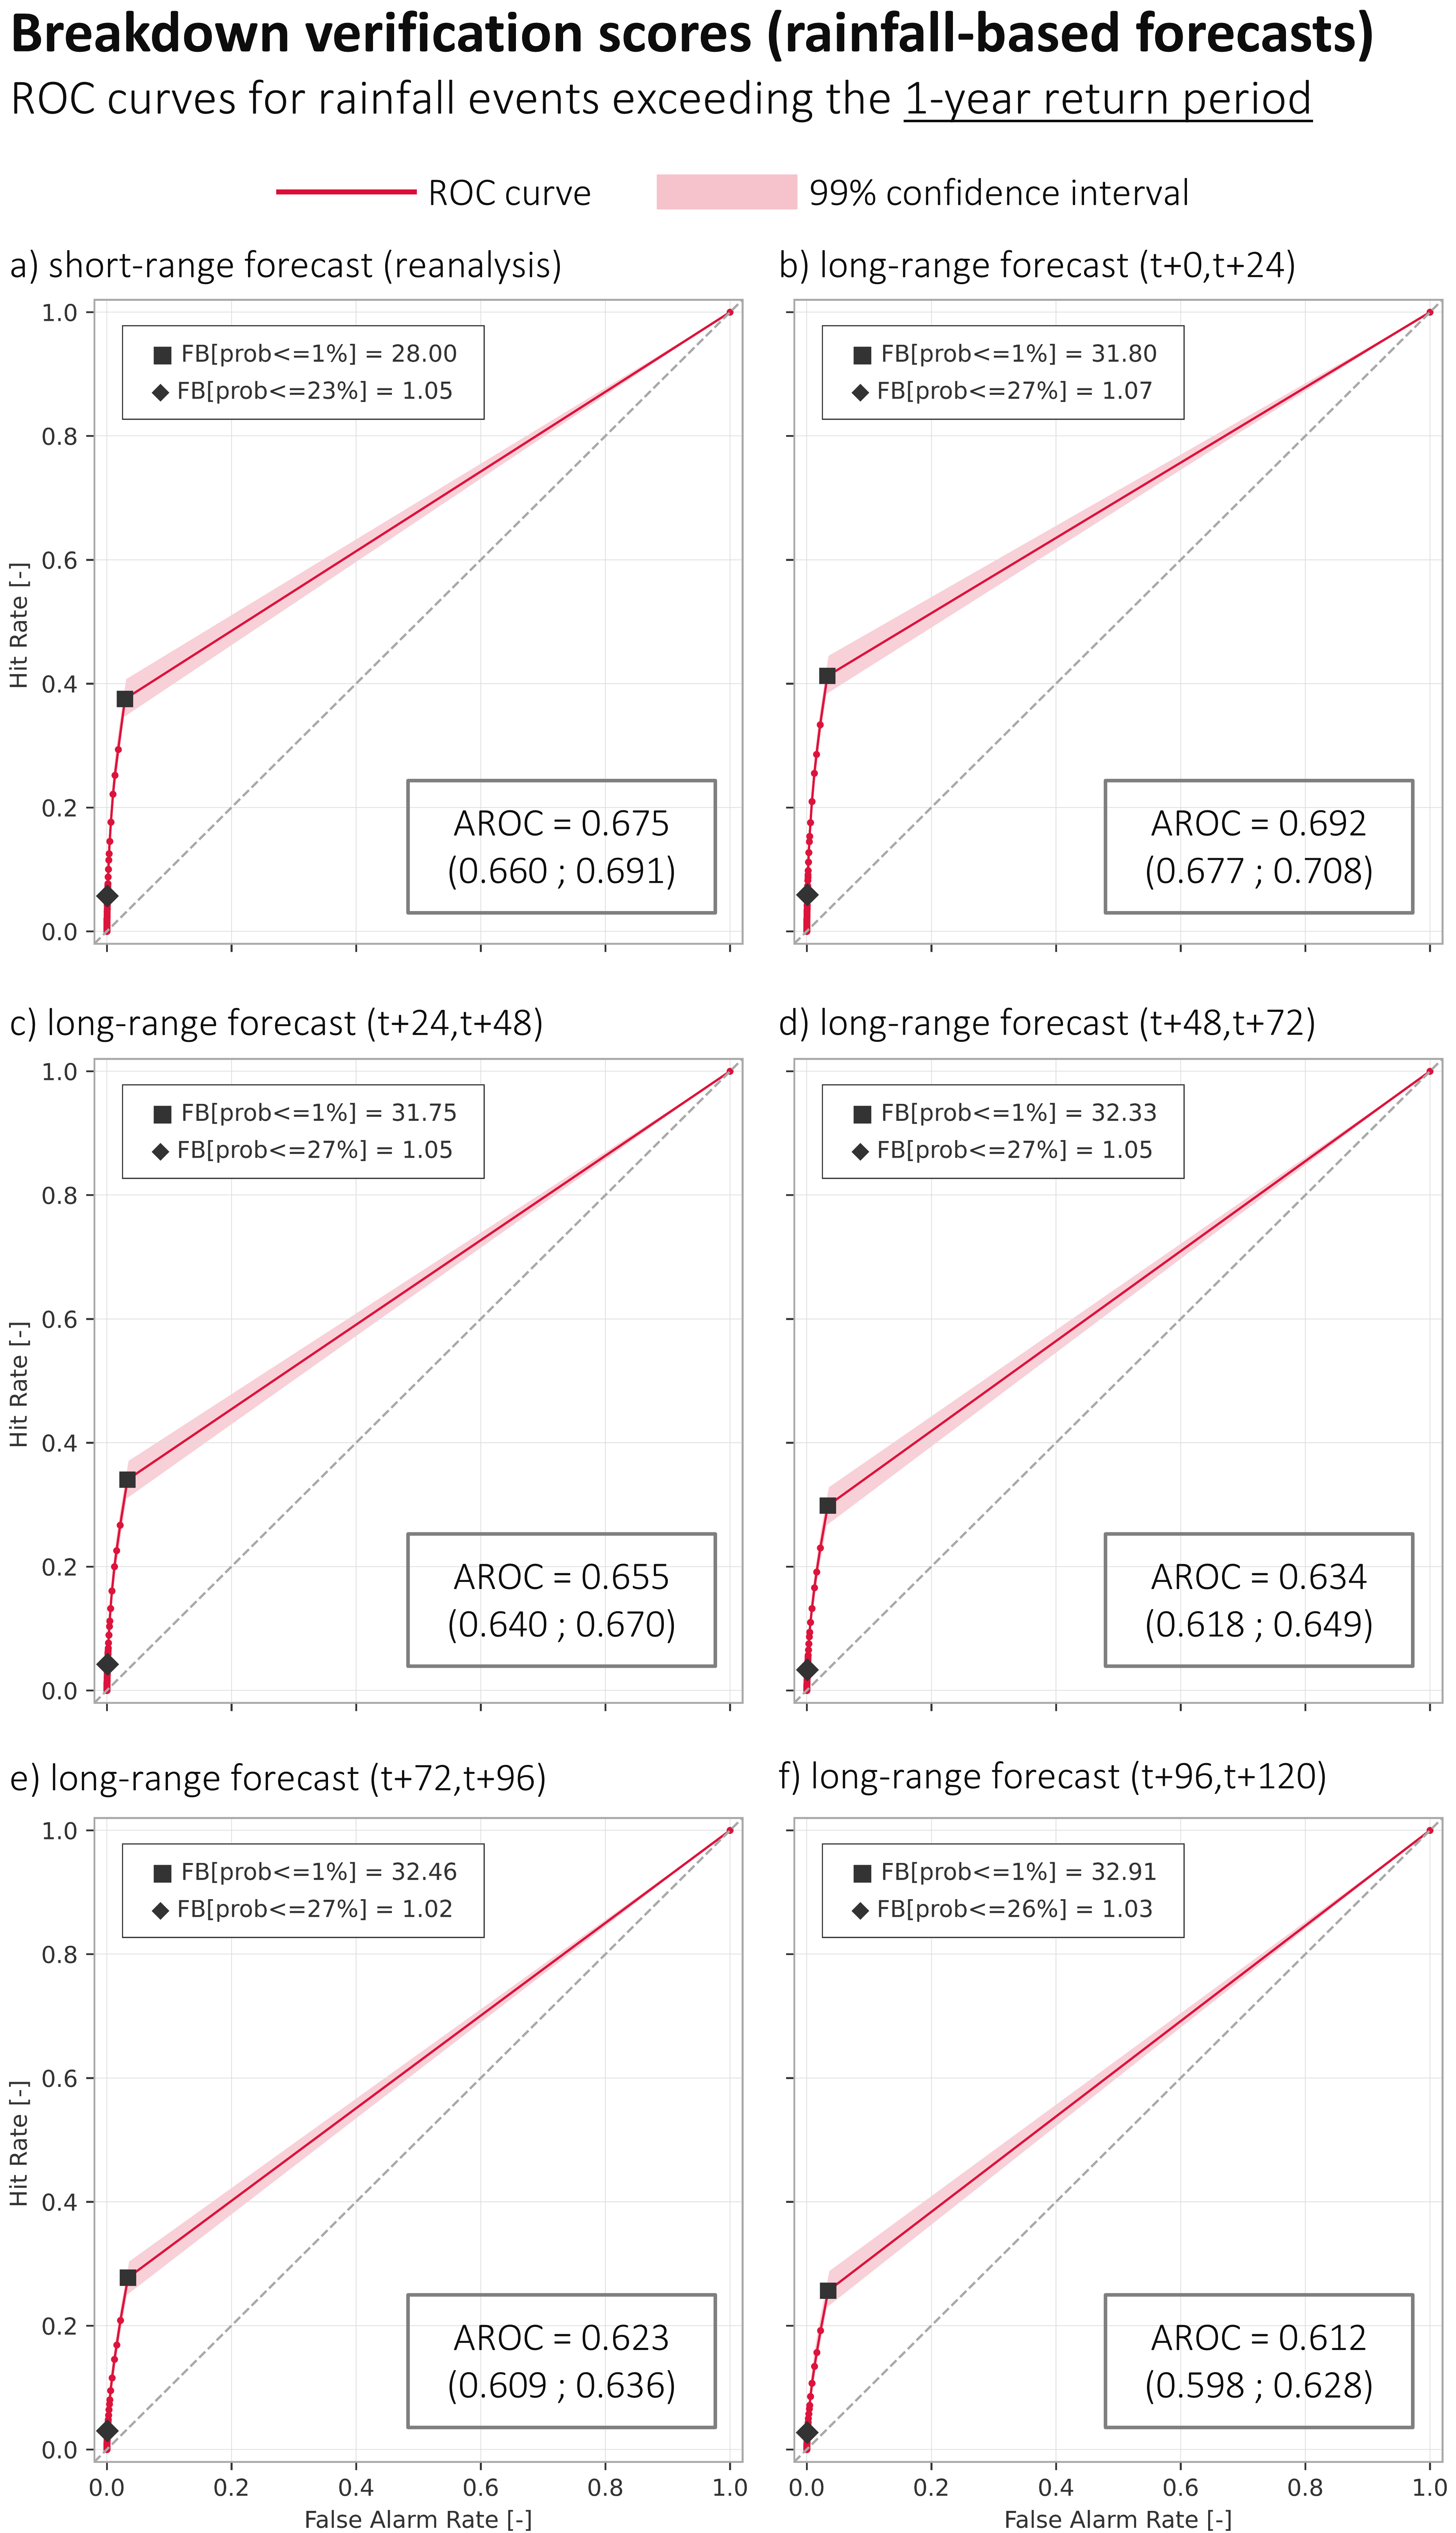
\includegraphics[width=\textwidth]{chapter_05/figures/rainfall_based_ff_verif_breakdown_scores_roc_1rp.png}
\caption{\textbf{ROC curves for tp >= 1-year return period for the rainfall-based forecasts of areas at risk of flash floods built with ERA5-ecPoint.} Panel (a) shows the ROC curve (blue solid line) for the short-range predictions together with the confidence intervals (blue shaded area) at 99\% confidence level. Panels (b) to (f) refer to the long-range forecasts, for accumulation periods ending in t+24, t+48, t+72, t+96, and t+120, respectively. The pink dots refer to the probability threshold at which the frequency bias has the closest value to 1 (i.e., perfectly reliable forecast), while the orange dot shows the value of the frequency bias for the lowest probability threshold available in ERA5-ecPoint (i.e., the 99th percentile).}
\label{fig:rainfall_based_ff_verif_breakdown_scores_roc_1rp}
\end{figure}

The pink dot in Figure \ref{fig:rainfall_based_ff_verif_breakdown_scores_roc_1rp}a shows that perfect reliability (i.e. frequency bias equal to 1) is reach for probabilities <= 23\%. For the long-range forecasts, the probability thresholds at which perfect reliability is achieved is compatible to the short-range, being 27\% for all the lead times except t+120 which is 26\%. The frequency bias for the lowest probability threshold (i.e. 99th percentile or probability threshold equal to 1\%) in the short-range forecasts equals to 28. The frequency biases for the long-range forecasts are similar, falling between 31 and 33. 

Similar results are obtained for the 5-, 10-, 20-, 50-, and 100-year return periods.

\begin{figure}[htbp]
\centering
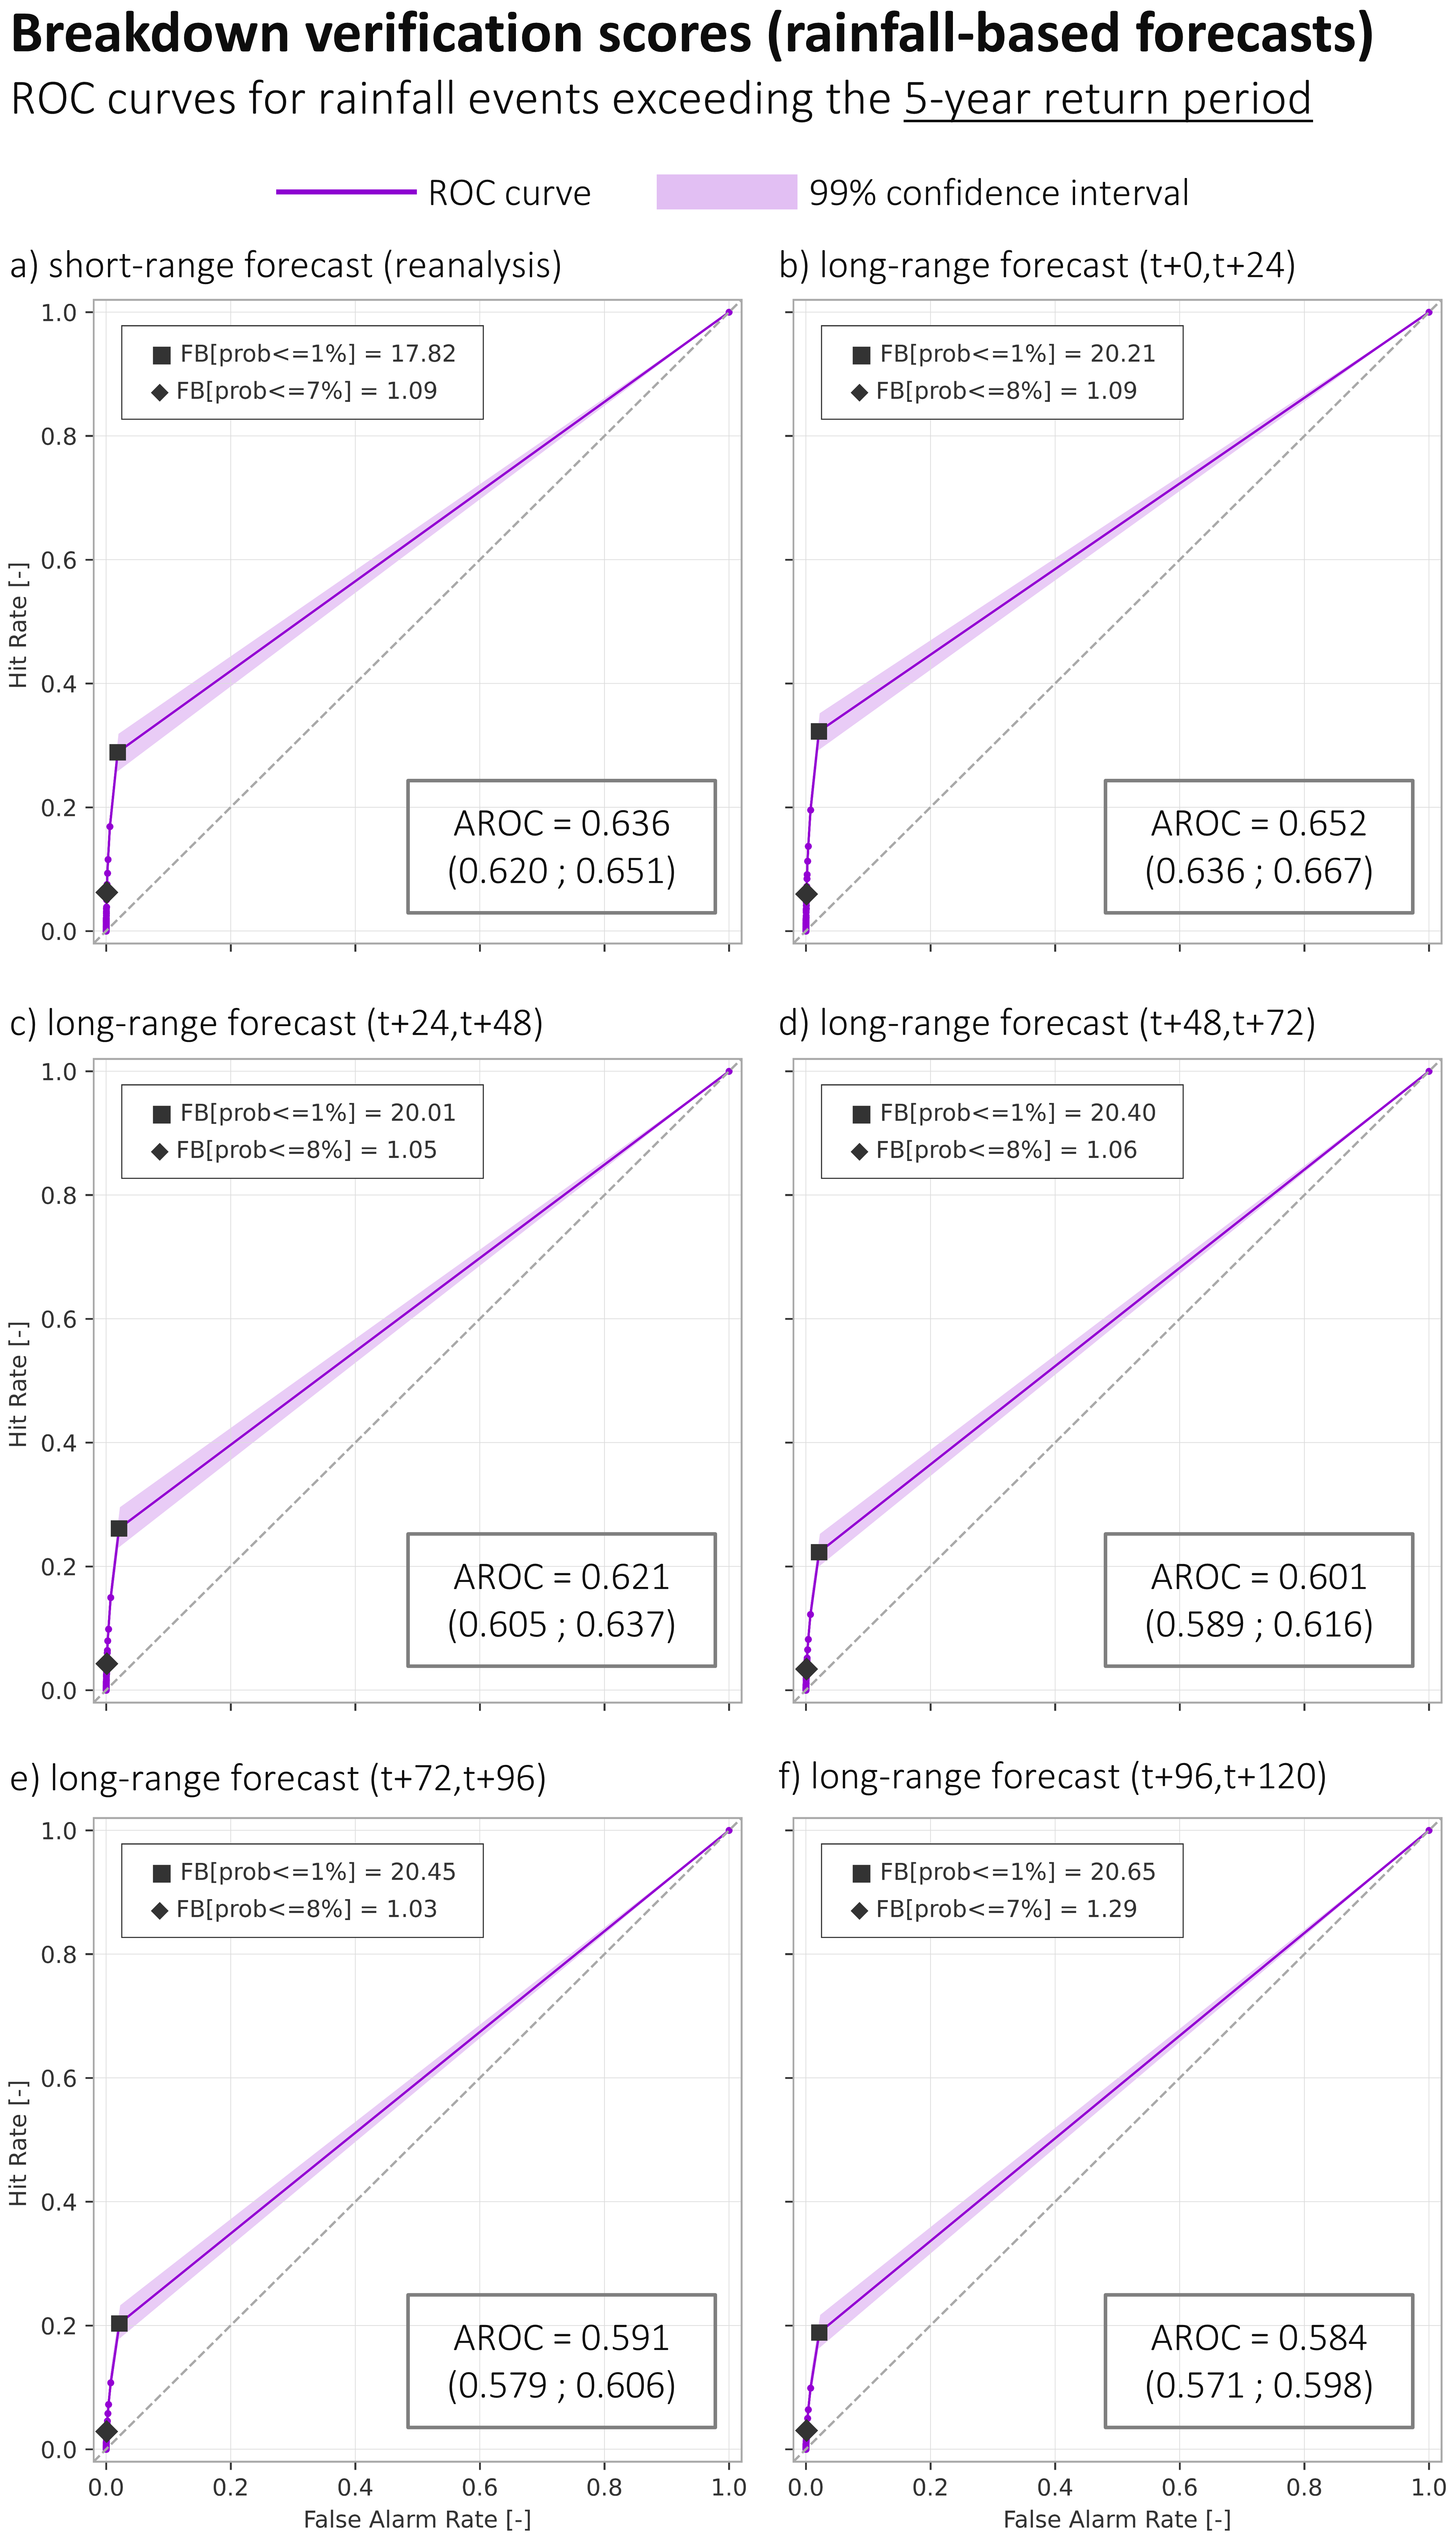
\includegraphics[width=\textwidth]{chapter_05/figures/rainfall_based_ff_verif_breakdown_scores_roc_5rp.png}
\caption{\textbf{ROC curves for tp >= 5-year return period for the rainfall-based forecasts of areas at risk of flash floods built with ERA5-ecPoint.} Similar to Figure \ref{fig:rainfall_based_ff_verif_breakdown_scores_roc_1rp}.}
\label{fig:rainfall_based_ff_verif_breakdown_scores_roc_5rp}
\end{figure}

\begin{figure}[htbp]
\centering
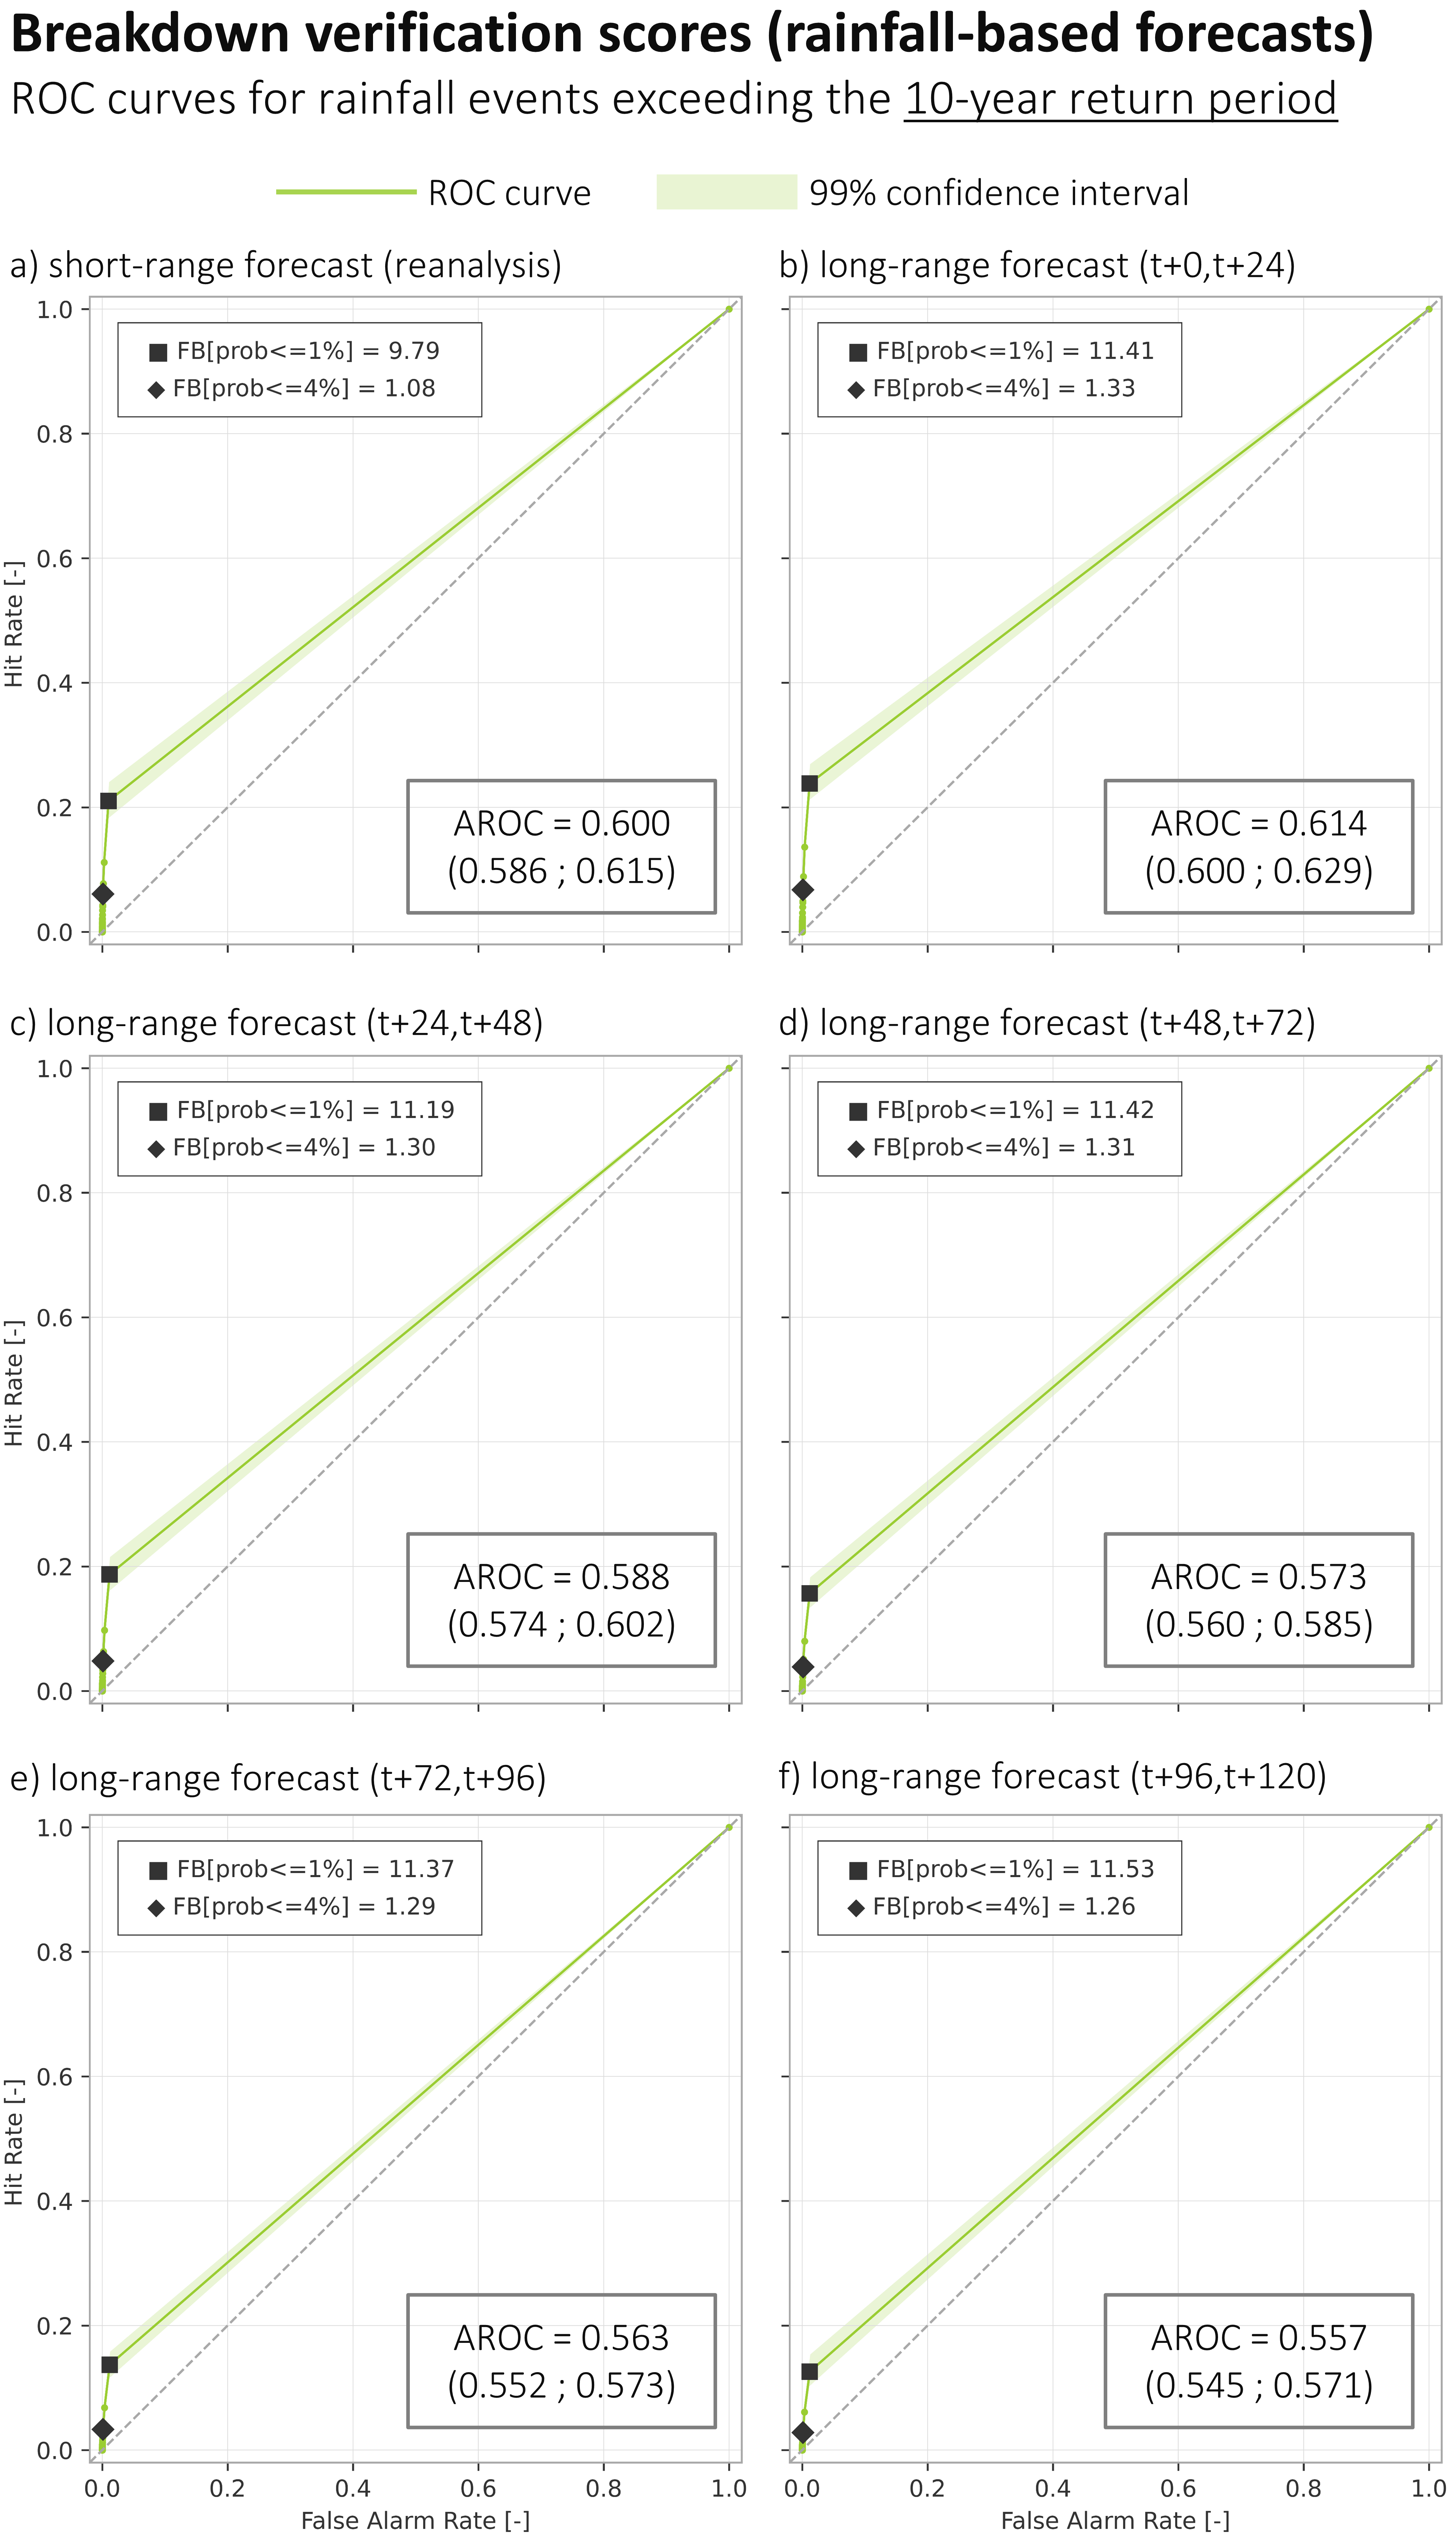
\includegraphics[width=\textwidth]{chapter_05/figures/rainfall_based_ff_verif_breakdown_scores_roc_10rp.png}
\caption{\textbf{ROC curves for tp >= 10-year return period for the rainfall-based forecasts of areas at risk of flash floods built with ERA5-ecPoint.} Similar to Figure \ref{fig:rainfall_based_ff_verif_breakdown_scores_roc_1rp}.}
\label{fig:rainfall_based_ff_verif_breakdown_scores_roc_10rp}
\end{figure}

\begin{figure}[htbp]
\centering
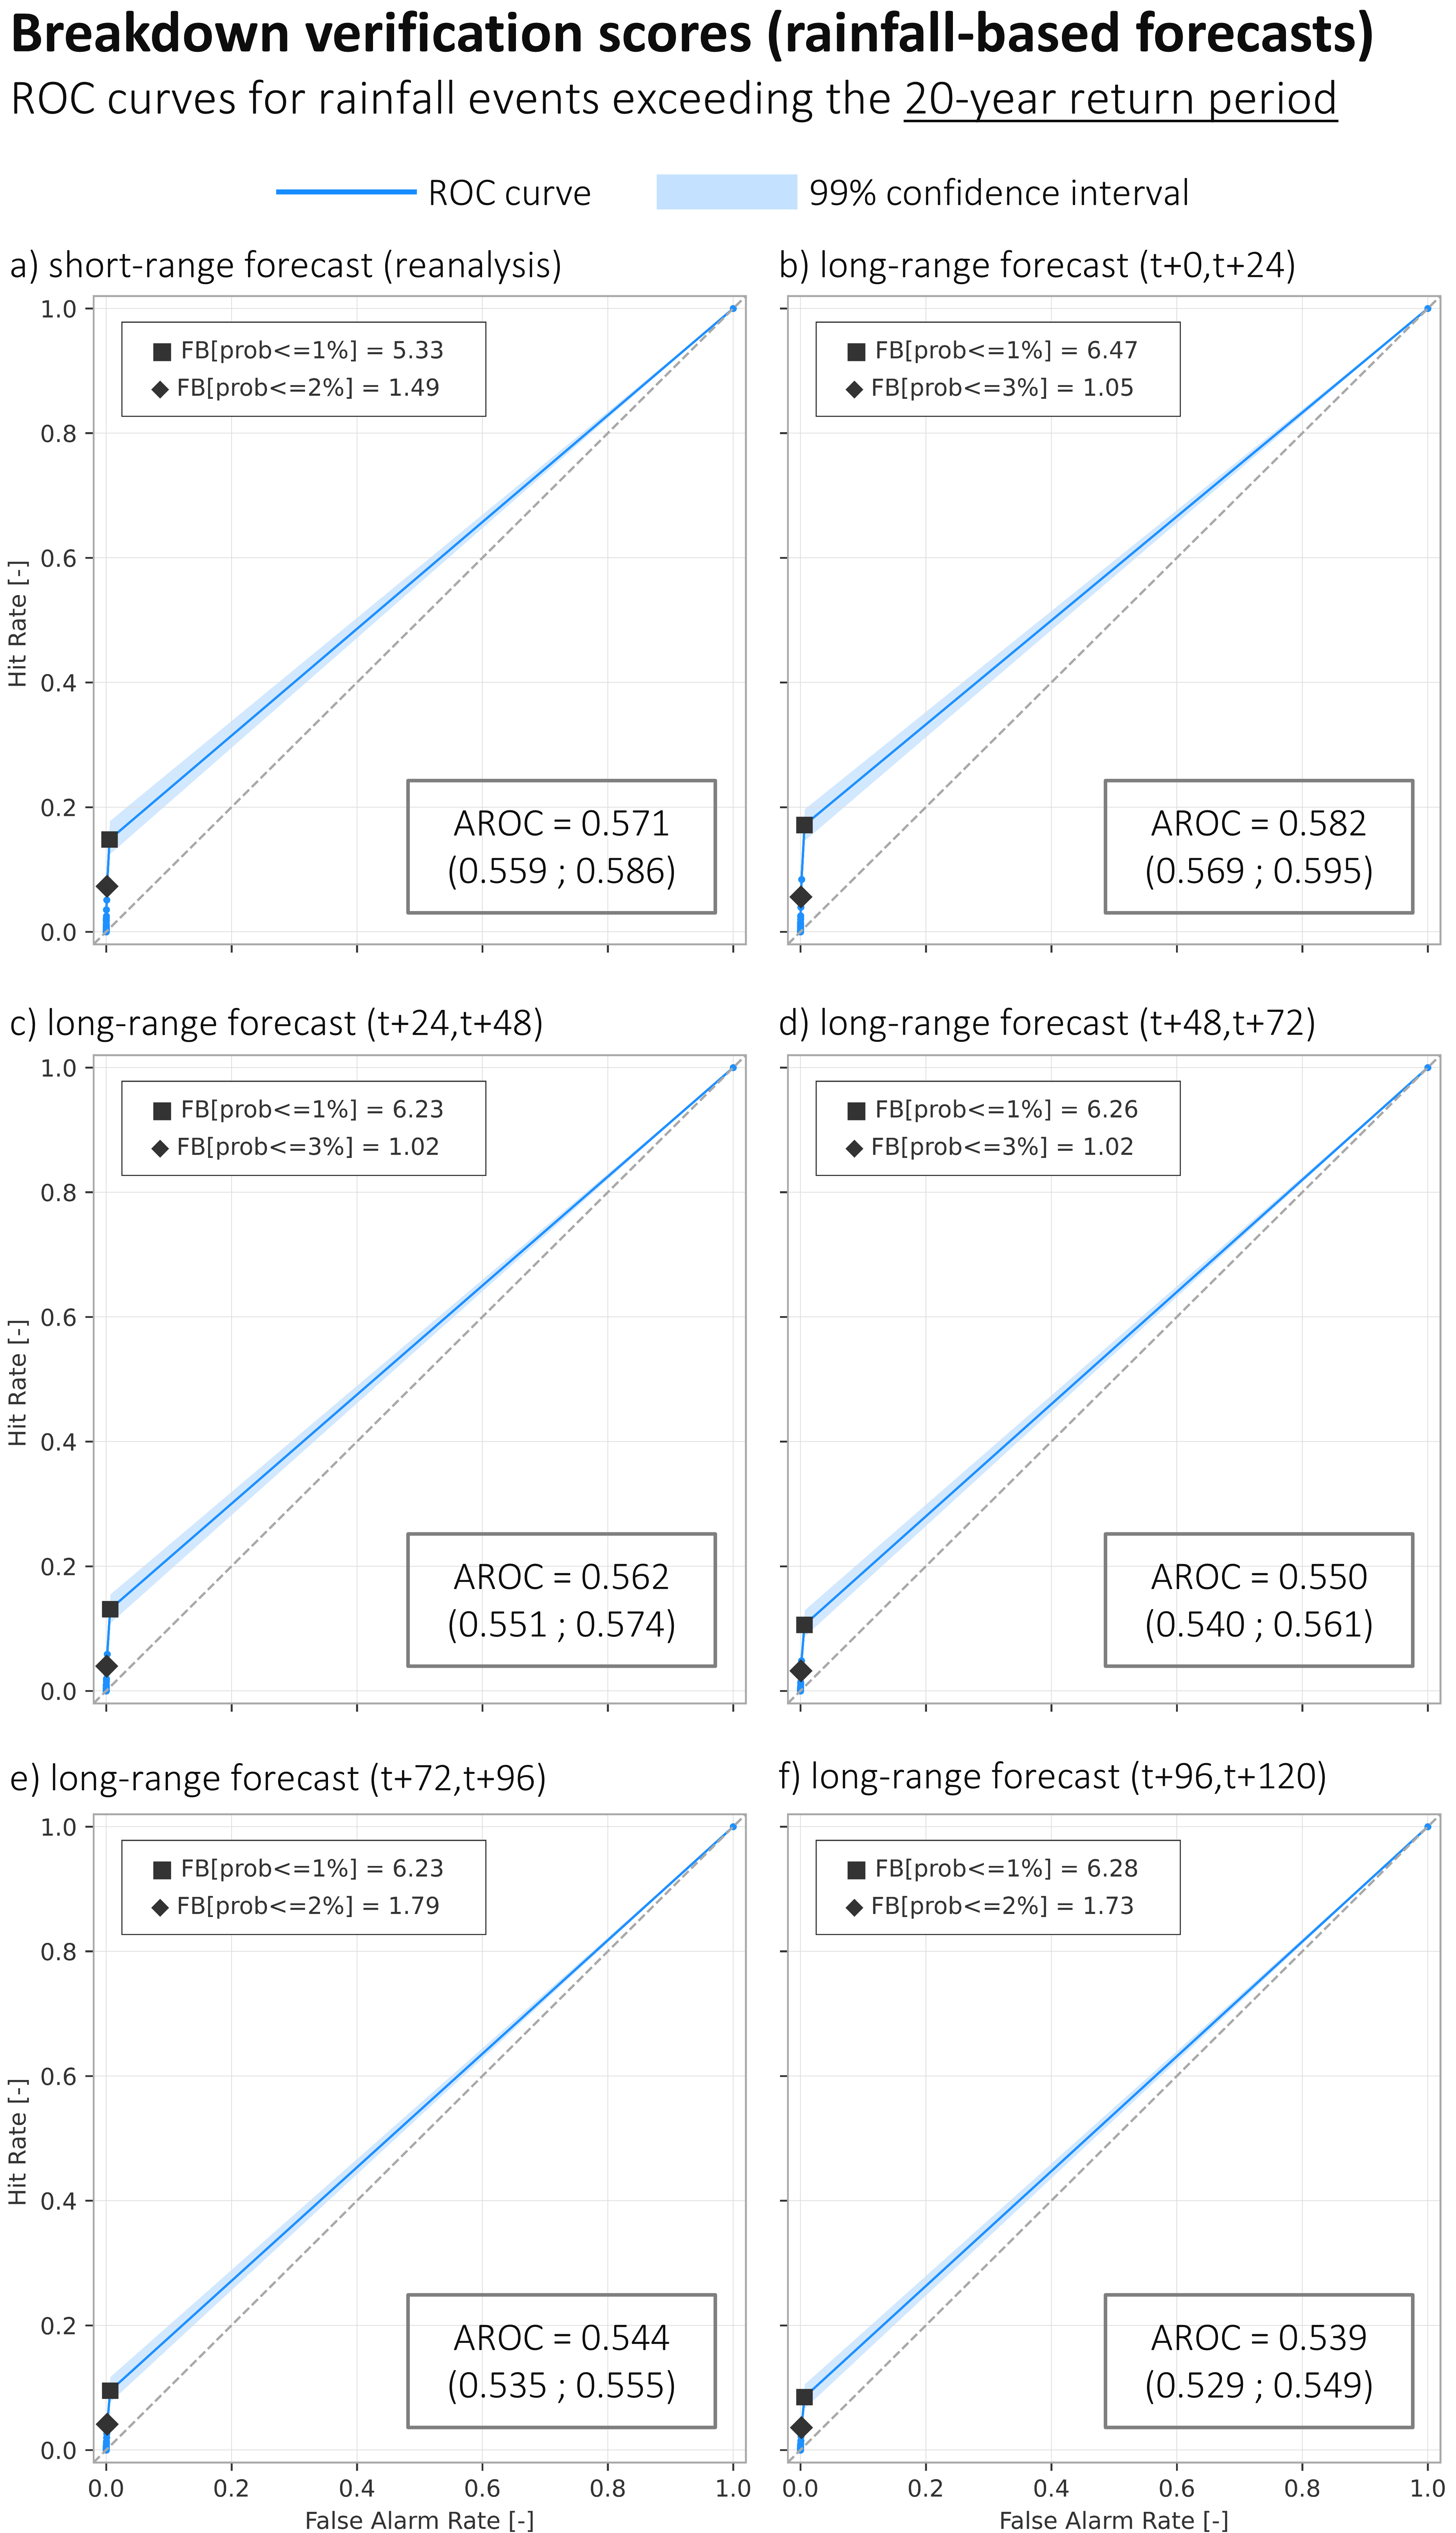
\includegraphics[width=\textwidth]{chapter_05/figures/rainfall_based_ff_verif_breakdown_scores_roc_20rp.png}
\caption{\textbf{ROC curves for tp >= 20-year return period for the rainfall-based forecasts of areas at risk of flash floods built with ERA5-ecPoint.} Similar to Figure \ref{fig:rainfall_based_ff_verif_breakdown_scores_roc_1rp}.}
\label{fig:rainfall_based_ff_verif_breakdown_scores_roc_20rp}
\end{figure}

\begin{figure}[htbp]
\centering
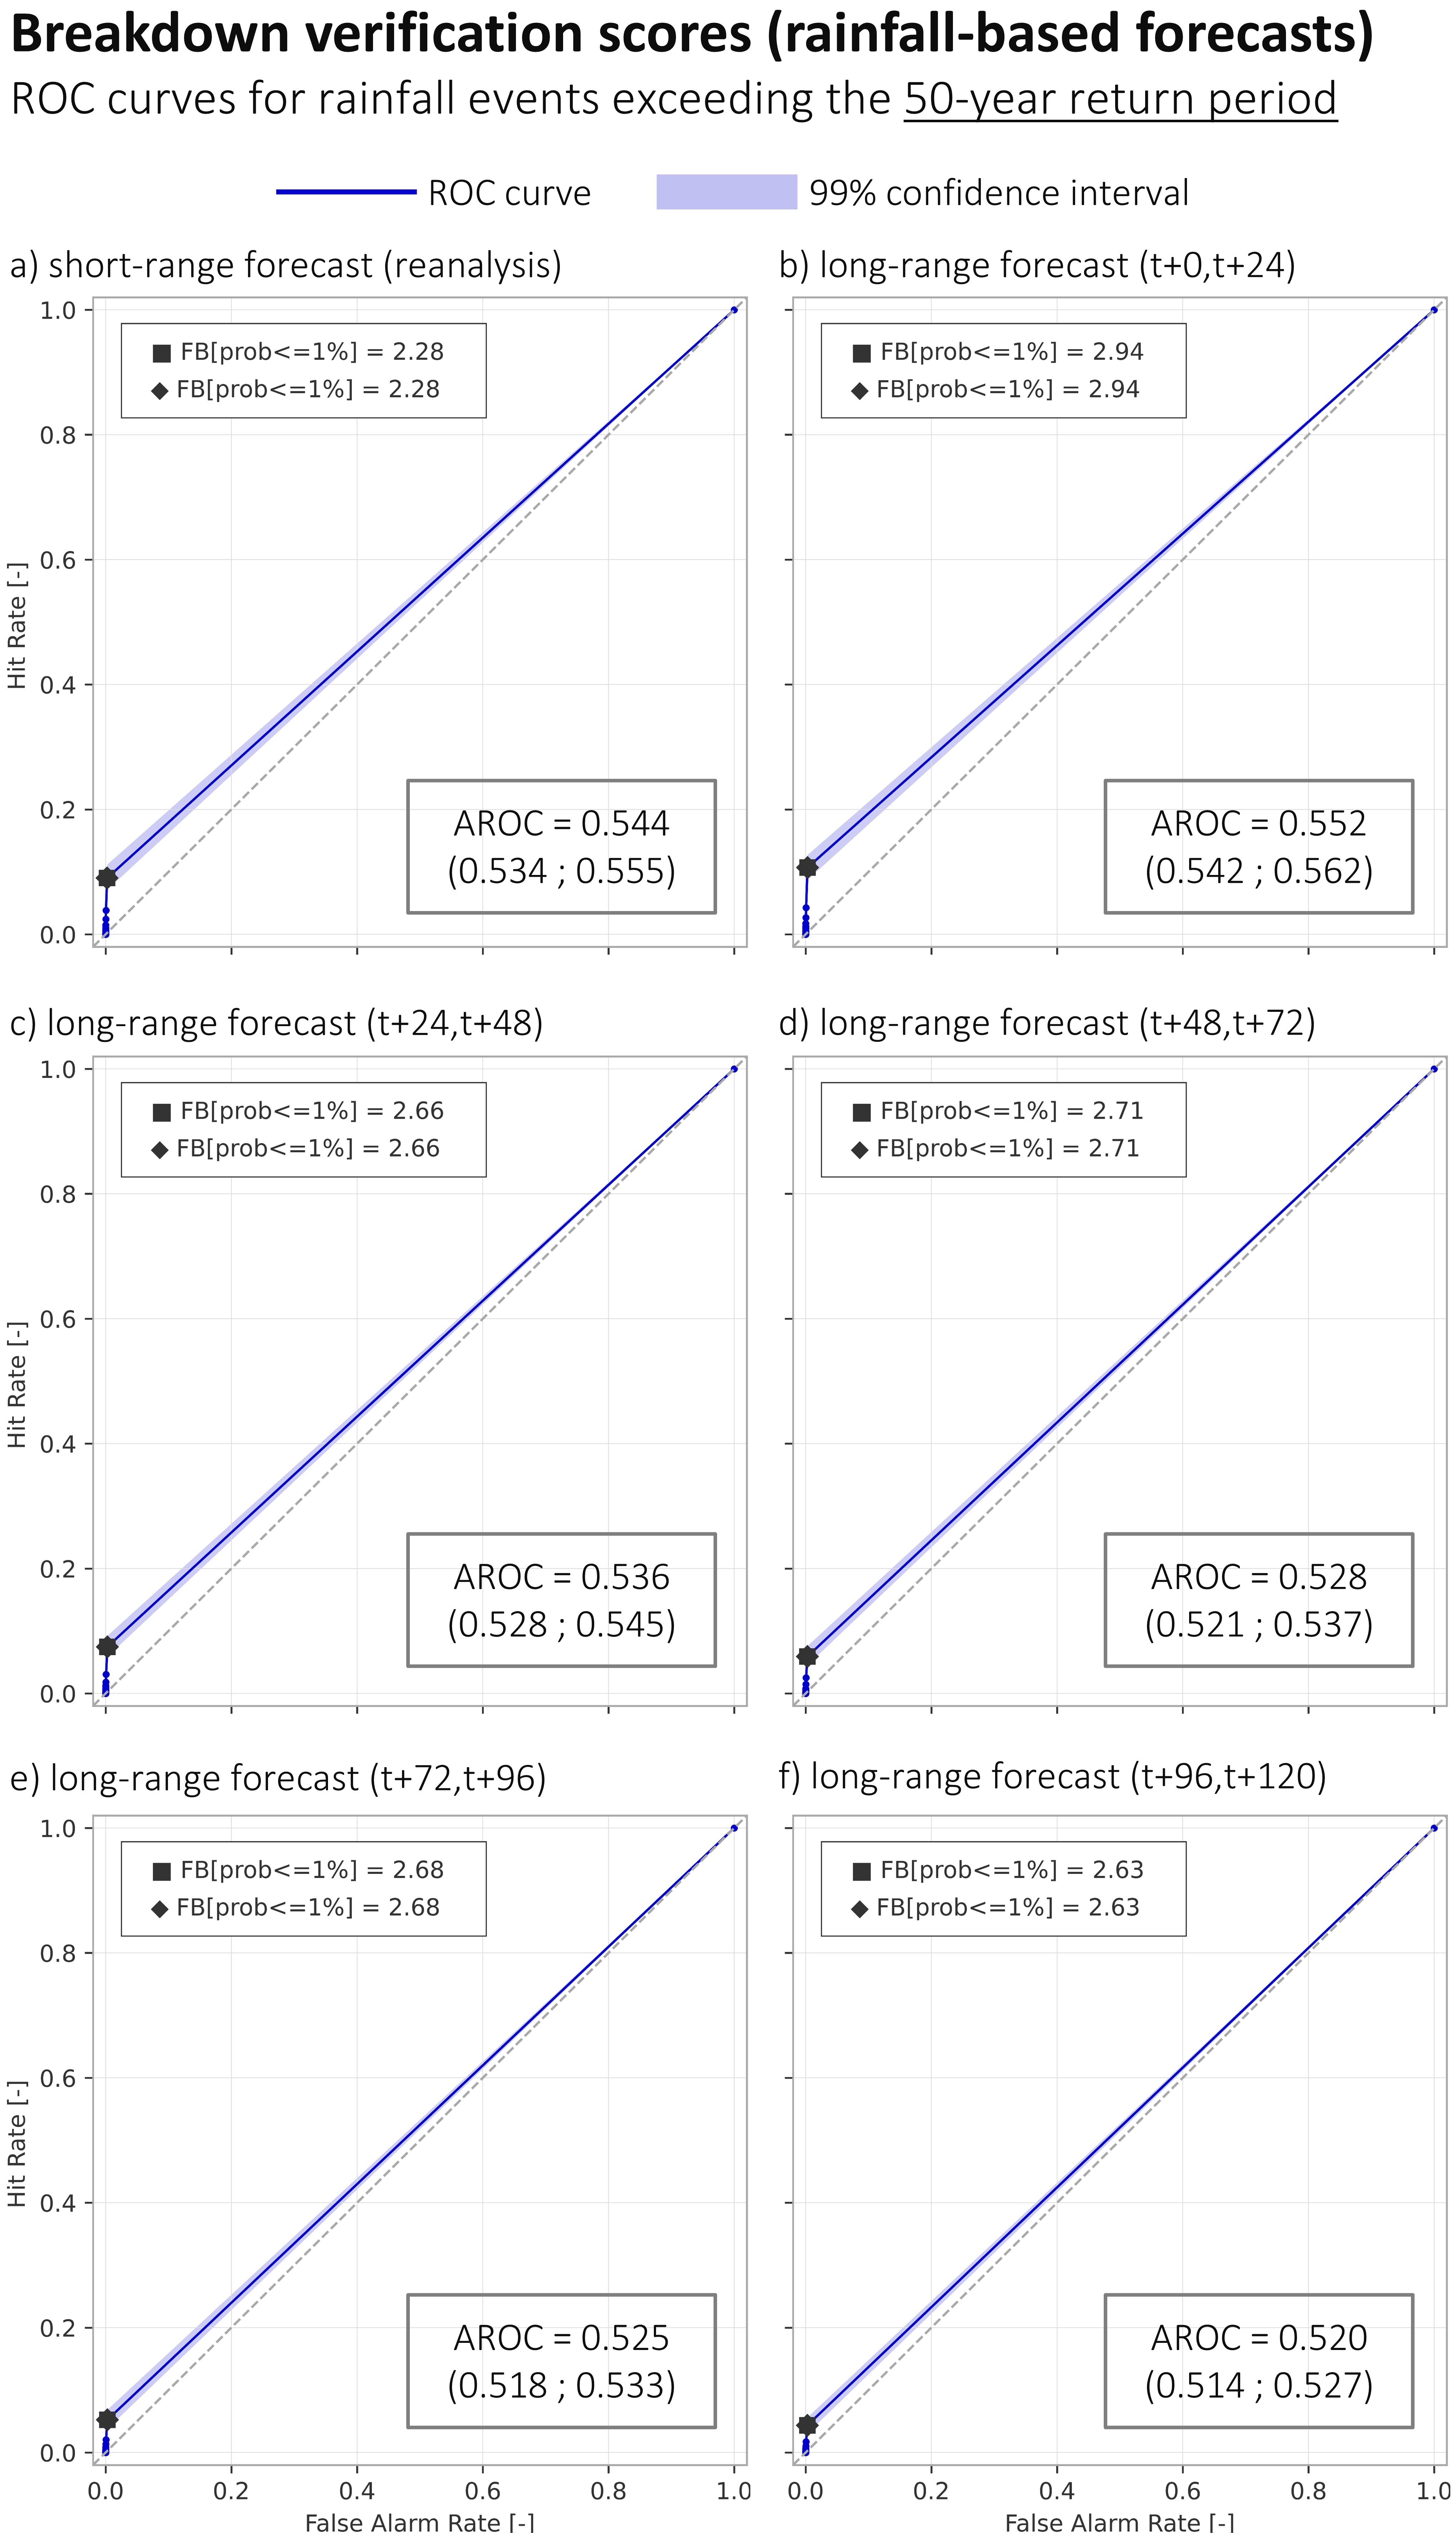
\includegraphics[width=\textwidth]{chapter_05/figures/rainfall_based_ff_verif_breakdown_scores_roc_50rp.png}
\caption{\textbf{ROC curves for tp >= 50-year return period for the rainfall-based forecasts of areas at risk of flash floods built with ERA5-ecPoint.} Similar to Figure \ref{fig:rainfall_based_ff_verif_breakdown_scores_roc_1rp}.}
\label{fig:rainfall_based_ff_verif_breakdown_scores_roc_50rp}
\end{figure}

\begin{figure}[htbp]
\centering
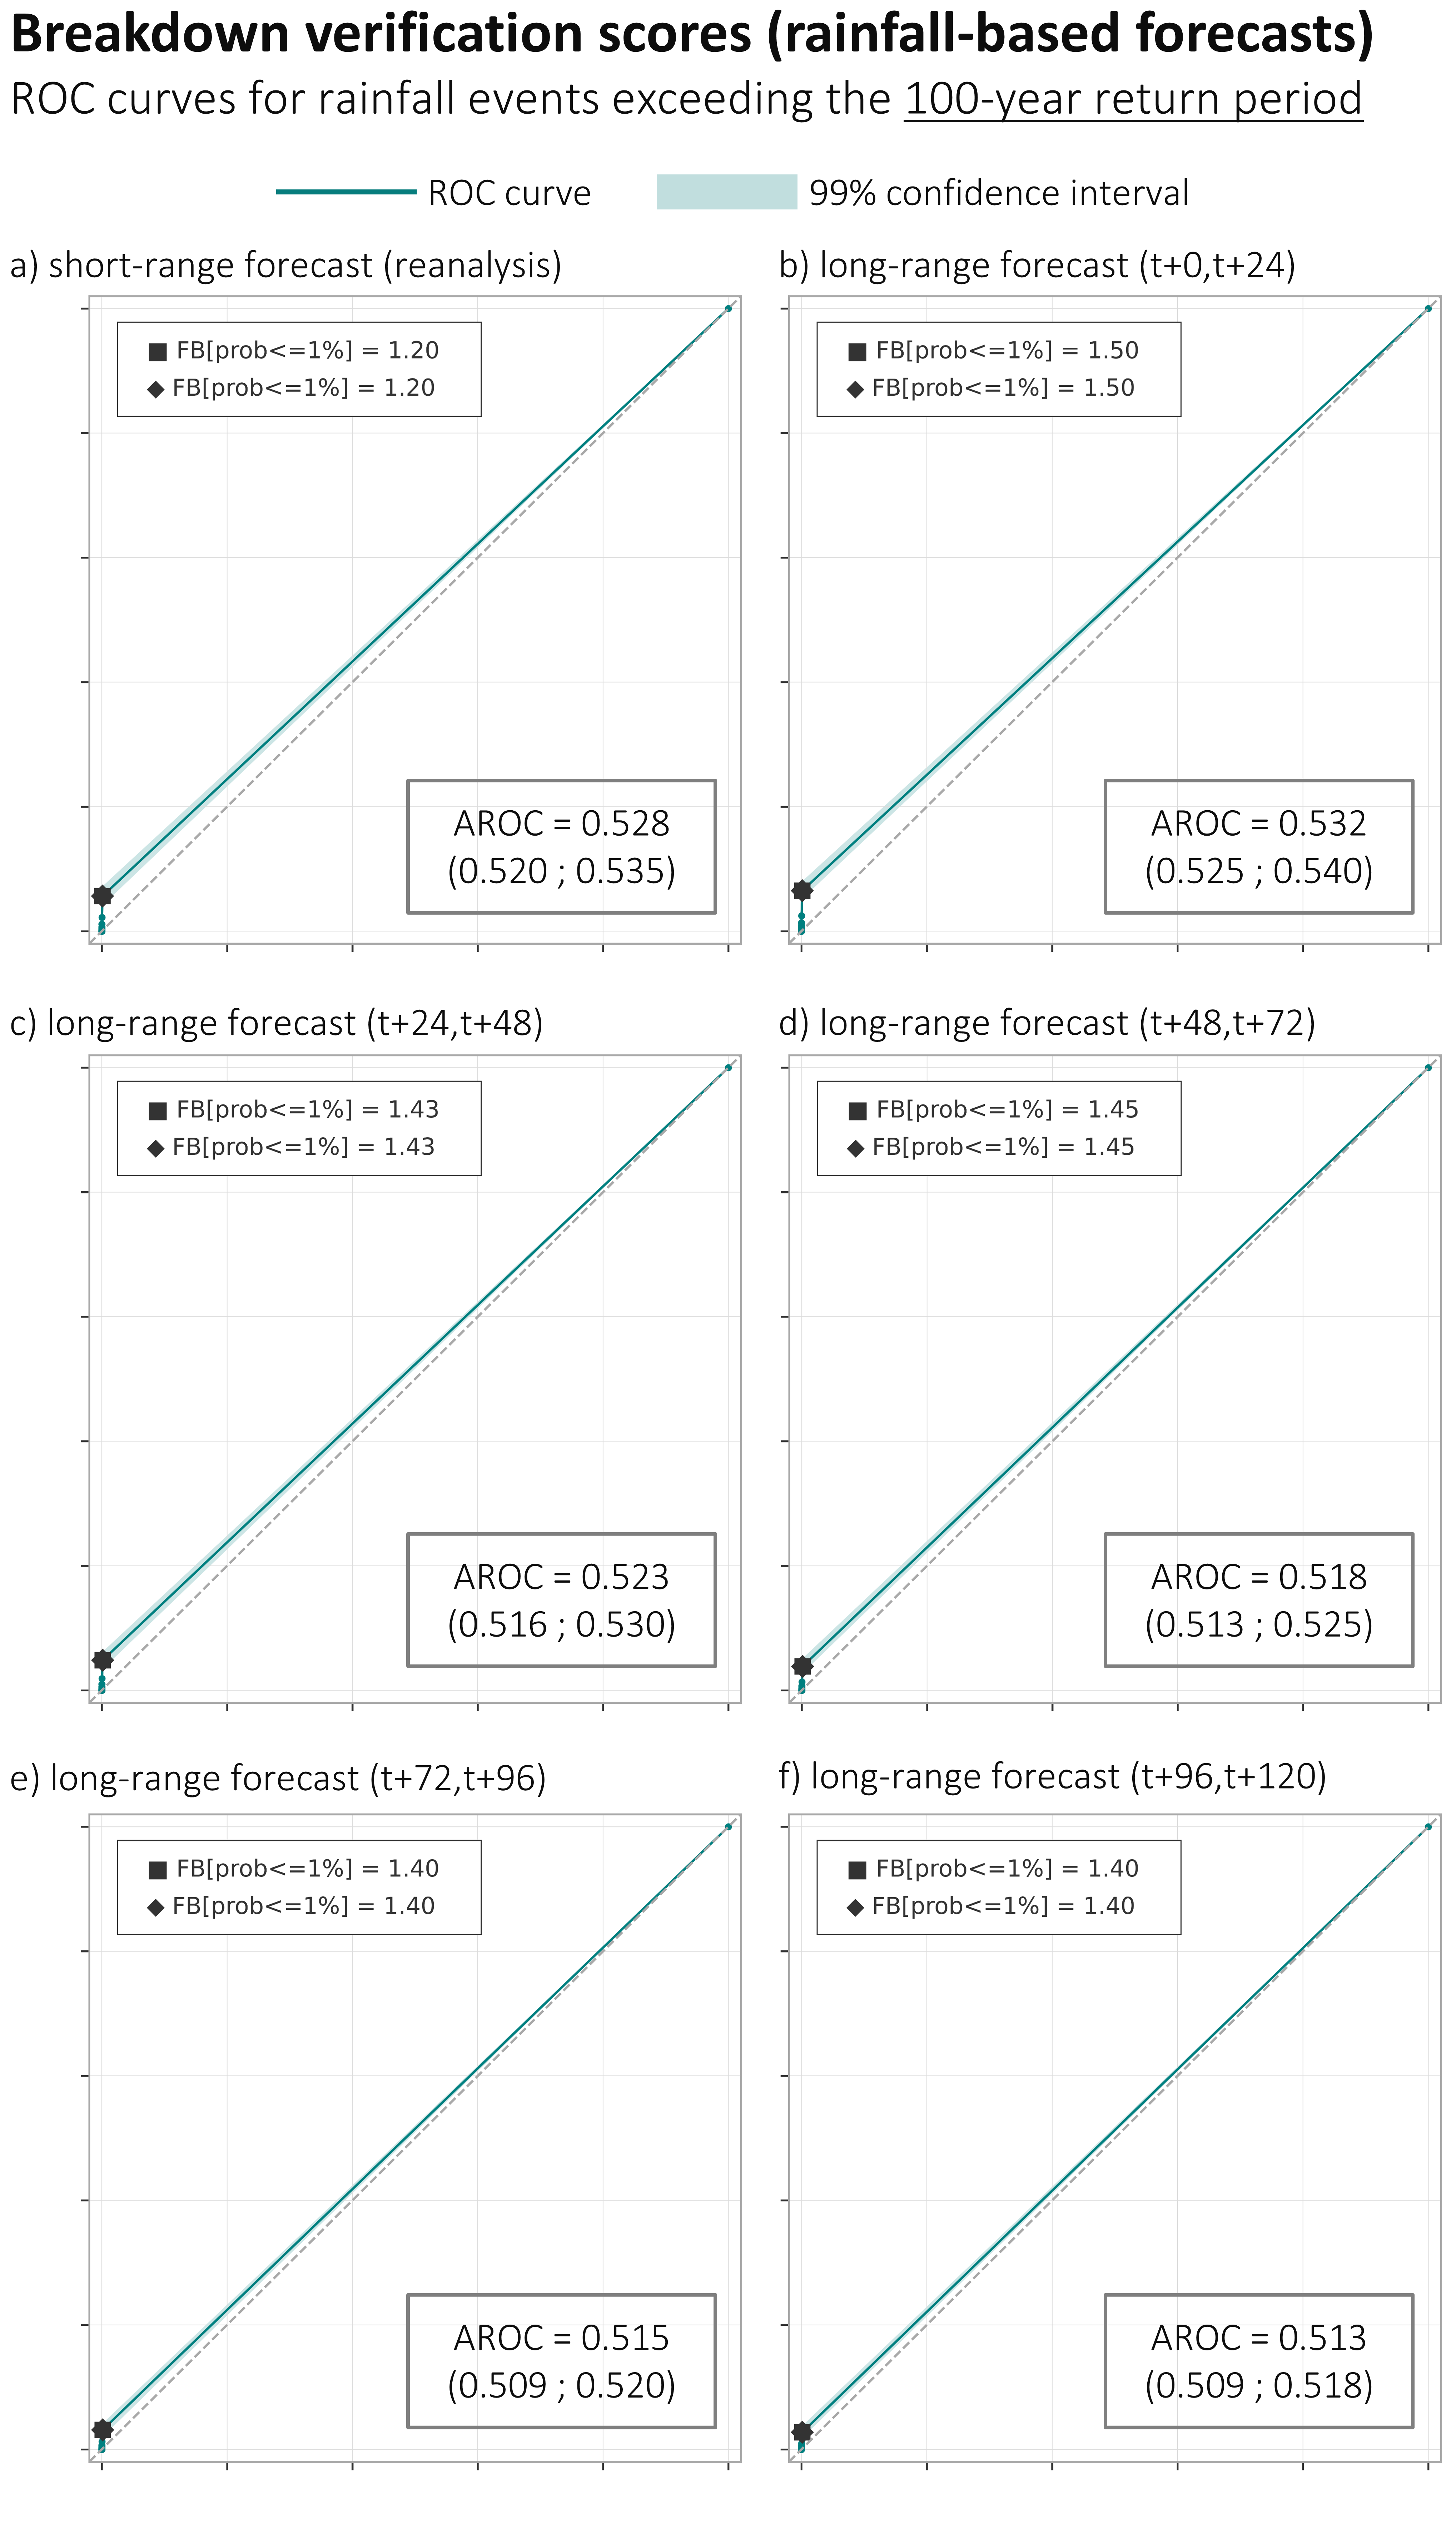
\includegraphics[width=\textwidth]{chapter_05/figures/rainfall_based_ff_verif_breakdown_scores_roc_100rp.png}
\caption{\textbf{ROC curves for tp >= 100-year return period for the rainfall-based forecasts of areas at risk of flash floods built with ERA5-ecPoint.} Similar to Figure \ref{fig:rainfall_based_ff_verif_breakdown_scores_roc_1rp}.}
\label{fig:rainfall_based_ff_verif_breakdown_scores_roc_100rp}
\end{figure}


\subsection{Reliability}

All forecasts for rainfall events exceeding the 1-year return period threshold (Figure \ref{fig:rainfall_based_ff_verif_breakdown_scores_rel_diag_1rp}) exhibit a systematic overprediction across all lead times, as shown by the reliability diagram being below the diagonal line. This indicates that when the model predicts a given probability, the observed frequency of flash flood events is consistently lower. For example, when the forecasts indicate a 50\% chance of having a flash flood event, the observed frequency ranges from \sim10\% in the short-range forecasts (Figure \ref{fig:rainfall_based_ff_verif_breakdown_scores_rel_diag_1rp}a), and between 10\% (for t+24, Figure \ref{fig:rainfall_based_ff_verif_breakdown_scores_rel_diag_1rp}b) and 2\% (t+120, Figure \ref{fig:rainfall_based_ff_verif_breakdown_scores_rel_diag_1rp}f) in the long-range forecasts. As seen in the ROC curves, the confidence intervals at 99\% are fairly narrow, suggesting that the differences between the reliability diagrams at different lead times are significant at the considered confidence level. However, the confidence levels increase with increasing forecast probabilities. As seen in the corresponding sharpness diagrams (inset boxes in all panels of Figure \ref{fig:rainfall_based_ff_verif_breakdown_scores_rel_diag_1rp}), such widening of the confidence intervals is likely due to the low number of forecasts issued with probabilities higher than ~25\% (when the total number of instances lies below 1000 samples). Such predominance of low probability forecasts suggests that the model (ERA5-ecPoint) rarely expresses high confidence in extreme event occurrence. A notable characteristic of all the reliability diagrams in the Figure \ref{fig:rainfall_based_ff_verif_breakdown_scores_rel_diag_1rp} is the sharp increase in observed frequency for the highest probability bins (i.e. 80\% to 100\%). This steep rise suggests that when the model does issue high probability forecasts, these correspond to genuinely extreme events, though such forecasts remain infrequent.

\begin{figure}[htbp]
\centering
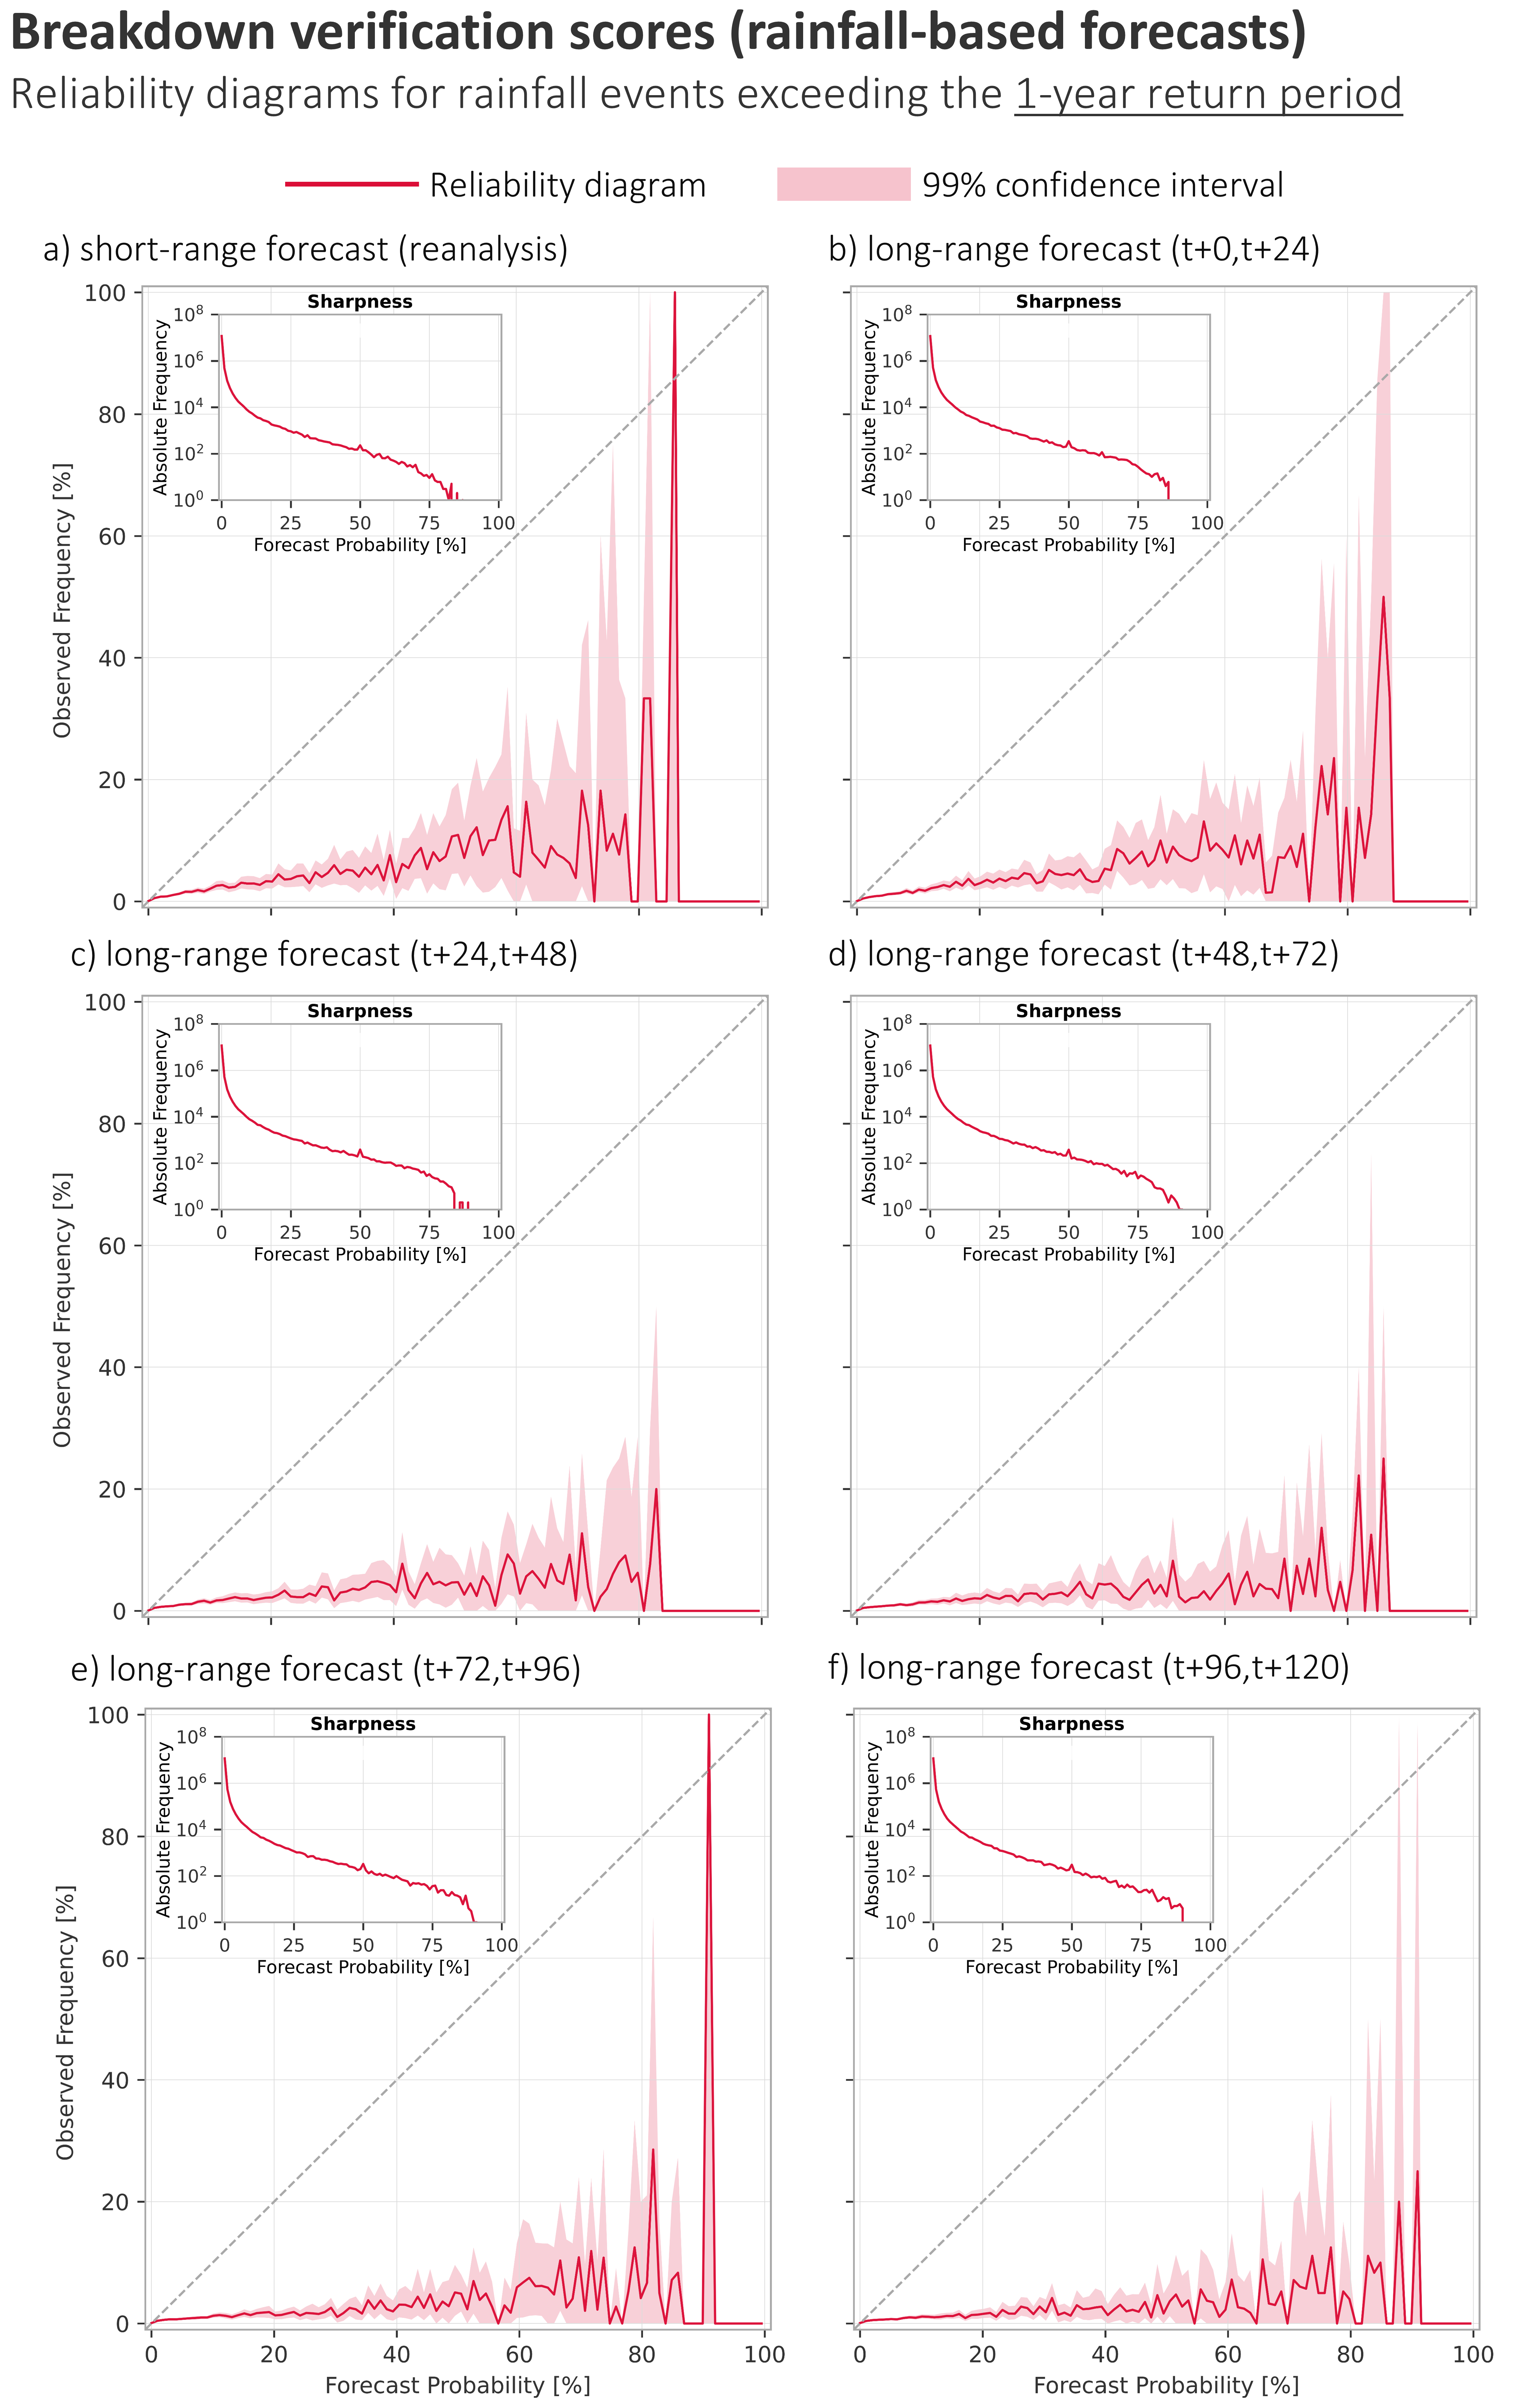
\includegraphics[width=\textwidth]{rainfall_based_ff_verif_breakdown_scores_rel_diag_1rp.png}
\caption{\textbf{Reliability diagrams for tp >= 1-year return period for the rainfall-based forecasts of areas at risk of flash floods built with ERA5-ecPoint.} Panel (a) shows the reliability diagram (blue solid line) for the short-range predictions together with the confidence intervals (blue shaded area) at 99\% confidence level. Panels (b) to (f) refer to the long-range forecasts for accumulation periods ending in t+24, t+48, t+72, t+96, and t+120, respectively. The inset boxes show the corresponding sharpness diagrams.}
\label{fig:rainfall_based_ff_verif_breakdown_scores_rel_diag_1rp}
\end{figure}

The temporal evolution from Figure \ref{fig:rainfall_based_ff_verif_breakdown_scores_rel_diag_1rp}a to f reveals subtle changes in the forecasts' reliability characteristics with increasing lead time. Whilst the general pattern of overprediction persists, from day 2 forecasts (t+48) results more squashed into a flat line over very small observed frequencies, indicating that even though the model issues forecasts with high probabilities of exceeding the 1-year return period at longer lead times with a similar frequency of the short-range forecasts and the day 1 (t+24) long-range forecast, such forecasts do not necessarily correspond to an observed flash flood event.

The reliability diagrams get closer to the diagonal line (indicating perfect bias) as we increase the rainfall threshold to identify the flash flood events. Perfect reliability is observed for rainfall events exceeding the 10-, 20-year, and 50-year return period with probabilities below 5\% at day 1 forecast (t+24) for the 10-, 20-year return period, and 10\% for the 50-year return period.

\begin{figure}[htbp]
\centering
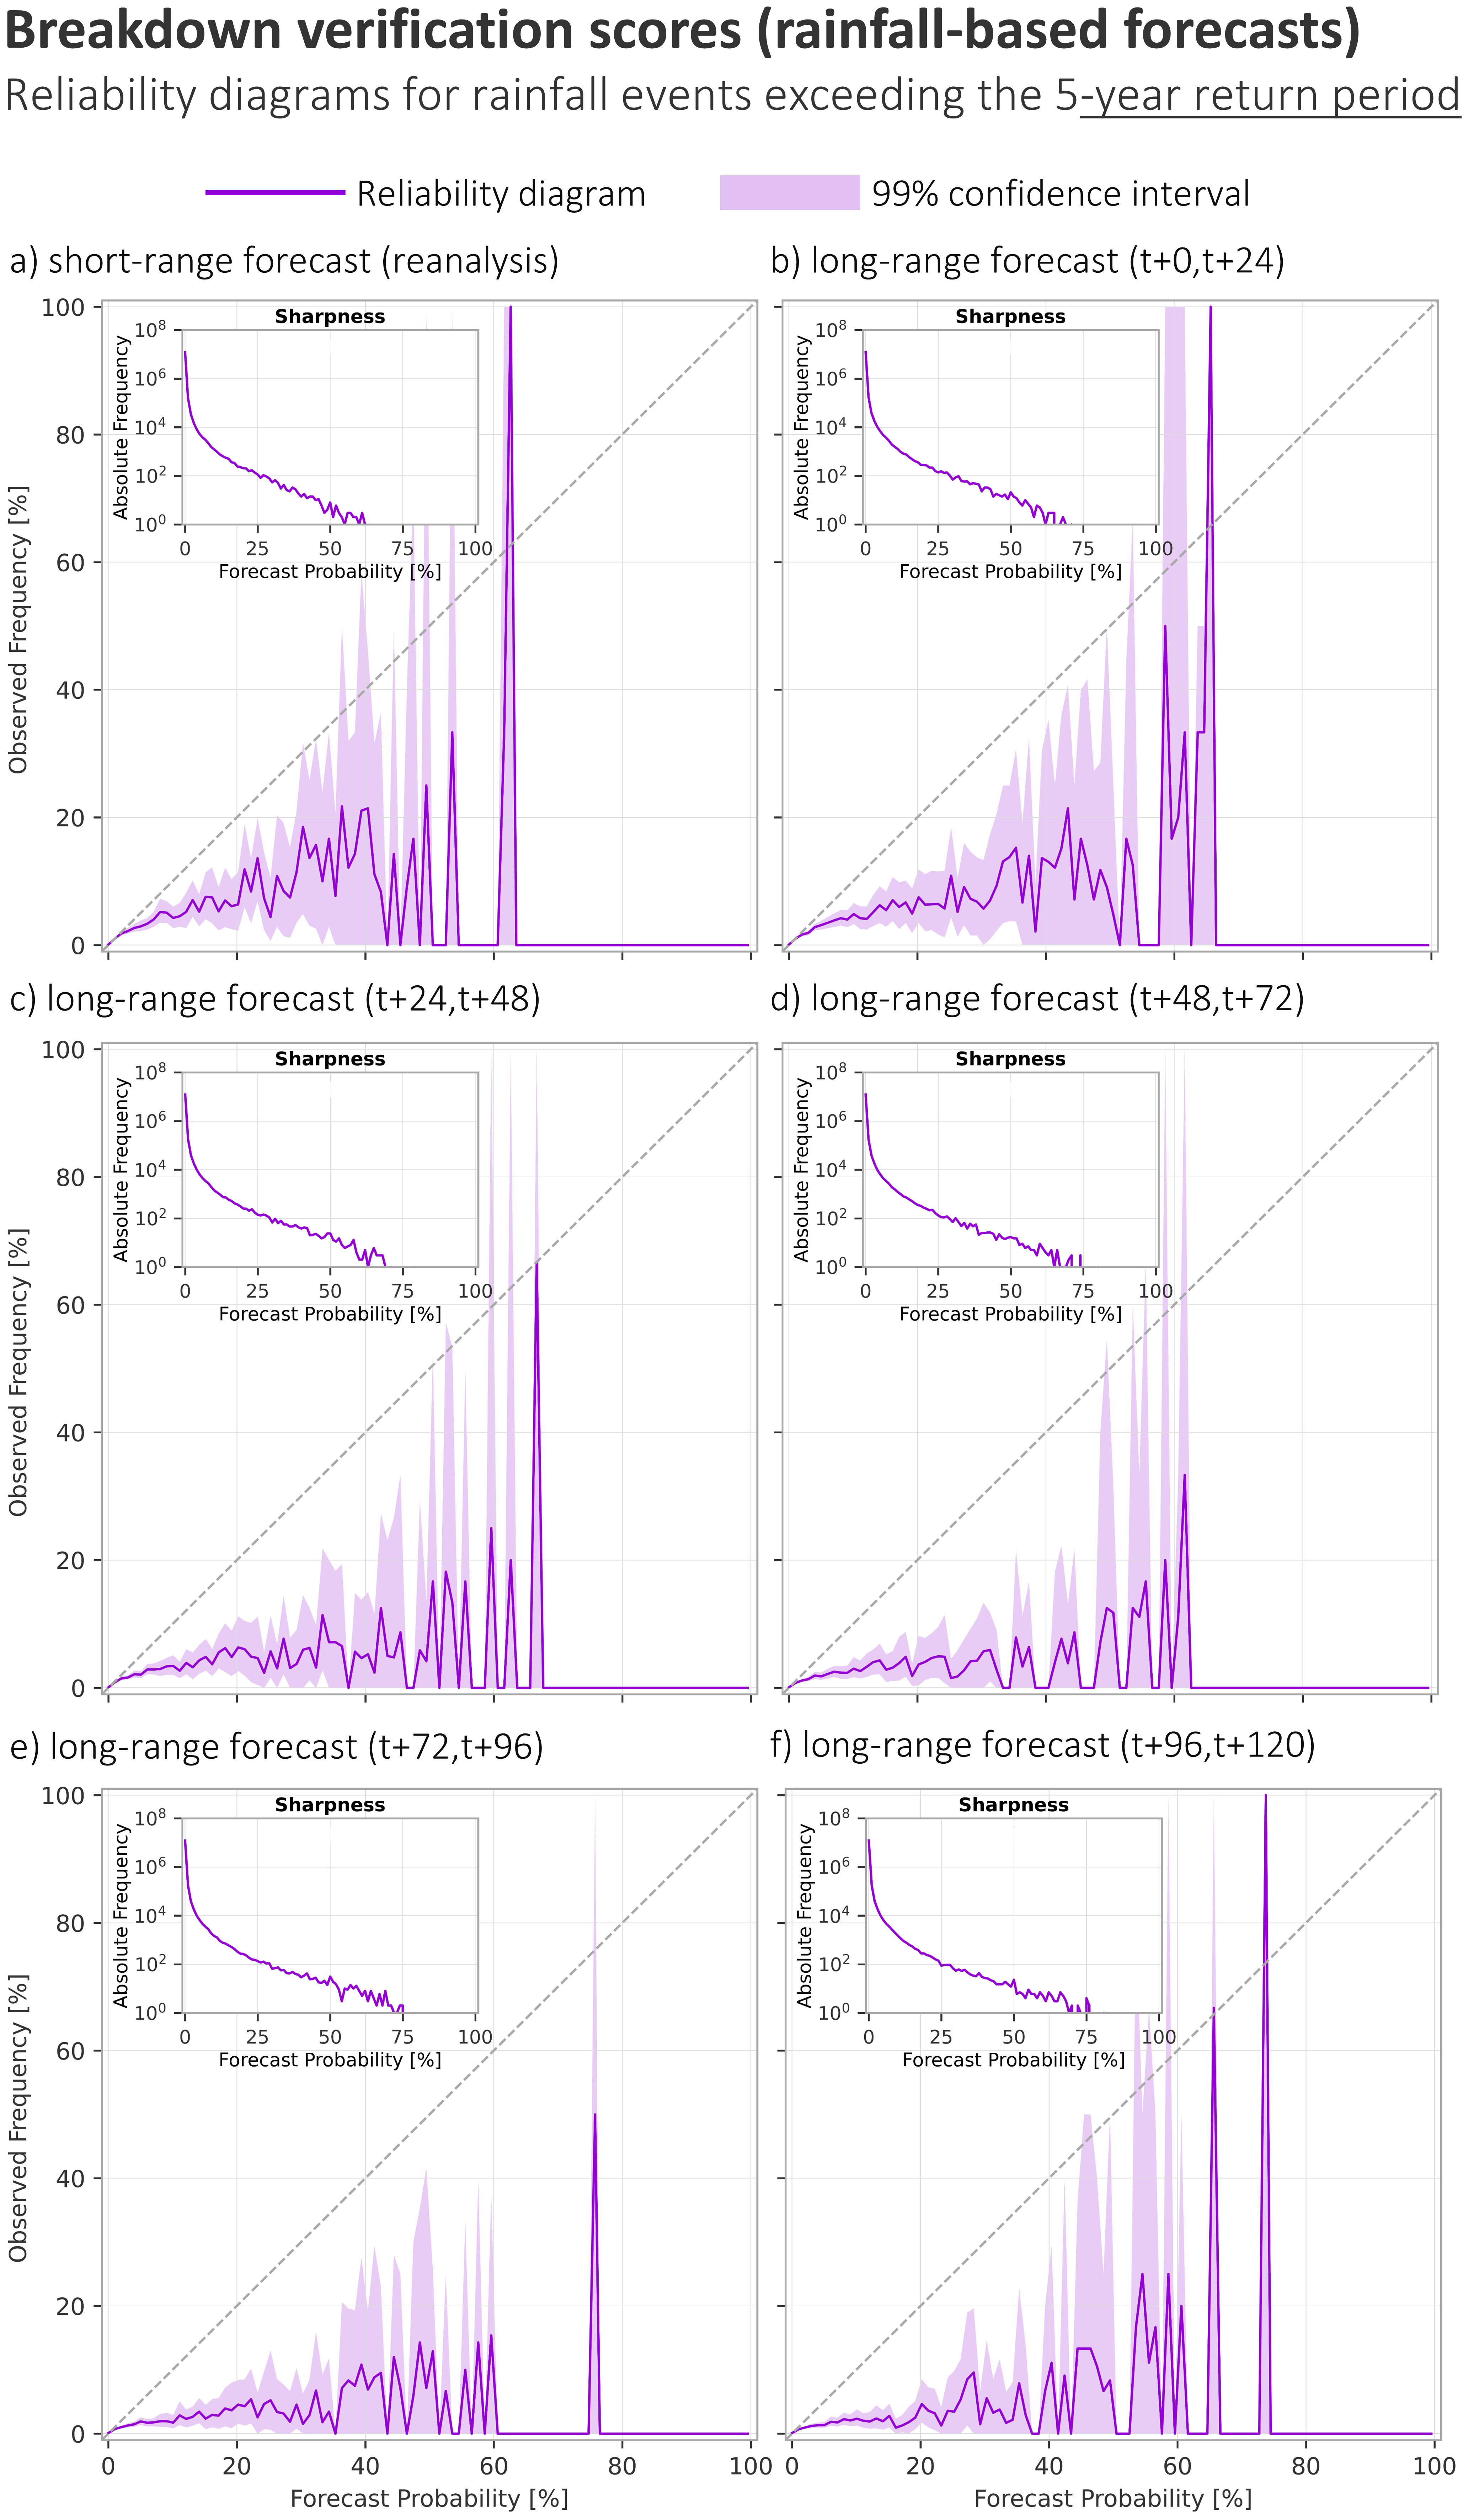
\includegraphics[width=\textwidth]{rainfall_based_ff_verif_breakdown_scores_rel_diag_5rp.png}
\caption{\textbf{Reliability diagrams for tp >= 5-year return period for the rainfall-based forecasts of areas at risk of flash floods built with ERA5-ecPoint.} Similar to Figure \ref{fig:rainfall_based_ff_verif_breakdown_scores_rel_diag_1rp}.}
\label{fig:rainfall_based_ff_verif_breakdown_scores_rel_diag_5rp}
\end{figure}

\begin{figure}[htbp]
\centering
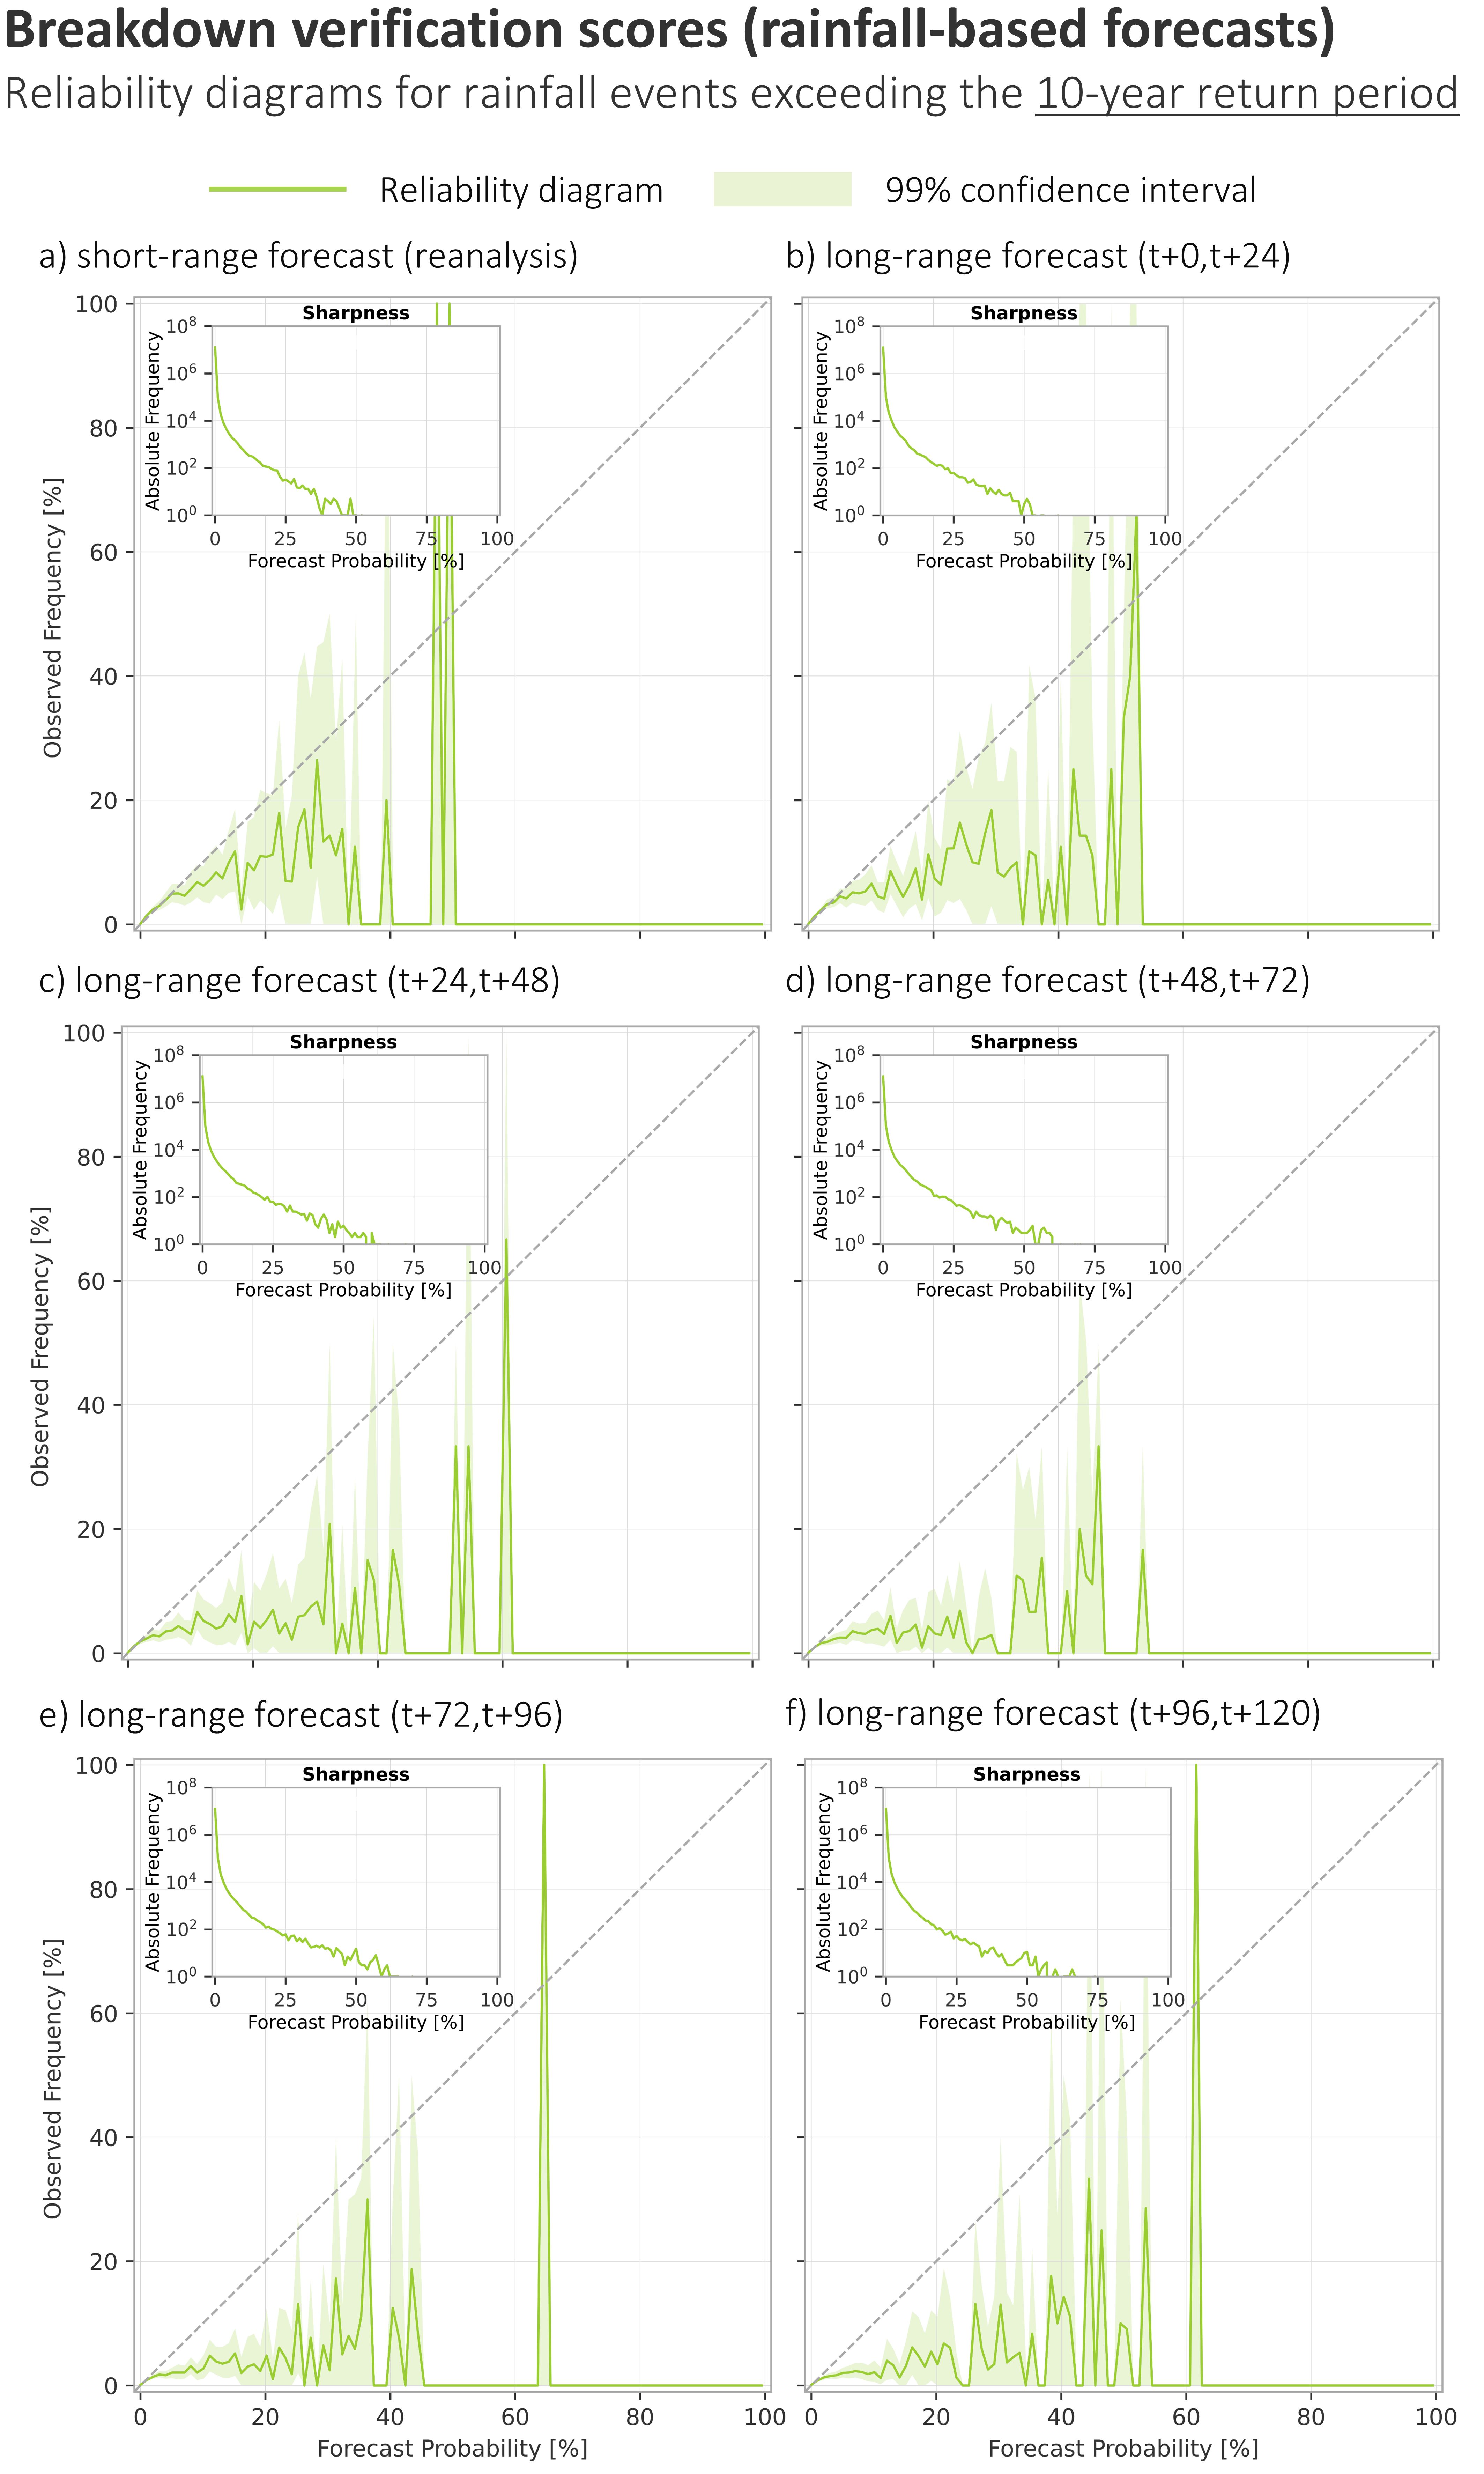
\includegraphics[width=\textwidth]{rainfall_based_ff_verif_breakdown_scores_rel_diag_10rp.png}
\caption{\textbf{Reliability diagrams for tp >= 5-year return period for the rainfall-based forecasts of areas at risk of flash floods built with ERA5-ecPoint.} Similar to Figure \ref{fig:rainfall_based_ff_verif_breakdown_scores_rel_diag_1rp}.}
\label{fig:rainfall_based_ff_verif_breakdown_scores_rel_diag_10rp}
\end{figure}

\begin{figure}[htbp]
\centering
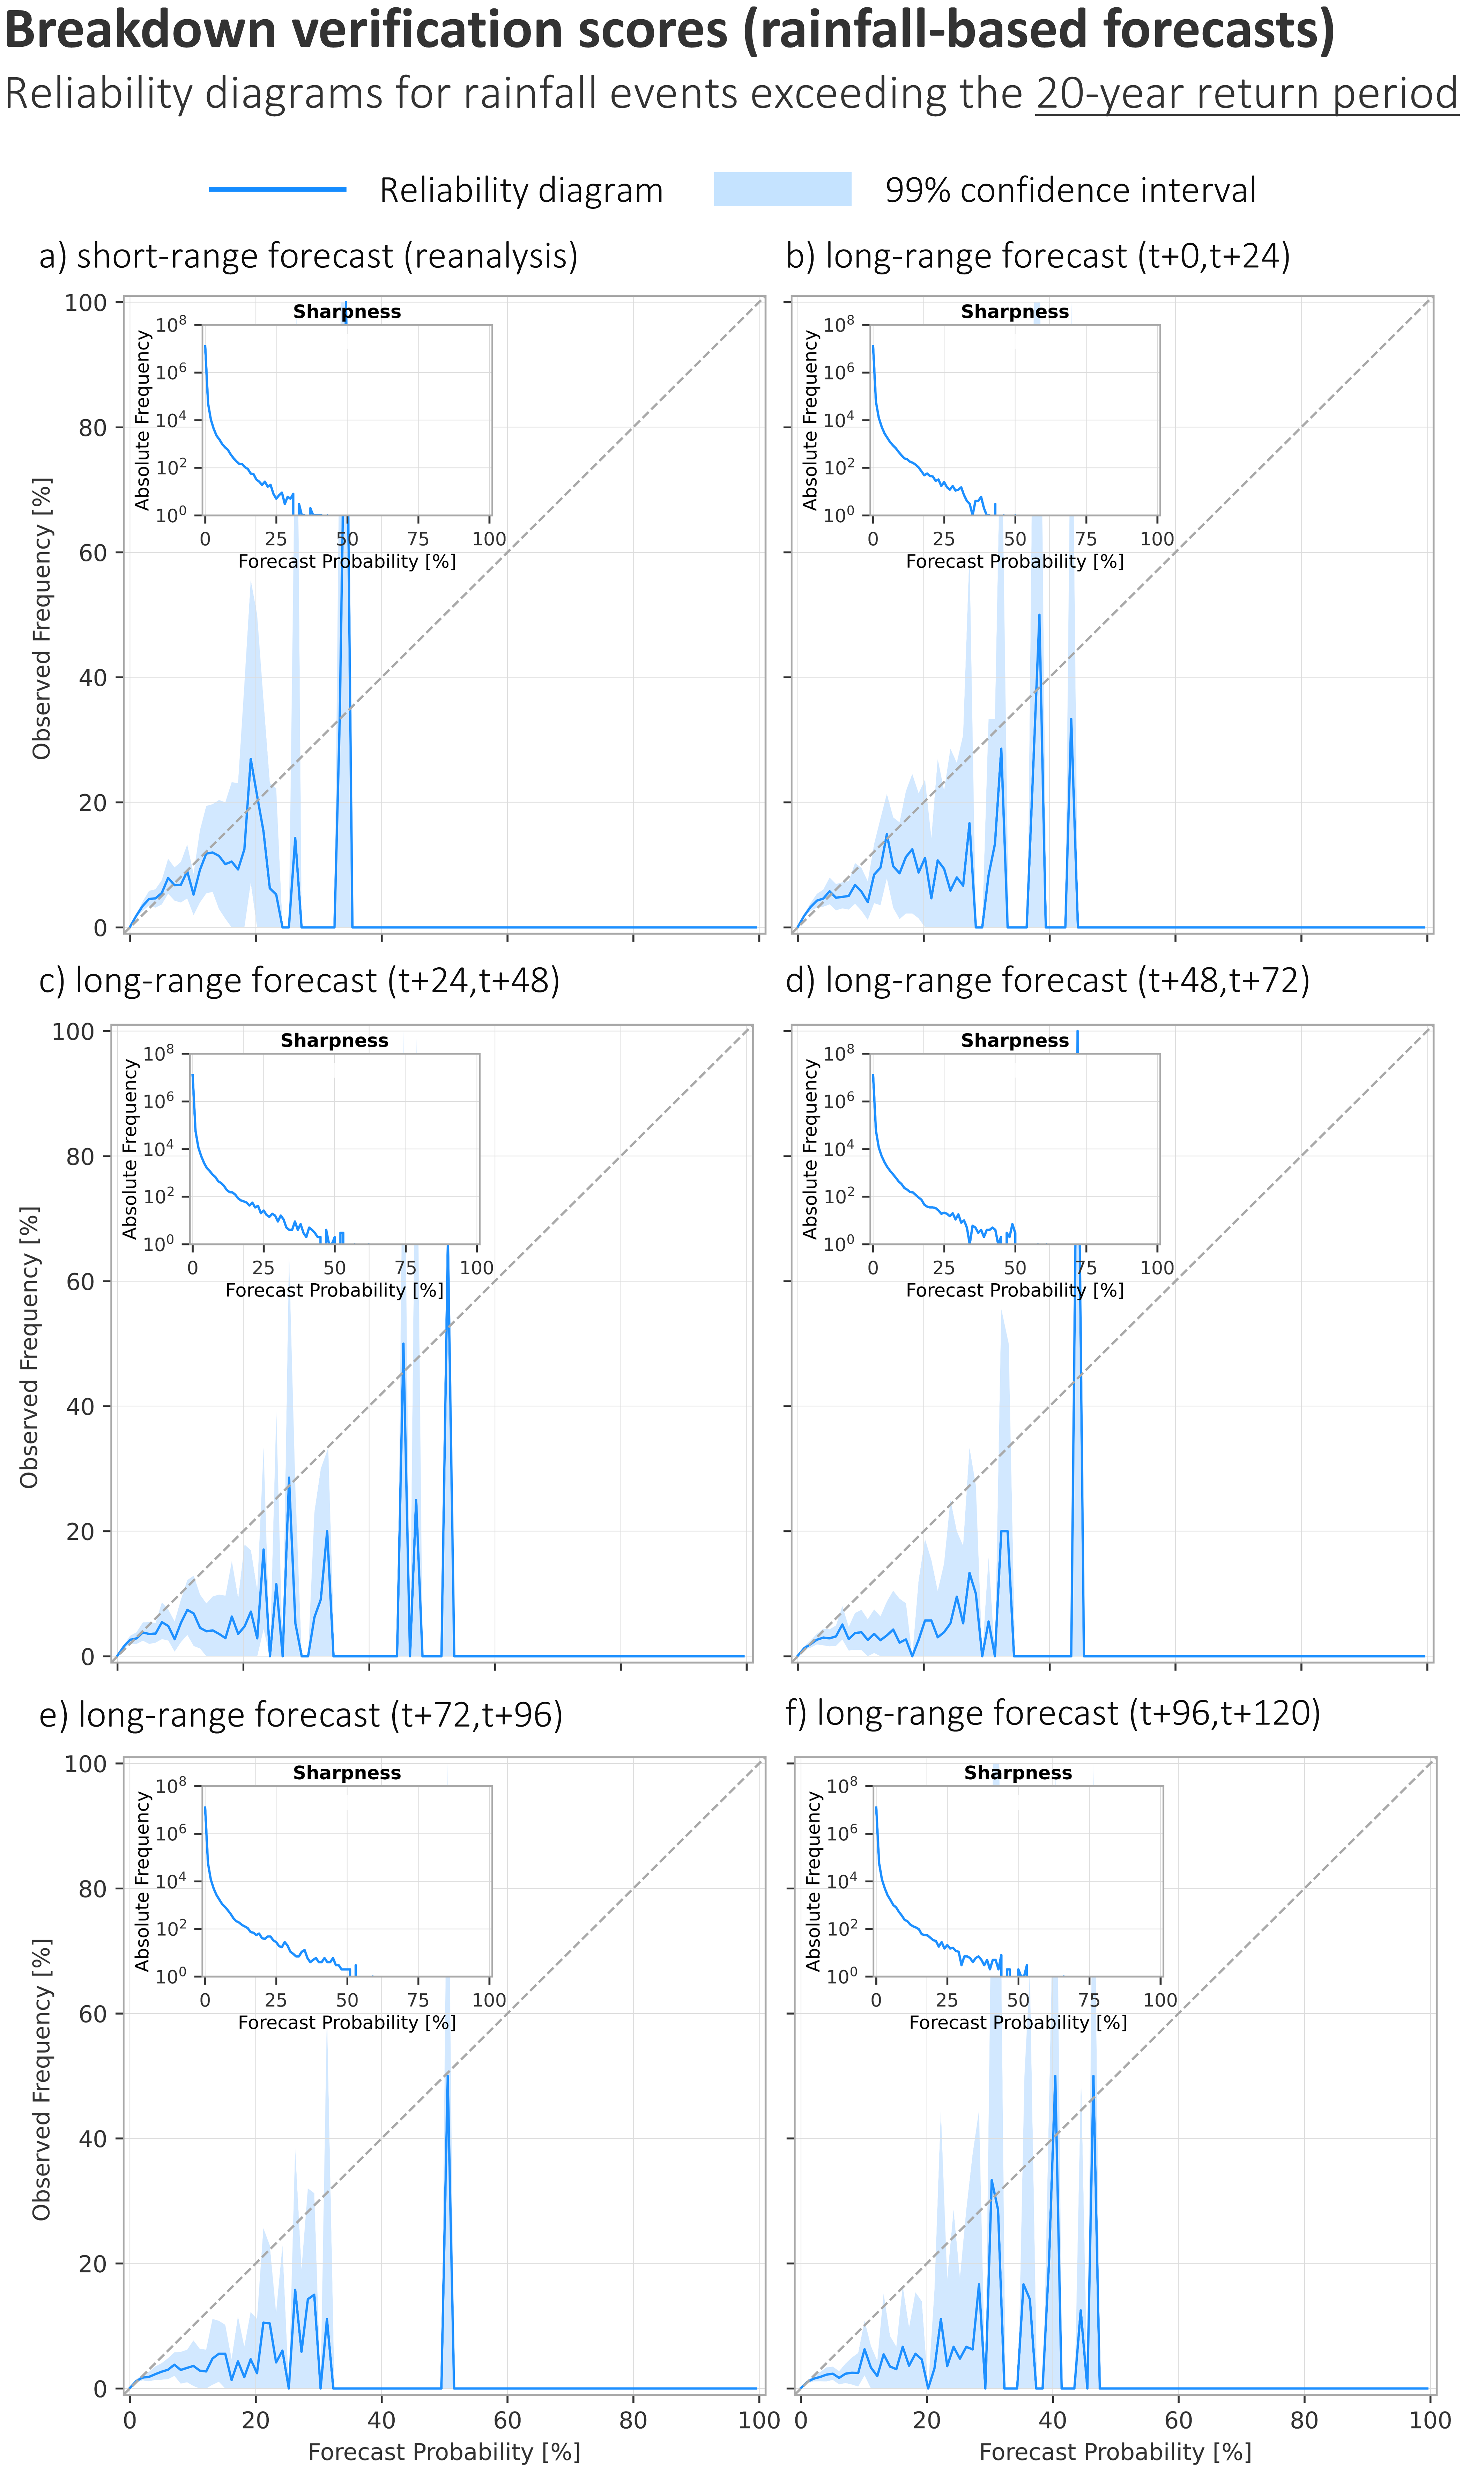
\includegraphics[width=\textwidth]{rainfall_based_ff_verif_breakdown_scores_rel_diag_20rp.png}
\caption{\textbf{Reliability diagrams for tp >= 5-year return period for the rainfall-based forecasts of areas at risk of flash floods built with ERA5-ecPoint.} Similar to Figure \ref{fig:rainfall_based_ff_verif_breakdown_scores_rel_diag_1rp}.}
\label{fig:rainfall_based_ff_verif_breakdown_scores_rel_diag_20rp}
\end{figure}

\begin{figure}[htbp]
\centering
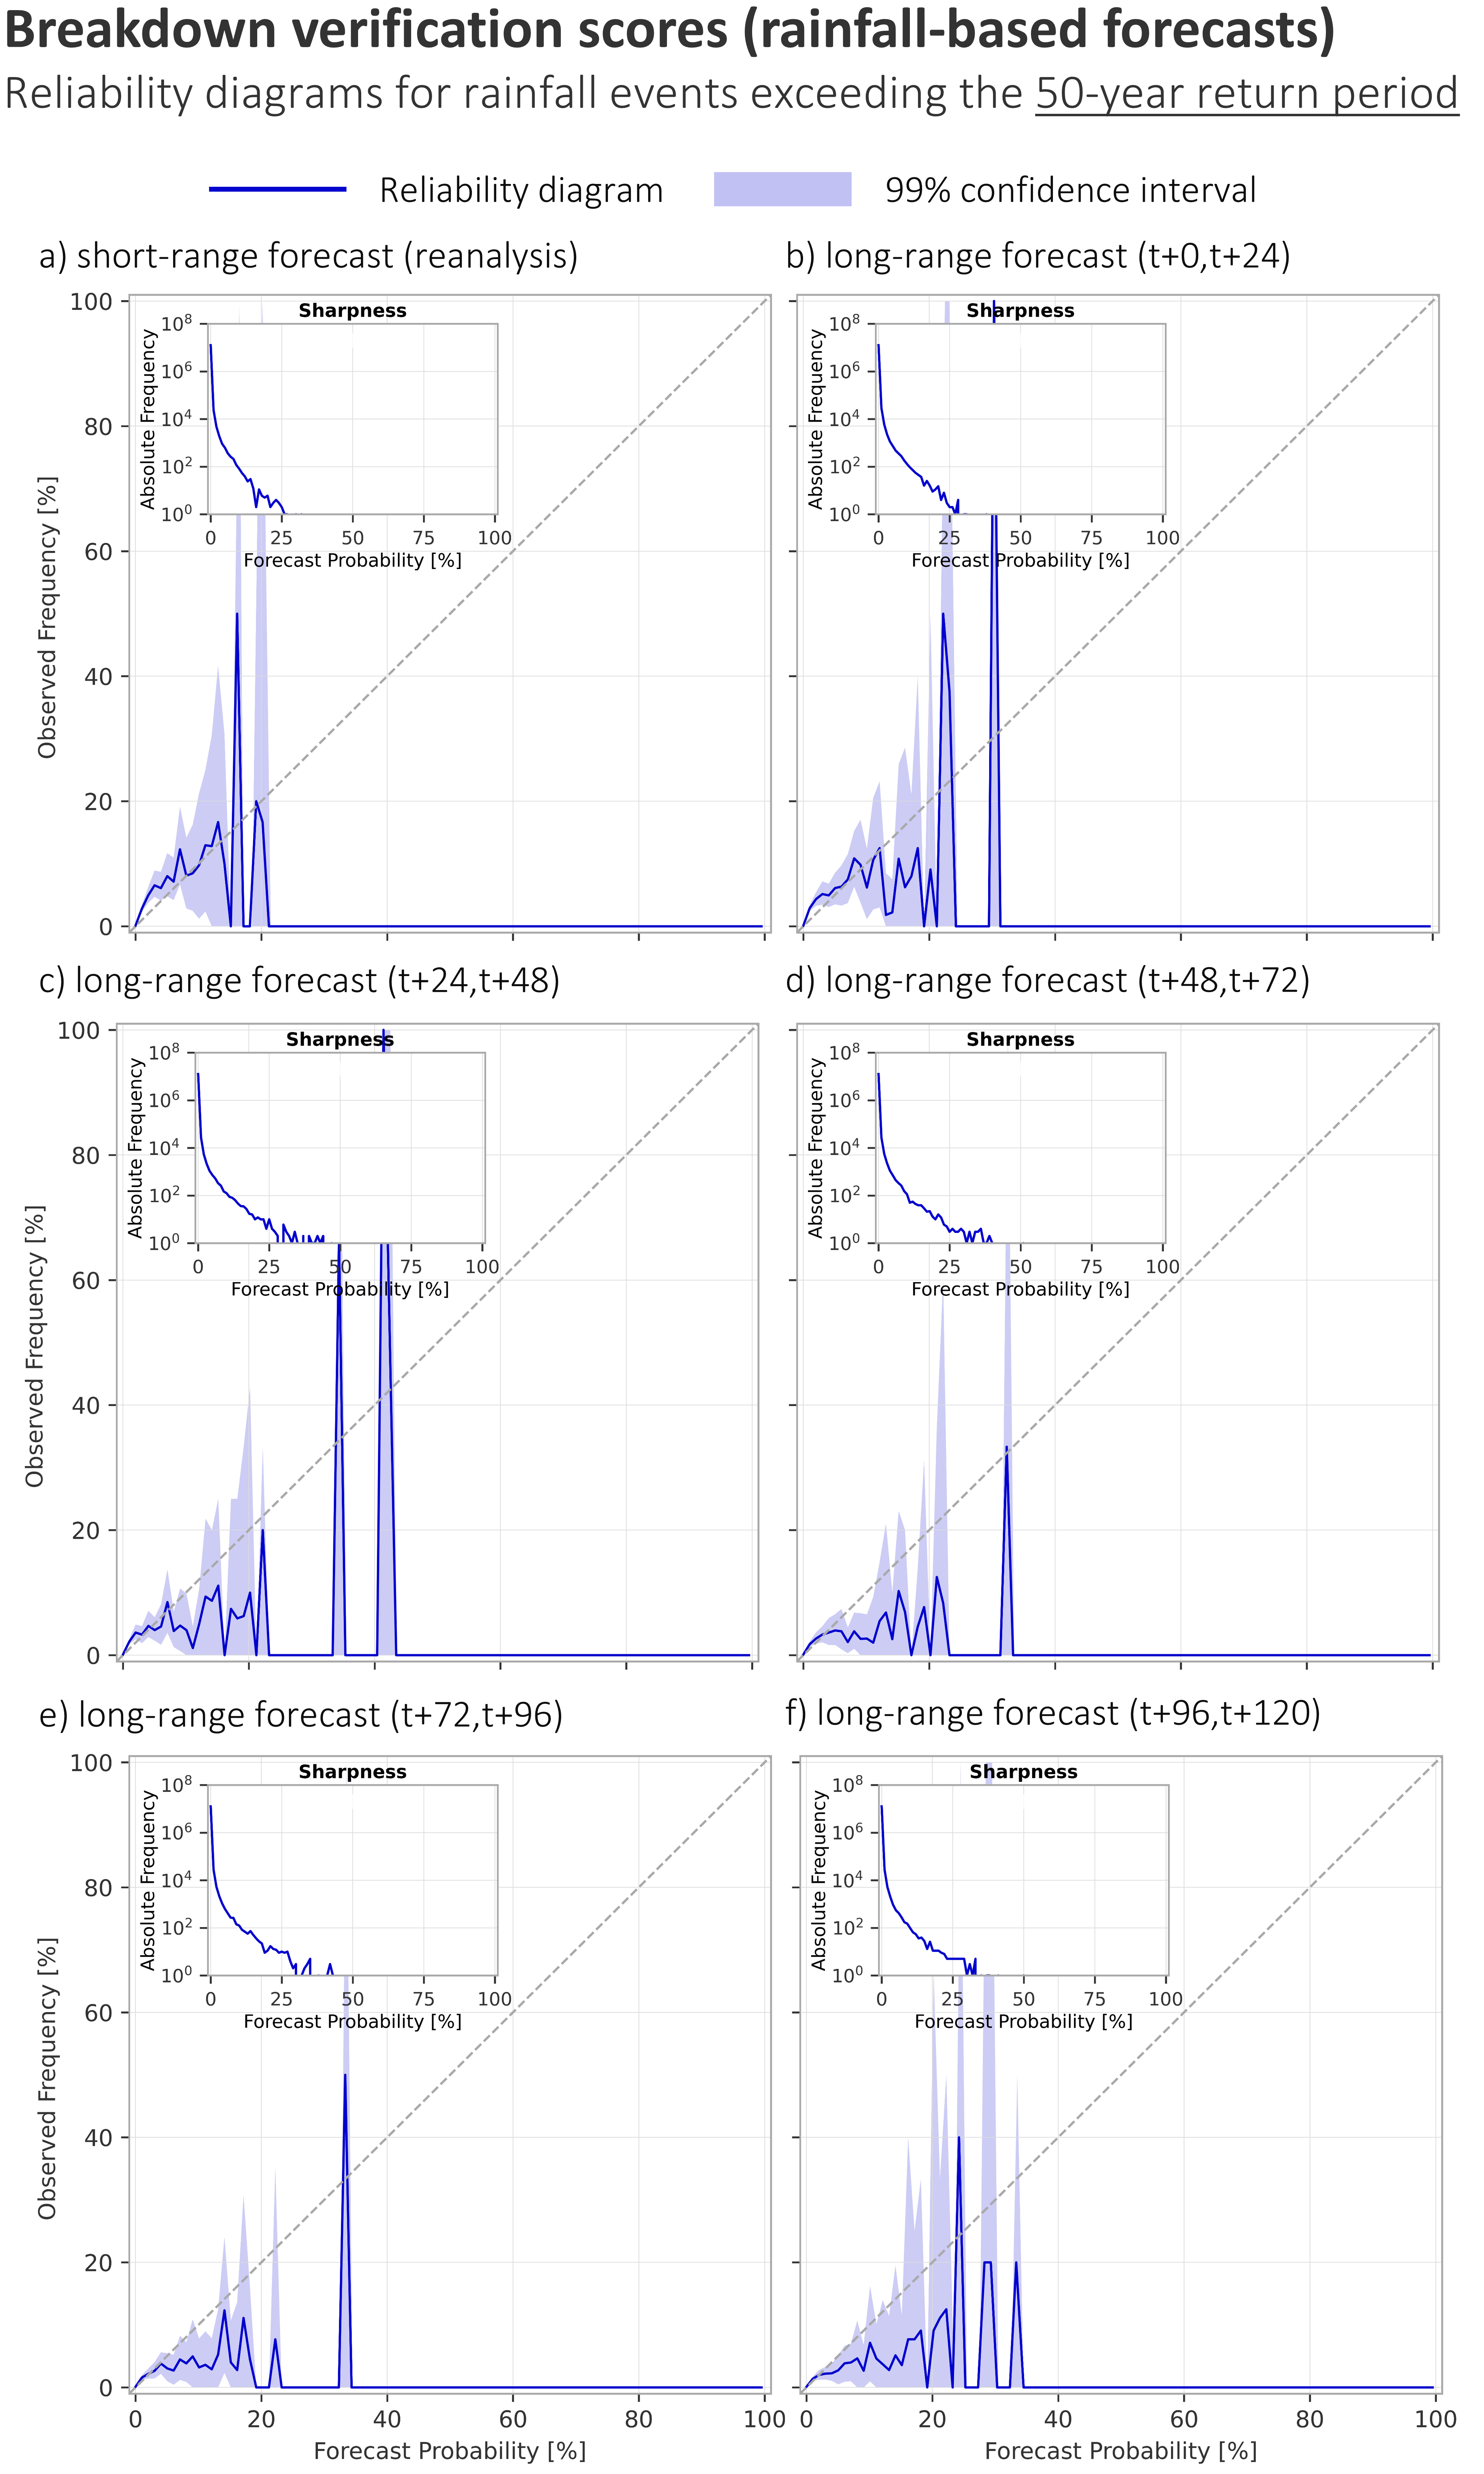
\includegraphics[width=\textwidth]{rainfall_based_ff_verif_breakdown_scores_rel_diag_50rp.png}
\caption{\textbf{Reliability diagrams for tp >= 5-year return period for the rainfall-based forecasts of areas at risk of flash floods built with ERA5-ecPoint.} Similar to Figure \ref{fig:rainfall_based_ff_verif_breakdown_scores_rel_diag_1rp}.}
\label{fig:rainfall_based_ff_verif_breakdown_scores_rel_diag_50rp}
\end{figure}

\begin{figure}[htbp]
\centering
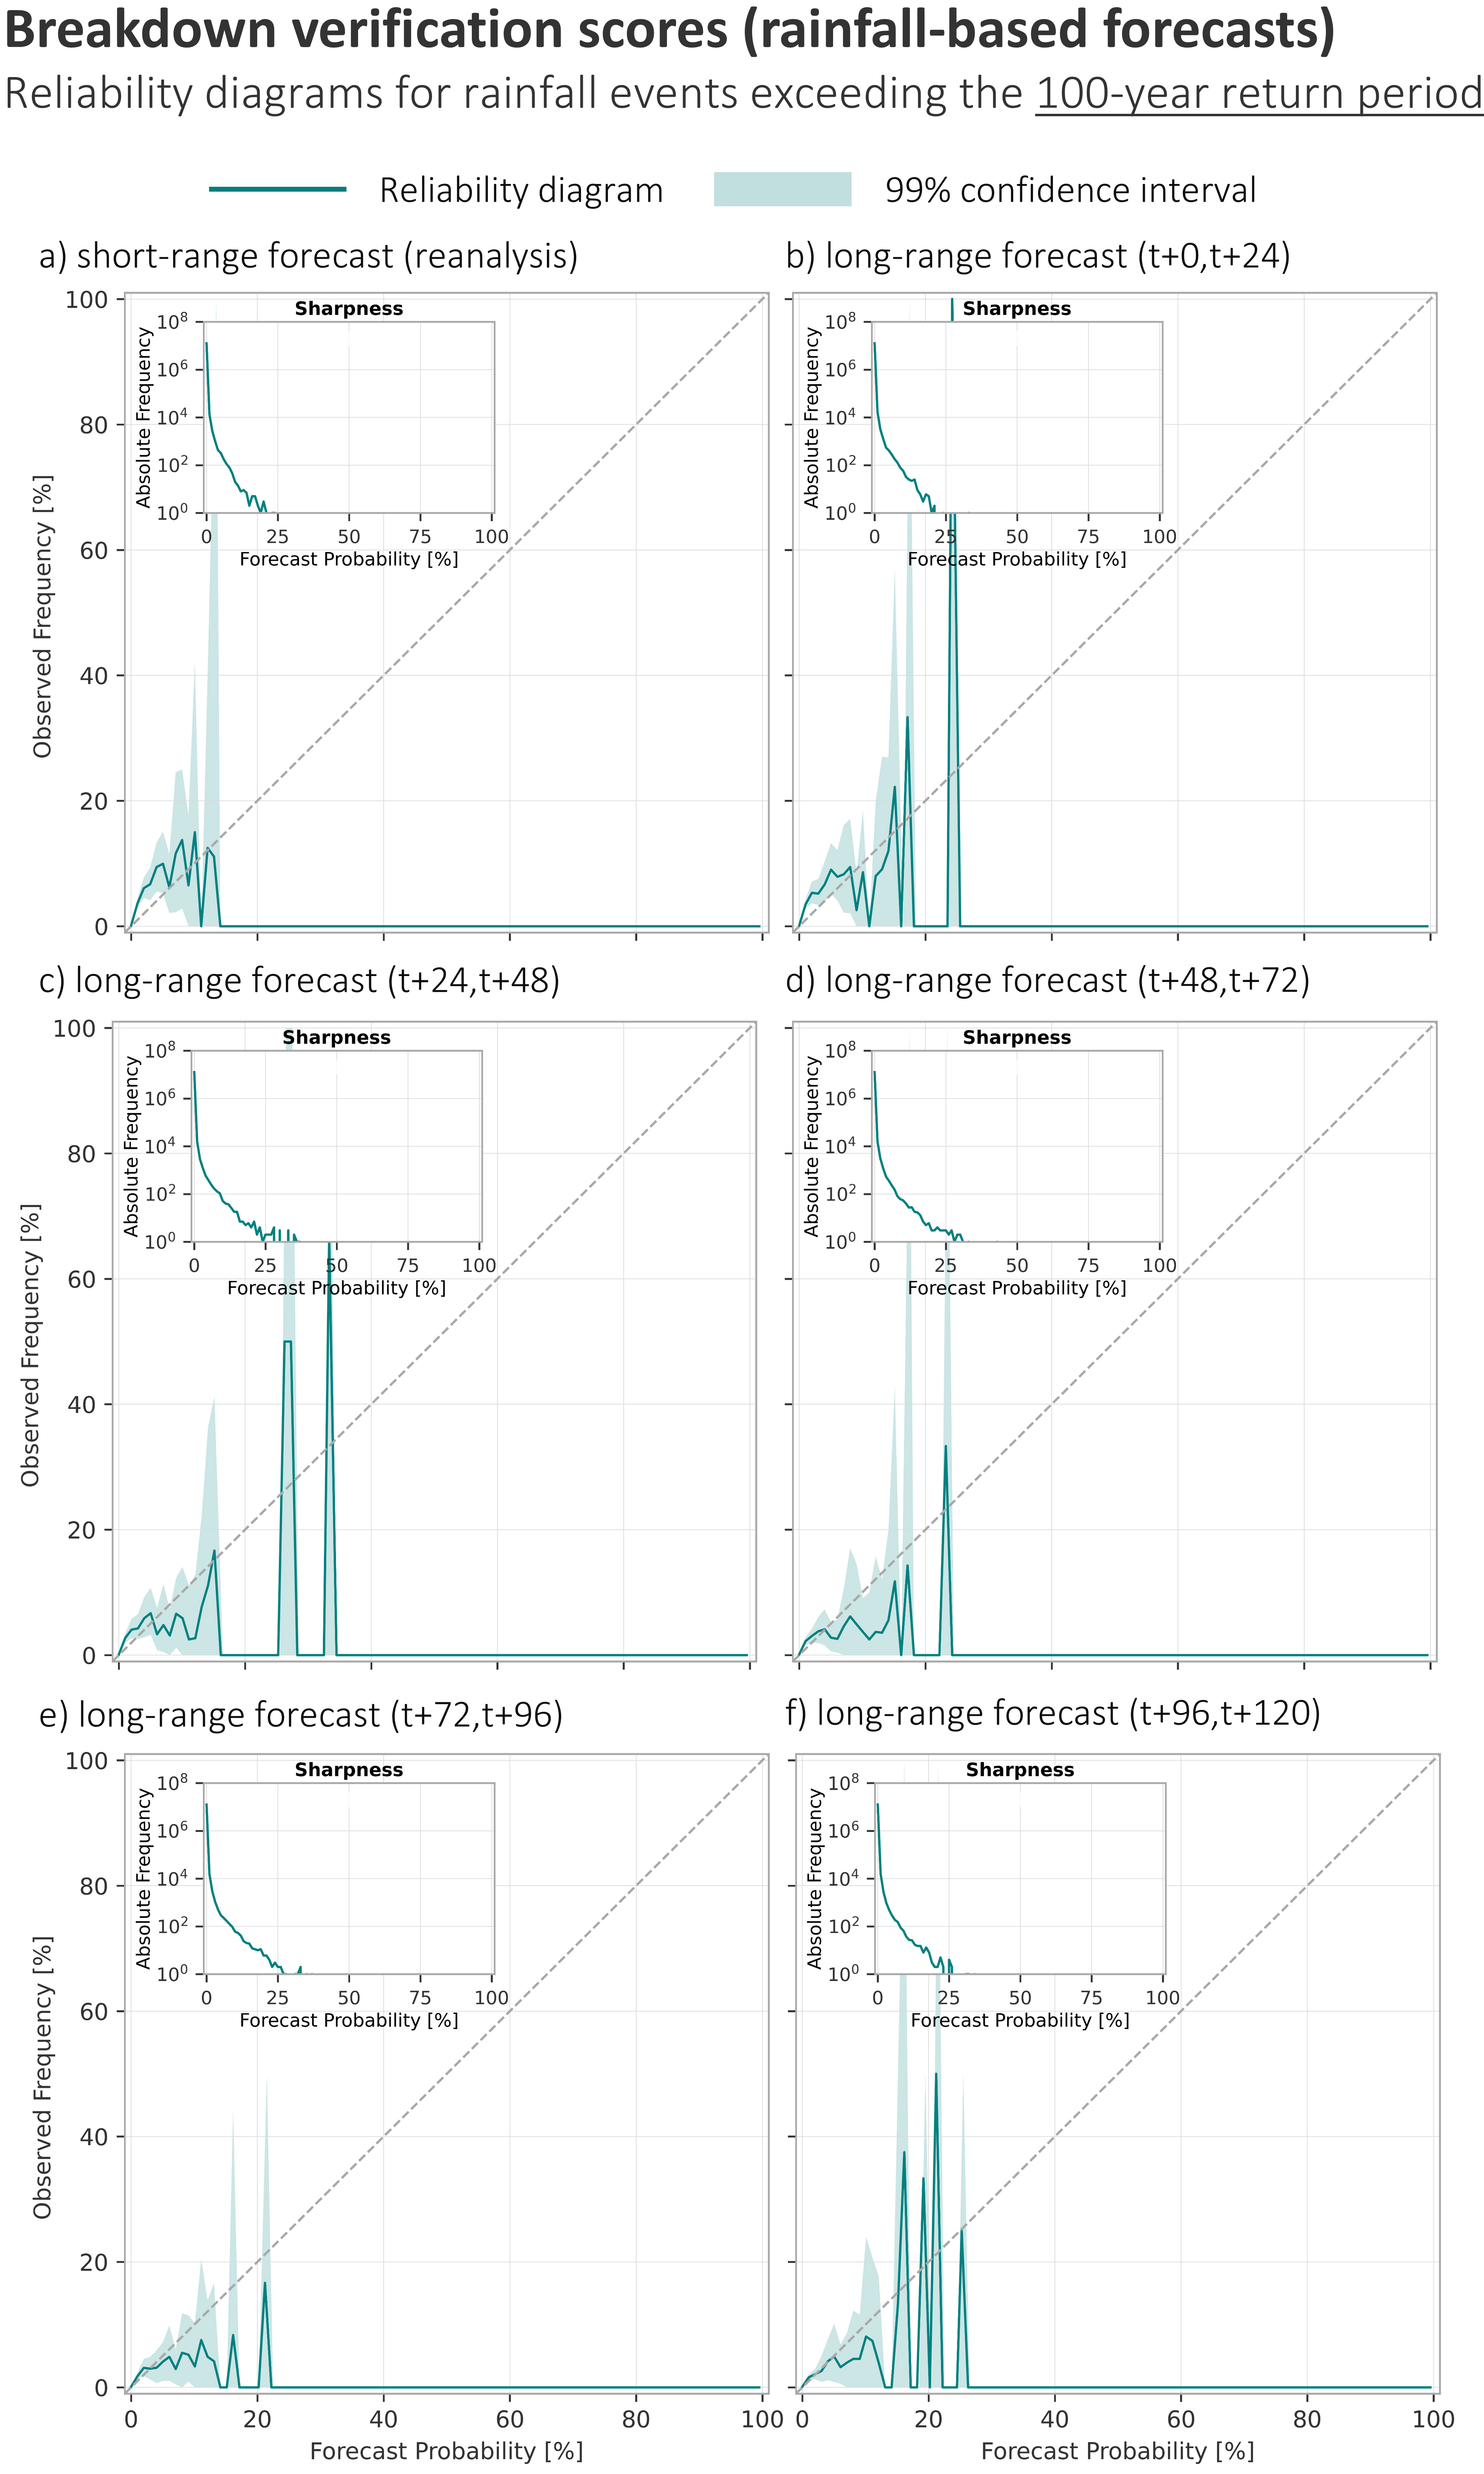
\includegraphics[width=\textwidth]{rainfall_based_ff_verif_breakdown_scores_rel_diag_100rp.png}
\caption{\textbf{Reliability diagrams for tp >= 5-year return period for the rainfall-based forecasts of areas at risk of flash floods built with ERA5-ecPoint.} Similar to Figure \ref{fig:rainfall_based_ff_verif_breakdown_scores_rel_diag_1rp}.}
\label{fig:rainfall_based_ff_verif_breakdown_scores_rel_diag_100rp}
\end{figure}


%%%%%%%%%%%%%%%%%%%%%
\section{Case Study: Storm Irma}
\label{flash_flood_focused_verification_rainfall_based_ff_CASE_STUDY}


%%%%%%%%%%%%%%%%%%%%%
\section{Discussions}
\label{flash_flood_focused_verification_rainfall_based_ff_DISCUSSIONS}


%%%%%%%%%%%%%%%%%%%%%
\section{Conclusions}
\label{flash_flood_focused_verification_rainfall_based_ff_CONCLUSIONS}
